\documentclass[11pt,a4paper]{article}

\def\nyear {2025}
\def\nterm {Winter}
\def\nlecturer {Ariel Rapaport}
\def\ncourse {Complex Analysis}

\makeatletter

% packages
\usepackage{amssymb,amsfonts,amsmath,calc,tikz,pgfplots,geometry,mathtools}
\usepackage{color}   % May be necessary if you want to color links
\usepackage[svgnames]{xcolor}
\usepackage[hidelinks]{hyperref}
\usepackage{forest}
\usepackage{commath} % ew
\usepackage{esvect} % \vv makes vectors
\usepackage{centernot} % for the comparison
\usepackage{esdiff}
\usepackage{esint}
\usepackage{amsthm}
\usepackage{fancyhdr}
\usepackage{bm}
\usepackage{witharrows}
\usepackage{bookmark}
\usepackage{tikz-cd}
\usepackage{quiver}
\usepackage{bbm}
\usepackage{textcomp}
\usepackage{float}
\usepackage{gensymb}
\usepackage{cleveref}
\usepackage{environ}
\usepackage{comment}
\usepackage{cancel}
\usepackage{xparse}

% Inevitable cs
\usepackage{listings}
\usepackage[]{algorithm2e}

% tikz libraries
\usetikzlibrary{positioning}
\usetikzlibrary{matrix}
\usetikzlibrary{arrows}
\usetikzlibrary{bending}
\usetikzlibrary{arrows.meta}
\usetikzlibrary{decorations.markings}
\usetikzlibrary{decorations.pathreplacing}
\usetikzlibrary{decorations.markings}
\usetikzlibrary{patterns}
\usetikzlibrary{backgrounds}

% Page style setup
\pagestyle{fancy}
\fancyhfoffset{0pt}
\renewcommand{\headwidth}{\textwidth}
\geometry{margin=1in}
\pgfplotsset{compat=1.18}
\setlength{\headheight}{14.6pt}
\addtolength{\topmargin}{-1.6pt}
\hypersetup{
    colorlinks=false,
    linktoc=section,
    linkcolor=black,
}

%% maketitle setup
\ifx \nauthor\undefined
  \def\nauthor{Yeheli Fomberg}
\else
\fi

\ifx \nemail\undefined
  \def\nemail{\href{mailto:yp@campus.technion.ac.il}
  {\texttt{<yp@campus.technion.ac.il>}}}
\else
\fi

\ifx \ncoursehead \undefined
  \def\ncoursehead{\ncourse}
\fi

\lhead{\emph{\nouppercase{\leftmark}}}
\ifx \nextra \undefined
  \rhead{
    \ifnum\thepage=1
    \else
      \ncoursehead
    \fi}
\else
  \rhead{
    \ifnum\thepage=1
    \else
      \ncoursehead \ (\nextra)
    \fi}
\fi

\def\notes{notes}
\def\problems{problems}

\ifx \ntype \undefined
  \def\ntype{notes}
\else
\fi

\ifx \ntype \notes
  \let\@real@maketitle\maketitle
  \renewcommand{\maketitle}{\@real@maketitle\begin{center}
  \begin{minipage}[c]{0.9\textwidth}\centering\footnotesize
  These notes are not endorsed by the lecturers.
  I have revised them outside lectures to incorporate supplementary
  explanations, clarifications, and material for fun.
  While I have strived for accuracy, any errors or misinterpretations 
  are most likely mine.
  \end{minipage}\end{center}}
\else
  \ifx \ntype \problems
    \let\@real@maketitle\maketitle
    \renewcommand{\maketitle}{\@real@maketitle\begin{center}
    \begin{minipage}[c]{0.9\textwidth}\centering\footnotesize
    These problems are mostly based on the problem sets I was given
    when taking the course.
    
    While I have strived for accuracy and completeness,
    some of the problems would not have been here without the help of
    friends.
    \end{minipage}\end{center}}
  \else
  \fi
\fi


% theorem environments
\theoremstyle{definition}
\newtheorem{definition}{Definition}[section]
\newtheorem{remark}{Remark}[section]
\newtheorem{example}{Example}[section]
\newtheorem{exercise}{Exercise}[section]
\newtheorem{paradox}{Paradox}[section]
\newtheorem{entry}{Entry}[section]
\newtheorem*{solution}{Solution}
\newtheorem*{question}{Question}
\newtheorem*{answer}{Answer}
\newtheorem*{problem}{Problem}
\theoremstyle{plain}
\newtheorem{theorem}{Theorem}[section]
\newtheorem{proposition}[theorem]{Proposition}
\newtheorem{lemma}[theorem]{Lemma}
\newtheorem{corollary}[theorem]{Corollary}
\newenvironment{proofof}[1]{%
    \renewcommand{\proofname}{Proof of #1}%
    \begin{proof}
}{%
    \end{proof}
}
% tikz customization
\pgfarrowsdeclarecombine{twolatex'}{twolatex'}{latex'}{latex'}{latex'}{latex'}
\tikzset{->/.style = {decoration={markings,
                                  mark=at position 0.999
                                  with {\arrow[scale=2]{latex'}}},
                      postaction={decorate}}}
\tikzset{<-/.style = {decoration={markings,
                                  mark=at position 0.001 with {\arrowreversed[scale=2]{latex'}}},
                      postaction={decorate}}}
\tikzset{-->/.style = {decoration={markings,
                                  mark=at position 0.999
                                  with {\arrow[scale=2]{latex'[sep=0pt -2.5]}}},
                      postaction={decorate}}}
\tikzset{<--/.style = {decoration={markings,
                                  mark=at position 0.001
                                  with {\arrowreversed[scale=2]{latex'[sep=0pt -2.5]}}},
                      postaction={decorate}}}
\tikzset{<->/.style = {decoration={markings,
                                  mark=at position 0.001 with {\arrowreversed[scale=2]{latex'}},
                                  mark=at position 0.999 with {\arrow[scale=2]{latex'}},},
                      postaction={decorate}}}
\tikzset{->-/.style = {decoration={markings,
    mark=at position 0.50+0.225/#1 with {\arrow[scale=2]{latex'}}},
                      postaction={decorate}}}
\tikzset{-<-/.style = {decoration={markings,
                                   mark=at position 0.50-0.225/#1 with {\arrowreversed[scale=2]{latex'}}},
                       postaction={decorate}}}
\tikzset{->>/.style = {decoration={markings,
                                  mark=at position 1 with {\arrow[scale=2]{latex'}}},
                      postaction={decorate}}}
\tikzset{<<-/.style = {decoration={markings,
                                  mark=at position 0 with {\arrowreversed[scale=2]{twolatex'}}},
                      postaction={decorate}}}
\tikzset{<<->>/.style = {decoration={markings,
                                   mark=at position 0 with {\arrowreversed[scale=2]{twolatex'}},
                                   mark=at position 1 with {\arrow[scale=2]{twolatex'}}},
                       postaction={decorate}}}
\tikzset{->>-/.style = {decoration={markings,
                                   mark=at position 0.50+0.450/#1 with {\arrow[scale=2]{twolatex'}}},
                       postaction={decorate}}}
\tikzset{-<<-/.style = {decoration={markings,
                                   mark=at position 0.50-0.450/#1 with {\arrowreversed[scale=2]{twolatex'}}},
                       postaction={decorate}}}

\pgfarrowsdeclare{biggertip}{biggertip}{%
  \setlength{\arrowsize}{1pt}
  \addtolength{\arrowsize}{.1\pgflinewidth}
  \pgfarrowsrightextend{0}
  \pgfarrowsleftextend{-5\arrowsize}
}{%
  \setlength{\arrowsize}{1pt}
  \addtolength{\arrowsize}{.1\pgflinewidth}
  \pgfpathmoveto{\pgfpoint{-5\arrowsize}{4\arrowsize}}
  \pgfpathlineto{\pgfpointorigin}
  \pgfpathlineto{\pgfpoint{-5\arrowsize}{-4\arrowsize}}
  \pgfusepathqstroke
}
\tikzset{
	EdgeStyle/.style = {>=biggertip}
}

\tikzset{circ/.style = {fill, circle, inner sep = 0, minimum size = 3}}
\tikzset{scirc/.style = {fill, circle, inner sep = 0, minimum size = 1.5}}
\tikzset{mstate/.style={circle, draw, black, text=black, minimum width=0.7cm}}

\tikzset{eqpic/.style={baseline={([yshift=-.5ex]current bounding box.center)}}}

\definecolor{mblue}{rgb}{0.2, 0.3, 0.8}
\definecolor{morange}{rgb}{1, 0.5, 0}
\definecolor{mgreen}{rgb}{0, 0.4, 0.2}
\definecolor{mred}{rgb}{0.5, 0, 0}

% topology
\DeclareMathOperator{\dfr}{dfr} % deformation retract
\newcommand{\Cells}{\text{Cells}}
\newcommand{\RP}{\mathbb{RP}}
\newcommand{\CP}{\mathbb{CP}}

% order theory
\newcommand{\join}{\vee}
\newcommand{\meet}{\wedge}

% algebraic geometry
\DeclareMathOperator{\Rad}{Rad} % Radical of modules
\DeclareMathOperator{\Spec}{Spec}
% \renewcommand{\div}{\mathrm{div}} % divisors
\DeclareMathOperator{\Mer}{Mer} % Meromorphic functions
\DeclareMathOperator{\Exc}{Exc} % Exceptional divisor
\DeclareMathOperator{\Td}{Td} % Todd classes

% algebra

\DeclareMathOperator{\trdeg}{tr.deg.}
\DeclareMathOperator{\odd}{odd}
\DeclareMathOperator{\even}{even}
\DeclareMathOperator{\lcm}{lcm}
\DeclareMathOperator{\ord}{ord}
\DeclareMathOperator{\codim}{codim}
\DeclareMathOperator{\Ann}{Ann}
\DeclareMathOperator{\Ext}{Ext}
\DeclareMathOperator{\Sym}{Sym}
\DeclareMathOperator{\Out}{Out}
\DeclareMathOperator{\Aut}{Aut}
\DeclareMathOperator{\End}{End}
\DeclareMathOperator{\Inn}{Inn}
\DeclareMathOperator{\Mat}{Mat}
\DeclareMathOperator{\Fix}{Fix}
\DeclareMathOperator{\std}{std}
\DeclareMathOperator{\sgn}{sgn}
\DeclareMathOperator{\adj}{adj}
\DeclareMathOperator{\id}{id}
\DeclareMathOperator{\op}{op}
\DeclareMathOperator{\tr}{tr}
\DeclareMathOperator{\diag}{diag}
\DeclareMathOperator{\rank}{rank}
\DeclareMathOperator{\rk}{rk}
\DeclareMathOperator{\coker}{coker}
\DeclareMathOperator{\Mult}{Mult} % multiplier algebra
\DeclareMathOperator{\Frac}{Frac} % fraction field
\DeclareMathOperator{\Rat}{Rat}
\DeclareMathOperator{\Gal}{Gal}
\newcommand{\ioplus}{\overset{\text{int}}{\oplus}} % interior direct sum
\newcommand{\GG}{\mathcal G} % Galois correspondence
\newcommand{\FF}{\mathcal F} % Galois correspondence
\newcommand{\cupp}{\smile} % cup product
\newcommand{\capp}{\frown} % cap product
\newcommand{\actson}{\curvearrowright}
\newcommand{\bra}{\left\langle}
\newcommand{\ket}{\right\rangle}
\newcommand{\idealin}{\triangleleft\,}
\newcommand{\normalin}{\triangleleft\,}
\newcommand{\ip}[2]{\left\langle #1, #2 \right\rangle}
\newcommand{\bigslant}[2]
{{\raisebox{.2em}{$#1$}\left/\raisebox{-.2em}{$#2$}\right.}}
\newcommand{\properideal}{%
  \mathrel{\ooalign{$\lneq$\cr\raise.22ex\hbox{$\lhd$}\cr}}}

% categories
\newcommand{\cat}[1]{\mathbf{#1}}
\newcommand{\Ch}{\cat{Ch}} % Chain complexes   
\newcommand{\Set}{\cat{Set}}
\newcommand{\Grp}{\cat{Grp}}
\newcommand{\Ab}{\cat{Ab}}
\newcommand{\Ring}{\cat{Ring}}
\newcommand{\CRing}{\cat{CRing}}
\newcommand{\Top}{\cat{Top}}
\newcommand{\Vect}{\cat{Vect}}
\newcommand{\cmod}{\cat{mod}}

%% matrix groups
\newcommand{\GL}{\mathrm{GL}}
\newcommand{\Or}{\mathrm{O}}
\newcommand{\PGL}{\mathrm{PGL}}
\newcommand{\PSL}{\mathrm{PSL}}
\newcommand{\PSO}{\mathrm{PSO}}
\newcommand{\PSU}{\mathrm{PSU}}
\newcommand{\SL}{\mathrm{SL}}
\newcommand{\msl}{\mathrm{sl}}
\newcommand{\SO}{\mathrm{SO}}
\newcommand{\Spin}{\mathrm{Spin}}
\newcommand{\Sp}{\mathrm{Sp}}
\newcommand{\SU}{\mathrm{SU}}
\newcommand{\U}{\mathrm{U}}
\let\char\relax
\newcommand{\char}{\text{char}}

% analysis
\renewcommand{\Re}{\mathrm{Re}}
\renewcommand{\Im}{\mathrm{Im}}
\NewDocumentCommand{\dx}{o}{
  \IfNoValueTF{#1}
    {\dif x}                  % if no optional argument
    {\dif^{#1} \!x}         % if optional argument
}
\NewDocumentCommand{\dy}{o}{
  \IfNoValueTF{#1}
    {\dif y}                  % if no optional argument
    {\dif^{#1} \!y}         % if optional argument
}
\newcommand{\dt}{\dif t}
\newcommand{\du}{\dif u}
\newcommand{\dv}{\dif v}
\newcommand{\dz}{\dif z}
\newcommand{\ds}{\dif s}
\newcommand{\dw}{\dif w}
\newcommand{\dr}{\dif r}
\newcommand{\dm}{\dif m}
\newcommand{\df}{\dif f}
\newcommand{\dV}{\dif V}
\newcommand{\dS}{\dif S}
\newcommand{\dA}{\dif \mathrm{A}}
\newcommand{\dmu}{\dif \mu}
\newcommand{\dnu}{\dif \nu}
\newcommand{\dtheta}{\dif \theta}
\newcommand{\domega}{\dif \omega}
\newcommand{\dsigma}{\dif \sigma}
\newcommand{\dtau}{\dif \tau}
\newcommand{\dvarphi}{\dif \varphi}
\renewcommand{\dif}{\mathrm{d}}
\renewcommand{\Dif}{\mathrm{D}}
\renewcommand{\triangle}{\Delta}
\newcommand{\ptriangle}{\partial \triangle}
\DeclareMathOperator{\im}{im}
\DeclareMathOperator{\cis}{cis}
\DeclareMathOperator{\rot}{rot}
\DeclareMathOperator{\vspan}{span}
\DeclareMathOperator{\grad}{grad}
\DeclareMathOperator{\curl}{curl}
\DeclareMathOperator{\esssup}{esssup}
\newcommand{\hodge}{{\mathnormal{\star}}}
\DeclareMathOperator{\range}{range}
\DeclareMathOperator{\Hom}{Hom}
\DeclareMathOperator{\Int}{Int}
\DeclareMathOperator{\Conv}{Conv} % convex hull
\newcommand{\ind}{\mathbbm{1}}
\DeclareMathOperator{\Res}{Res}
\DeclareMathOperator{\graph}{graph}
\DeclareMathOperator{\diam}{diam}
\DeclareMathOperator{\supp}{supp}
\DeclareMathOperator{\Vol}{Vol} % Volume
\DeclareMathOperator{\Area}{Area} % Area
\DeclareMathOperator{\area}{area}
\DeclareMathOperator{\Ind}{Ind} % Index
\newcommand{\length}{\mathrm{length}}

% logic
\DeclareMathOperator{\MOD}{MOD}
\DeclareMathOperator{\Theory}{Theory}
\newcommand{\notimplies}{%
  \mathrel{{\ooalign{\hidewidth$\not\phantom{=}$\hidewidth\cr$\implies$}}}}

% nice
\newcommand{\half}{\frac{1}{2}}
\newcommand{\pair}{\del}
\newcommand{\taking}[1]{\xrightarrow{#1}}
\newcommand{\otaking}[1]{\xleftarrow{#1}}
\newcommand{\inv}{^{-1}}
\newcommand{\ot}{\leftarrow}
\newcommand{\ninfty}{-\infty}
\newcommand{\pinfty}{+\infty}
\newcommand{\floor}[1]{\left\lfloor #1 \right\rfloor}
\newcommand{\ceil}[1]{\left\lceil #1 \right\rceil}
\newcommand{\viff}{\Big\Updownarrow} % vertical iff
\newcommand{\bmid}{\,\middle\vert\,} % big mid

% probability
\newcommand{\Prob}{\mathbf{P}}
\renewcommand{\vec}[1]{\boldsymbol{\mathbf{#1}}}
\DeclareMathOperator{\Bin}{Bin}
\DeclareMathOperator{\Geo}{Geo}
\DeclareMathOperator{\Poi}{Poi}
\DeclareMathOperator{\Exp}{Exp}
\DeclareMathOperator{\Var}{Var} % Variance
\DeclareMathOperator{\Cov}{Cov}

% special letters
\newcommand{\N}{\mathbb{N}}
\newcommand{\Z}{\mathbb{Z}}
\newcommand{\Q}{\mathbb{Q}}
\newcommand{\R}{\mathbb{R}}
\newcommand{\C}{\mathbb{C}}
\newcommand{\F}{\mathbb{F}}
\newcommand{\E}{\mathbf{E}}
\newcommand{\D}{\mathbb{D}}
\renewcommand{\H}{\mathbb{H}}
\newcommand{\ps}{\mathcal{P}}
\newcommand{\M}{\mathcal{M}}
\renewcommand{\L}{\mathcal{L}}
\renewcommand{\O}{\mathcal{O}}
\renewcommand{\U}{\mathcal{U}}
\newcommand{\Omicron}{O}
\newcommand{\powerset}{\mathcal{P}}

% text
\newcommand{\st}{\text{ s.t. }}
\newcommand{\tand}{\quad \text{and} \quad}
\newcommand{\tor}{\quad \text{or} \quad}
\newcommand{\stand}{\text{ and }}
\newcommand{\stor}{\text{ or }}
\renewcommand{\tt}[1]{\textnormal{\textbf{(#1).}}} %tt=theorem title GET RID OF

% title format
\title{\textbf{\ncourse}}

\ifx \ntype \notes
  \author{Notes taken by \nauthor\, \nemail \\ Based on lectures by \nlecturer}
  \date{\nterm\ \nyear}
\else
  \ifx \ntype \problems
    \author{These problems were solved by \nauthor \\ \nemail}
  \else
  \fi
\fi

\makeatother


% \excludecomment{exercise}
% \excludecomment{proposition}
% \excludecomment{remark}
% \excludecomment{proof}
% \excludecomment{theorem}
% \excludecomment{example}
% \excludecomment{corollary}
% \excludecomment{lemma}
%
% % \RenewEnviron{definition}{\begin{definition}\BODY\end{definition}}
% %
% % % Comment out normal text
% \renewcommand{\theenumi}{} % Hide numbering if used
% \renewcommand{\labelenumi}{} % Hide bullets if used
% \renewcommand{\paragraph}[1]{}

\begin{document}
\maketitle

% Insert cool image here

\newpage
\tableofcontents
\newpage

\section{Introduction}

\subsection{Complex numbers and the complex plane}

\subsubsection{Preliminaries}

\begin{definition}[Complex number]
  A complex number is an expression of the form $x + yi$ such that
  $x,y \in \R$ and $i$ is a `imaginary number' not in $\R$.
  We denote
  \[
      \Re(z) := x \tand \Im(z) := y.
  \]
  If $\Im(z) = 0$ then $z$ is said to be a real number, and if
  $\Re(z) = 0$ then it is said to be purely imaginary.
\end{definition}
\begin{remark}
The set of all complex numbers is denoted as $\C$ and it can be made into
a field with the following operations.
\[
  z_1 + z_2 = (x_1 + x_2) + (y_1 + y_2) i \tand
  z_1 z_2 = (x_1 x_2 - y_1 y_2) + (x_1 y_2 + y_1 x_2) i.
\]
The field $\C$ is called the complex plane.

Note that $i^2 = -1$.
Also note that $T(x + y i) = (x, y)$ is a bijection between $\C$ and $\R$ and
moreover, we have that $T$ is additive.
That is
\[
  T(z_1 + z_2) = T(z_1) + T(z_2)
\]
which gives complex addition a geometric meaning.

\begin{center}
  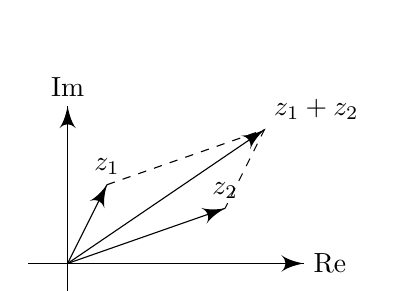
\begin{tikzpicture}
    \draw [->] (-0.5, 0) -- (3, 0) node [right] {Re};
    \draw [->] (0, -0.5) -- (0, 2) node [above] {Im};
    \draw [->] (0, 0) -- (.5, 1) node [above] {$z_1$};
    \draw [->] (0, 0) -- (2, .7) node [above] {$z_2$};
    \draw [->] (0, 0) -- (2.5, 1.7) node [anchor=south west] {$z_1 + z_2$};
    \draw [dashed] (.5, 1) -- (2.5, 1.7) -- (2, .7);
  \end{tikzpicture}
\end{center}

The absolute value of a complex number $x + y i = z \in \C$ is defined by
\[
  |z| = \sqrt{x^2 + y^2}.
\]
Note that $|z| = \norm{(x,y)}= \norm{T(z)}$ where $\norm{\cdot}$ is the standard
Euclidean norm on $\R^2$.

This implies that $|z - w|$ should be considered the distance between natural
numbers $z$, $w$.
Because we have that $|z| = \norm{T(z)}$ we also have that the triangle
inequality holds:
\[
  |z + w| \le |z| + |w| \text{ for all } z,w \in \C.
\]
\end{remark}
\begin{definition}[Complex conjugate]
  The complex conjugate of $x + y i = z \in C$ is the complex number
  $x - y i$. The complex conjugate of $z$ is denoted $\bar{z}$.
\end{definition}

\begin{center}
  \begin{tikzpicture}
    \draw [->] (-0.5, 0) -- (3, 0) node [right] {Re};
    \draw [->] (0, -1) -- (0, 2) node [above] {Im};
    \draw [->] (0, 0) -- (2, .7) node [above] {$z_2$};
    \draw [->] (0, 0) -- (2, -.7) node [above] {$\bar z_2$};
  \end{tikzpicture}
\end{center}

\begin{remark}
It is easy to verify that
\[
  \Re(z) = \frac{z + \bar{z}}{2} \tand 
  \Re(z) = \frac{z - \bar{z}}{2 i} \tand
  |z|^2 = z \bar{z}.
\]

Given $\theta$ we can denote $e^{i \theta} = \cos \theta + i \sin \theta$,
and then describe any complex number $z \in \C$ as $r e^{i \theta}$
for some $\theta \in [0, 2\pi)$ and $r > 0$.
We get that $|z| = |r e^{i \theta}| = r$.
We also have that $\theta$ describes the angle of $z$ with the $x$-axis
and it is usually denoted $\theta = \arg(z)$.
\end{remark}

\subsubsection{Convergence}

\begin{definition}[Convergence]
  We say that the sequence $\set{z_n}_{n \geq 1} \subset \C$ converges
  to some $z_0 \in \C$ if $|z - z_0| \taking{n \to \infty} 0$.
  In this case, we call $z_0$ the limit of the sequence of
  $\set{z_n}_{n \geq 1}$.
\end{definition}

\begin{remark}
  It is easy to verify that the limit is unique, and that
  $z_n \taking{n \to \infty} z$ if and only if
  $T(z_n) \taking{n \to \infty} T(z)$ in the Euclidean metric.
\end{remark}

\begin{definition}[Cauchy sequence]
  A sequence $\set{z_n}_{n \geq 1}$ is said to be a Cauchy sequence if for
  all $\epsilon > 0$ there exists $N > 1$ such that for all $n,m > N$
  we have that $|z_n - z_m| < \epsilon$.
\end{definition}

\begin{proposition}
  The complex plane $\C$ is complete.
  That is, every Cauchy sequence converges in $\C$.
\end{proposition}
\begin{proof}
  The proof follows immediately from the known fact that $\R$ is complete
  and the previous remark.
\end{proof}

\subsubsection{Sets in the complex plane}

\begin{definition}[Open disc]
  For $z_0 \in \C$ and $r > 0$ we set
  \[
      D_r(z_0) := \set{z \in \C \colon |z - z_0| < r}.
  \]
  We call $D_r(z_0)$ the open disc at center $z_0$ with radius $r$.
\end{definition}


\begin{definition}[Closed disc]
  For $z_0 \in \C$ and $r > 0$ we set
  \[
      \overline D_r(z_0) := \set{z \in \C \colon |z - z_0| \le r}.
  \]
  We call $\overline D_r(z_0)$ the closed disc at center $z_0$ with
  radius $r$.
\end{definition}

\begin{definition}[Circle]
  For $z_0 \in \C$ and $r > 0$ we set
  \[
      C_r(z_0) := \set{z \in \C \colon |z - z_0| = r}.
  \]
  We call $C_r(z_0)$ the circle at center $z_0$ with radius $r$.
\end{definition}

\begin{definition}[Interior point]
  Given $\Omega \subset \C$, we say that $z \in \Omega$ is an interior
  point of $\Omega$ if exists $r > 0$ such that $D_r(z) \subset \Omega$.
\end{definition}

\begin{definition}[Interior of a set]
  Given $\Omega \subset \C$, we say that the interior of $\Omega$ is
  the collection of all interior points of $\Omega$.
  We denote the interior of $\Omega$ by $\Int(\Omega)$.
\end{definition}

\begin{definition}[Open set]
  Given $\Omega \subset \C$, we say that $\Omega$ is an open set if
  $\Int(\Omega) = \Omega$.
\end{definition}

\begin{definition}[Closed set]
  Given $\Omega \subset \C$, we say that $\Omega$ a closed set if
  $\Omega^c := \C \setminus \Omega$ is open.
\end{definition}

\begin{definition}[Limit point]
  Given $\Omega \subset \C$, we say that $z \in \Omega$ is a limit
  point of $\Omega$ if there exists a sequence
  $\set{z_n}_{n=1}^{\infty} \subset \Omega$ such that
  $z_n \neq z$ for all $n \geq 1$ and $z_n \taking{n \to \infty} z$.
\end{definition}

\begin{proposition}
  Let $\Omega \subset \C$ be given.
  Then $\Omega$ is closed if and only if it contains
  all of its limit points.
\end{proposition}
\begin{proof}
  Suppose that $\Omega$ is not closed.
  Then $\C \setminus \Omega$ is not open,
  which implies that there exists $z \in \C \setminus \Omega$ such
  that for all $n \geq 1$ there exists $z_n \in \Omega \cap D_{1/n}(z)$.
  Since it is clear that $z \neq z_n \taking{n \to \infty} z$,
  we get that $z$ is a limit point of $\Omega$ which is not contained
  in $\Omega$.
  This completes one direction of the proposition.

  Next suppose that there exists $z \in \C \setminus \Omega$ which is
  a limit point of $\Omega$.
  Thus it can't be an interior point of $\C \setminus \Omega$,
  which means that $\C \setminus \Omega$ is not open,
  so $\Omega$ is not closed which completes the proof.
\end{proof}

\begin{definition}[Closure]
  Let $\Omega \subset \C$ be given.
  The closure of $\Omega$, denoted $\overline \Omega$, is defined
  as
  \[
      \overline \Omega =
      \Omega \cup
      \set{z \in \C \mid \text{$x$ is a limit point of $\Omega$}}.
  \]
\end{definition}

\begin{remark}
  Note that $\Omega$ is closed if and only if $\overline \Omega = \Omega$.
\end{remark}

\begin{definition}[Boundary]
  The boundary of $\Omega \subset \C$ is denoted by $\partial \Omega$
  and defined by $\partial \Omega := \Omega \setminus \Int(\Omega)$.
\end{definition}

\begin{definition}[Diameter]
  Given $\Omega \subset \C$, we define the diameter of $\Omega$ as
  \[
      \diam(\Omega) := \sup\set{|z - w| \colon z,w \in \Omega}.
  \]
\end{definition}

\begin{definition}[Bounded set]
  Given $\Omega \subset \C$, we say that $\Omega$ is bounded if
  $\diam(\Omega) < \infty$.
\end{definition}

\begin{remark}
  It is clear that a set $\Omega \subset \C$ is bounded if and only if
  there exists $z_0 \in \C$ and $r > 0$ such that $\Omega \subset D_r(z_0)$.
\end{remark}

\begin{definition}[Compact set]
  A subset $\Omega$ of $\C$ is said to be compact if it is closed and 
  bounded.
\end{definition}

\begin{theorem}[Bolzano--Weierstrass theorem]
  A subset $\Omega$ in $\C$ is compact if and only if every seqeuence
  $\set{z_n}_{n \geq 1}$ has a subsequence $\set{z_{n_k}}$ such that
  $z_{n_k} \taking{k \to \infty} z$ for some $z \in \C$.
\end{theorem}
\begin{remark}
  Another formulation of the Bolzano--Weierstrass theorem is that a subset
  of $\R^n$ (equivalently of $\C$) is sequencially compact if and only if
  it is closed and bounded.
  This is why it is also occasionally called
  the sequential compactness theorem.
\end{remark}

\begin{theorem}[Cantor's intersection lemma]
  Let $\Omega_1, \Omega_2, \dots$ be nonempty compact subsets of $\C$.
  Suppose that $\Omega_{n+1} \subset \Omega_n$ for all $n \geq 1$,
  and that $\diam(\Omega_n) \taking{n \to \infty} 0$.
  Then $\cap_{n \geq 1} \Omega_n = \set{z}$ for some $z \in \C$.
\end{theorem}
\begin{proof}
  Choose $z_n \in \Omega_n$ for all $n \geq 1$.
  Because $\diam(\Omega) \taking{n \to \infty} 0$ we have that
  $\set{z_n}_{n \geq 1}$ is a Cauchy sequence and therefore it converges
  to some $z \in \C$. Because $\Omega_n$ is compact for every $n \geq 1$
  we get that $z \in \cap_{n \geq 1} \Omega_n$.
  This means that $\cap_{n \geq 1} \Omega_n \neq \emptyset$.

  Let $z,w \in \Omega$.
  Because $\diam \Omega \taking{n \to \infty} 0$ we have that
  $|z - w| \le 0$ and thus $z = w$ which implies that
  $\cap_{n \geq 1} \Omega_n = \set{z}$ which completes the proof.
\end{proof}

\begin{definition}[Connected open set]
  A nonempty open set $\Omega \subset \C$ is said to be connected if it does
  not contain disjoint nonempty open subsets $\Omega_1$, $\Omega_2$ such
  that $\Omega = \Omega_1 \cup \Omega_2$.
\end{definition}

\begin{definition}[Region]
  A connected open set in $\C$ is called a region.
\end{definition}

\begin{definition}[Connected closed set]
  A nonempty open set $\Omega \subset \C$ is said to be connected if it does
  not contain disjoint nonempty closed subsets $\Omega_1$, $\Omega_2$ such
  that $\Omega = \Omega_1 \cup \Omega_2$.
\end{definition}

\begin{remark}
  It can be shown that $\Omega$ is connected if and only if for any
  $z, w \in \Omega$ there exists a curve $\gamma \colon [0,1] \to \Omega$
  such that $\gamma(0) = z$ and $\gamma(1)$.
  This implies that open and closed discs, as well as circles, are
  connected.
\end{remark}

\subsubsection{Continuous functions}

\begin{definition}[Continuous function]
  Let $\Omega$ be a nonempty subset of $\C$ and let 
  $f \colon \Omega \to \C$ be given.
  We say that $f$ is continuous at a point $z_0 \in \Omega$ 
  if for all $\epsilon > 0$ there exists $\delta > 0$ so
  that $|f(z) - f(z_0)| < \epsilon$ for all $z \in \Omega$ with 
  $|z - z_0| < \delta$.
  We say that $f$ is continuous on $\Omega$ if it is continuous at every 
  $z_0 \in \Omega$.
\end{definition}

\begin{remark}
  It is easy to verify that the functions $\Im$, $\Re$, $|\cdot|$, and
  $\theta \mapsto e^{i \theta}$ are all continuous.
\end{remark}

\begin{proposition}
  The addition, product, and composition of continuous functions is continuous.
\end{proposition}

\begin{definition}[Bounded function]
  Let $\Omega$ be a nonempty subset of $\C$ and let 
  $f \colon \Omega \to \C$ be given.
  We say that $f$ is bounded if there exists $M > 0$ so that 
  $|f(z)| < M$ for all $z \in \Omega$.
  We say that $f$ attains a maximum if there exists $z_M \in \Omega$
  such that $f(z) \le f(z_M)$ for all $z \in \Omega$.
  We define when $f$ attains a minimum similarly.
\end{definition}

\begin{proposition}
  Let $\Omega$ be a nonempty compact subset of $\C$, and let 
  $f \colon \Omega \to \C$ be continuous.
  Then $f$ is bounded, and it attains its maximum and minimum on $\Omega$.
\end{proposition}

\subsection{Holomorphic functions}

\begin{definition}[Holomorphic function]
  \label{def:holomorphic-function}
  Let $\Omega$ be a nonempty open subset of $\C$ and let 
  $f \colon \Omega \to \C$ be given.
  We say that $f$ is holomorphic at a point $z \in \Omega$
  if the following limit exists
  \[
      f'(z) := \lim_{h \to 0} \frac{f(z + h) - f(z)}{h}.
  \]
  The number $f'(z)$ is called the derivative of $f$ at $z$.
  It is said that $f$ is holomorphic if it is holomorphic at every
  $z \in \Omega$.
  Given a closed subset $C \subset \Omega$, we say that $f$ is holomorphic
  on $C$ if there exists $C \subset \Omega' \subset \Omega$ so that
  $\Omega'$ is open and $f$ is holomorphic on $\Omega'$.
\end{definition}

\begin{remark}
  Note that $h$ is a complex number and can approach $0$ from any direction.
\end{remark}

\begin{remark}
  This is not a course in computations of complex derivatives.
  While it is important to know \Cref{def:holomorphic-function},
  there is no need to be able to visualize it like in analysis 1.
  Instead we use simple tricks and complex differentiation rules
  that can be seen in the problems section.
\end{remark}

\begin{remark}
  As we mentioned earlier, given a complex function in the form
  $f(x,y) = u(x) + i v(y)$ we can also represent it as a function
  by $f(z, \bar z)$ and thus it makes sense to define partial derivatives
  with respect to $z$ and $\bar z$.
  However, unlike partial derivatives with respect to $x$ or $y$,
  the most natural definition (the Wirtinger derivative) may seem a little
  pathological.
\end{remark}

\begin{definition}[Wirtinger derivative]
  We define the Wirtinger derivative as
  \begin{align*}
    &\diffp{f}{z} :=
    \half \diffp{f}{x} - \frac{i}{2} \diffp{f}{y} \\
    &\diffp{f}{{\bar z}} :=
    \half \diffp{f}{x} + \frac{i}{2} \diffp{f}{y}.
  \end{align*}
\end{definition}

\begin{definition}[Entire function]
  We say that $f \colon \C \to \C$ is entire if it is holomorphic on $\C$.
\end{definition}

\begin{remark}
  It is also useful to notice that $f \colon \Omega \to \C$ is holomorphic
  at $z \in \Omega$ if and only if there exist $a \in \C$, $r > 0$ with
  $D_r(z) \subset \Omega$, and a function $\psi \colon D_r(0) \to \C$ with
  $\lim_{h \to 0} \psi(h) = 0$, so that
  \[
    f(z + h) = f(z) + ah + h \psi(h) \text{ for all } h \in D_r(0).
  \]
  From this formulation is it clear that $f$ is continuous at $z$ whenever
  $f$ is holomorphic at $z$.
\end{remark}

\begin{example}
  It follows directly from the definition that the function $1/z$ is holomorphic
  on $\C \setminus \set{0}$ with $f'(z) = -1/z^2$. For all $0 \neq z \in \C$
  we have
  \[
    \lim_{h \to 0} \frac{f(z + h) - f(z)}{h} =
    \lim_{h \to 0} \frac{1}{h} \del{\frac{1}{z + h} - \frac{1}{z}} =
    \lim_{h \to 0} \frac{-1}{z (z + h)} =
    \frac{-1}{z^2}.
  \]
\end{example}

\begin{example}
  The function $f(z) = \bar z$ is not holomorphic. For any $z \in \C$ and
  $t \in \R$ we have that
  \[
    \frac{f(z + t) - f(z)}{t} = 1 \tand
    \frac{f(z + t i) - f(z)}{t i} = -1.
  \]
\end{example}

\begin{proposition}
  \label{prop:holo-is-linear}
  Let $\Omega \subset \C$ be open and let $f,g \colon \Omega \to \C$ be
  holomorphic at $z \in \Omega$. Then
  \begin{enumerate}
    \item[(1)] $f + g$ is holomorphic at $z$ with $(f + g)'(z) = f'(z) + g'(z)$.
    \item[(2)] $f g$ is holomorphic at $z$ with $(f g)'(z) = 
      f'(z)g(z) + f(z)g'(z)$.
  \end{enumerate}
\end{proposition}

\begin{proof}
  We will only prove $(2)$ because the proof of $(1)$ is much simpler.
  Because $f$ and $g$ are holomorphic at $z$, they are also continuous
  there. Thus,
  \begin{align*}
    \lim_{h \to 0} \frac{(f g)(z + h) - (f g)(z)}{h} &=
    \lim_{h \to 0} \del{\frac{f(z + h) - f(z)}{h} g(z + h) + 
  f(z) \frac{g(z + h) - g(z)}{h}} \\ &=
    f'(z)g(z) + f(z)g'(z),
  \end{align*}
  which completes the proof.
\end{proof}

\begin{corollary}
  It's quite easy to prove that constant function of the form $f(z) = c$
  for some $c \in \C$ and $f(z) = z$ are holomorphic.
  It follows immediately from \Cref{prop:holo-is-linear} that all polynomials,
  functions of the form $p(z) = \sum_{k=0}^{n} a_k z^k$ are entire, with
  $p'(z) = \sum_{k=1}^{n} k a_k z^{k-1}$ for all $z \in \C$.
\end{corollary}

\begin{proposition}
  A composition of holomorphic functions at $z$ is holomorphic at $z$, with
  $(g \circ f)'(z) = g'(f(z)) f'(z)$.
\end{proposition}

\begin{corollary}
  Let $\Omega \subset \C$ be open and let $f,g \colon \Omega \to \C$ be
  holomorphic at $z \in \Omega$.
  Suppose also that $g(z) \neq 0$.
  Then $f/g$ is holomorphic at $z$ with
  \[
    (f/g)'(z) = \frac{f'(z)g(z) + f(z)g'(z)}{g(z)^2}.
  \]
\end{corollary}
\begin{proof}
  Let $h \colon \C \setminus \set{0} \to \C$ be with $h(z) = 1/z$.
  We now have that
  \begin{align*}
    (f/g)'(z) &=
    (f \cdot (h \circ g))'(z) =
    f'(z)(h \circ g)(z) + f(z)(h \circ g)'(z) \\ &=
    f'(z)/g(z) + f(z)h'(g(z))g'(z) =
    f'(z)/g(z) - f(z)g(z)^{-2}g'(z).
  \end{align*}
\end{proof}

\begin{remark}
Recall that $T \colon \C \to \R^2$ is the operator $T(x + y i) = (x,y)$.
\end{remark}

\renewcommand*{\arraystretch}{1.25}
\begin{proposition}
  \label{prop:pd}
  Let $\Omega \subset \C$ be open, let $f \colon \Omega \to \C$, let 
  $u,v \colon T(\Omega) \to \R$ be with $f(x + y i) = u(x,y) + i v(x,y)$
  for $x + i y \in \Omega$, and let $F \colon T(\Omega) \to \R^2$ be with
  $F(x,y) = (u(x,y), v(x,y))$ for $(x,y) \in T(\Omega)$.
  Fix $x_0 + i y_0 = z_0 \in \Omega$,
  write $p = (x_0, y_0)$, and suppose that $f$ is holomorphic at $z_0$.
  Then,
  \begin{enumerate}
    \item[(1)] the partial derivatives of $u$ and $v$ exist at $p$, and
      \[
        f'(z_0) =
        \pd{u}{x}(p) + i \pd{v}{x}(p) =
        \pd{v}{y}(p) - i \pd{u}{y}(p);
      \]
    \item[(2)] The Cauchy--Riemann equations are satisfied:
      \[
        \pd{u}{x}(p) = \pd{v}{y}(p) \tand
        \pd{u}{y}(p) = -\pd{v}{x}(p).
      \]
    \item[(3)] $F$ is differentiable at $p$ with,
      \[
        dF_p =
        \begin{pmatrix}
          \pd{u}{x}(p) & - \pd{v}{x}(p) \\
          \pd{v}{x}(p) & \pd{u}{x}(p) 
        \end{pmatrix} =
        \begin{pmatrix}
          \pd{v}{y}(p) & \pd{u}{y}(p) \\
          - \pd{u}{y}(p) & \pd{v}{y}(p) 
        \end{pmatrix}.
      \]
  \end{enumerate}
\end{proposition}

\begin{remark}
  Note that $u = \Re \circ f \circ T^{-1}$, $v = \Im \circ f \circ T^{-1}$
  and $F = T \circ f \circ T^{-1}$.
  Thus, $F$ is the map corresponding to $f$ under the identification of $\C$ 
  with $\R^2$ via $T$.
\end{remark}

\begin{remark}
  Note that from $(3)$ we have
  \[
    \det(dF_p) = \del{\pd{u}{x}(p)}^2 + \del{\pd{v}{x}(p)}^2.
  \]
  From this and from $(1)$, it follows that $\det(dF_p) > 0$ whenever
  $f'(z_0) \neq 0$.
  Moreover, we have that $\sqrt{\det(dF_p)} \cdot dF_p$ is an orthogonal
  matrix.
\end{remark}
\begin{remark}
  The Cauchy--Riemann equations are extreamly useful.
  For example, if a function does not satisfy the Cauchy--Riemann equations
  at a point $z \in \C$, we know it is not holomorphic there.
\end{remark}

\begin{proofof}{\Cref{prop:pd}} \phantom{}
\begin{enumerate}
  \item[(1)] We can first let $t \to 0$ in $\R$ and see that
  \begin{align*}
    f'(z_0) &= \lim_{t \to 0} \frac{f(z + t) - f(z)}{h} \\
            &= \lim_{t \to 0} \frac{u(x_0 + t, y_0) - u(x_0,y_0) + 
            i v(x_0 + t, y_0) - i v(x_0,y_0)}{t} \\
            &= \diffp{u}{x}(p) + i \diffp{v}{x}(p).
  \end{align*}
  Similarly,
  \begin{align*}
    f'(z_0) &= \lim_{t \to 0} \frac{f(z + i t) - f(z)}{h} \\
            &= \lim_{t \to 0} \frac{u(x_0, y_0 + t) - u(x_0,y_0) + 
            i v(x_0, y_0 + t) - i v(x_0,y_0)}{t} \\
            &= \diffp{v}{y}(p) - i \diffp{u}{y}(p)
  \end{align*}
  which completes the proof of $(1)$.
  From the equation
  \[
     \pd{u}{x}(p) + i \pd{v}{x}(p) = \pd{v}{y}(p) - i \pd{u}{y}(p)
  \]
  \item[(2)] This is an immediate arithmetic result of $(1)$.
  \item[(3)] Let $D \colon \R^2 \to \R^2$ be the linear operator given
    in matrix form by
    \[
      D :=
      \begin{pmatrix}
        \pd{u}{x}(p) & - \pd{v}{x}(p) \\
        \pd{v}{x}(p) & \pd{u}{x}(p) 
      \end{pmatrix}.
    \]
    Since we have $F = T \circ f \circ T^{-1}$,
    we get that for $(h_1,h_2) = h \in \R^2$ with $p + h \in T(\Omega)$ that
    \begin{align*}
      \norm{F(p + h) - F(p) - D(h)} &=
      \norm{T\del{f \circ T^{-1}(p + h) - f \circ T^{-1}(p) - T^{-1} D(h)}} \\
      &= \abs{f(z_0 + (h_1 + i h_2)) - f(z_0) - T^{-1} D(h)},
    \end{align*}
    and
    \begin{align*}
      T^{-1} D(h) &=
      \del{\diffp{u}{x}(p) h_1 - \diffp{v}{x}(p) h_2} + i
      \del{\diffp{v}{x}(p) h_1 + \diffp{u}{x}(p) h_2} \\ &=
      \del{\diffp{u}{x}(p) + i \diffp{v}{x}(p)} (h_1 + i h_2) =
      f'(z_0) (h_1 + i h_2),
    \end{align*}
    we get that
    \begin{multline*}
      \frac{1}{\norm{h}} \norm{F(p + h) - F(p) - D(h)} \\ =
      \frac{1}{\abs{h_1 + i h_2}}
      \abs{f(z_0 + (h_1 + i h_2)) - f(z_0) - f'(z_0) (h_1 + i h_2)}.
    \end{multline*}
    From this and since $f$ is holomorphic at $z_0$ we get
    \[
      \lim_{h \to 0} \frac{1}{\norm{h}} \norm{F(p + h) - F(p) - D(h)} = 0.
    \]
    This means that $F$ is differentiable at $p$ with $\dif F_p = D$.
    The second equality in $(3)$ follows from the Cauchy--Riemann equations,
    which completes the proof.
\end{enumerate}
\end{proofof}
\renewcommand*{\arraystretch}{1}

\begin{remark}
  Unfortunately, satisfying the Cauchy--Riemann equations is not 
  a sufficient condition to be holomorphic.
  For example the function
  \[
    f(x + iy) = \sqrt{\abs{x} \abs{y}}
  \]
  satisfies them at the origin, yet it is not holomorphic at the origin.
  Luckily, we have the following proposition.
\end{remark}

\begin{proposition}
  Let $\Omega \subset \C$ be open, let $f \colon \Omega \to \C$,
  and let $u$ and $v$ be as in \Cref{prop:pd}.
  Fix $x_0 + i y_0 = z_0 \in \Omega$, write $p := (x_0,y_0)$,
  and suppose that $u$ and $v$ are differentiable at $p$,
  so that $\pd{u}{x}(p) = \pd{v}{y}(p)$ and $\pd{u}{y}(p) = - \pd{v}{x}(p)$.
  Then $f$ is holomorphic at $z_0$.
\end{proposition}
\begin{proof}
  Let $\epsilon > 0$ be such that $D_{\epsilon}(z_0) \subset \Omega$.
  Since $u$ and $v$ are differentiable at $p$, we have that
  for $(h_1,h_2) = h \in \R^2$ with $\norm h < \epsilon$
  \begin{align*}
    u(p + h) - u(p) &= \diffp{u}{x}(p) h_1 + \diffp{u}{y}(p) h_2 +
    \norm h \psi_1(h) \text{ for } \psi_1(h) \taking{h \to 0} 0 \\
    v(p + h) - v(p) &= \diffp{v}{x}(p) h_1 + \diffp{v}{y}(p) h_2 +
    \norm h \psi_2(h) \text{ for } \psi_2(h) \taking{h \to 0} 0.
  \end{align*}
  Thus, for $(h_1,h_2) = h \in D_{\epsilon}(0)$ we have (note that $h$
  is a complex number and not a vector in $\R^2$ now)
  \begin{align*}
    f(z_0 + h) - f(z_0) &= u(p + (h_1,h_2)) - u(p) + i (v(p + (h_1,h_2)) - v(p)) \\
    &= \diffp{u}{x}(p) h_1 + \diffp{u}{y}(p) h_2 +
      i\del{\diffp{v}{x}(p) h_1 + \diffp{v}{y}(p) h_2} \\ &+
      \abs h \del{\psi_1(h_1,h_2) + \psi_2(h_1,h_2)} \\
    &= \del{\diffp{u}{x}(p) + i \diffp{v}{x}(p)} h +
      \abs h \del{\psi_1(h_1,h_2) + \psi_2(h_1,h_2)}.
  \end{align*}
  where the last equality follows from the Cauchy--Riemman equations.
  Since $\psi_1(h_1,h_2) + \psi_2(h_1,h_2) \to 0$ as $h_1 + i h_2 \to 0$,
  this completes the proof.
\end{proof}

\begin{remark}
  Satisfying the Cauchy--Riemman equations at a point $z_0 \in \C$ is
  equivalent to $\diffp{f}{{\bar z}}(z_0) = 0$.
  Thus, a function $f = u + v i$ with continuous partial derivatives
  such that $\diffp{f}{{\bar z}}(z_0) = 0$ it is also differentiable at
  $z_0$.
\end{remark}

\subsection{Power series}

\begin{definition}[Power series]
  A power series centered at $z_0 \in \C$ is an expression of the
  form $\sum_{0}^{\infty} a_n (z - z_0)^n$,
  where $\set{a_n}_{n \geq 0} \subset \C$.
  Given $z \in \C$, we say that the power series converges at $z$ if
  the limit $\lim_{N \to \infty} \sum_{n=0}^{N} a_n (z - z_0)^n$ exists
  in $\C$.
  If this limit does not exist, we say that the series diverges at $z$.
\end{definition}

\begin{definition}[Absolute convergence]
  Given a power series $\sum_{n=0}^{\infty} a_n (z - z_0)$,
  we say that it converges absolutely at $z \in \C$ if
  $\sum_{n=0}^{\infty} \abs{a_n} \cdot \abs{(z - z_0)} < \infty$.
\end{definition}

\begin{proposition}
  If a power series converges absolutely at $z$ then it also converges at $z$.
  This follows from the completeness of $\C$.
\end{proposition}

\begin{remark}
In the following proposition we use the convention that $\frac{1}{0} = \infty$
and $\frac{1}{\infty} = 0$.
\end{remark}

\begin{proposition}[Hadamard's theorem]
  \label{thm:hadamard}
  Let $\sum_{n=0}^{\infty} a_n (z - z_0)^n$ be a power series
  and let $0 \le R \le \infty$ be given by
  \[
    \frac{1}{R} = \limsup_{n \to \infty} |a_n|^{\frac 1n}.
  \]
  Then for $z \in \C$ the series converges absolutely if $|z - z_0| < R$,
  and the series diverges if $|z - z_0| > R$.
\end{proposition}

\begin{remark}
  The number $R$ is called the radius of convergence of the power series,
  and the region $\set{z \in \C \colon |z - z_0| < R}$ is called the disc
  of convergence.
\end{remark}

\begin{proofof}{\Cref{thm:hadamard}}
  Set $L := 1/R$.
  Suppose first that $0 < R \le \infty$, so that $0 \le L < \infty$.
  Let $z \in \C$ be such that $|z - z_0| < R$, then there exists
  $L < M < \infty$ so that $M |z - z_0| < 1$.
  By the definition of $L$ (the limsup) there exists $N \geq 1$ so that
  $|a_n|^{\frac 1n} < M$ forall $n > N$. Thus
  \begin{align*}
    \sum_{n=0}^{\infty} |a_n| \cdot |z - z_0|^n &=
    \sum_{n=0}^{N-1} |a_n| \cdot |z - z_0|^n +
    \sum_{n=N}^{\infty} \del{|a_n|^{\frac 1n} \cdot |z - z_0|}^n \\ &\le
    \sum_{n=0}^{N-1} |a_n| \cdot |z - z_0|^n +
    \sum_{n=N}^{\infty} \del{M |z - z_0|}^n <
    \infty.
  \end{align*}
  Suppose next that $0 \le R < \infty$, so that $0 < L \le \infty$.
  Let $z \in \C$ be such that $|z - z_0| > R$, then similarly there
  exists $0 < M < L$ so that $M |z - z_0| > 1$.
  Then, for every $N \geq 1$ there exists $n \geq N$ so that 
  $|a_n|^{\frac 1n} > M$.
  For such $n$ we have
  \begin{align*}
    \abs{\sum_{k=0}^{n} a_k(z-z_0)^k - \sum_{k=0}^{n-1} a_k(z-z_0)^k} &=
    |a_n| \cdot |z - z_0|^n \\ &=
    \del{|a_n|^{\frac 1n} \cdot |z - z_0|}^n >
    \del{M |z - z_0|}^n > 1,
  \end{align*}
  which shows that the partial sums do not form a Cauchy sequence.
  Thus the series diverges at $z$, which completes the proof.
\end{proofof}

\begin{example}
  Consider the power series $e^z := \sum_{n=0}^{\infty} \frac{z^n}{n!}$.
  Because we have that for every $n \geq 1$
  \[
    \sqrt[n]{(2n)!} \geq \sqrt[n]{n^n} = n,
  \]
  we also have for every $n \geq 1$,
  \[
    \del{\frac{1}{(2n)!}}^{\frac{1}{2n}} \le \frac{1}{n^{\half}}
    \tand
    \del{\frac{1}{(2n+1)!}}^{\frac{1}{2n+1}} \le \frac{1}{n^{\half}}.
  \]
  Since $n^{-\half} \taking{n \to \infty} = 0$ we get that the radius of
  convergence is $\infty$ for the series.
  The map $z \mapsto e^z$ is called the exponential function.
  We also have that
  \begin{align*}
    e^z e^w =
    \del{\sum_{n=0}^{\infty} \frac{z^n}{n!}}
    \del{\sum_{n=0}^{\infty} \frac{w^n}{n!}} =
    \sum_{n=0}^{\infty}
    \frac{1}{n!} \sum_{k=0}^{n} \frac{n!}{k!(n-k)!} z^k w^{n-k} =
    \sum_{n=0}^{\infty} \frac{(z+w)^n}{n!} =
    e^{z + w}.
  \end{align*}
\end{example}

\begin{example}
  Consider the power series $f(z) := \sum_{n=0}^{\infty} z^n$.
  Since $1^{\frac 1n} = 1$ we get that the radius of convergence in
  this case is $1$.
  Thus $f$ defines a function from $D_1(0)$ to $\C$.
  Moreover, since we have
  \[
    (1 - z) \sum_{n=0}^{N} z^n = 1 - z^{N + 1},
  \]
  we get for $z \in D_1(0)$ that
  \[
    f(z) =
    \lim_{N \to \infty} \sum_{n=0}^{N} z^n =
    \lim_{N \to \infty} \frac{1 - z^{N + 1}}{1 - z} =
    \frac{1}{1 - z}.
  \]
\end{example}

\begin{proposition}
  \label{prop:holo-on-disc}
  Let $f(z) := \sum_{n=0}^{\infty} a_n (z - z_0)^n$ be a power series,
  and let $R$ be the radius of convergence of $f$. Then,
  \begin{enumerate}
    \item[(1)] $R$ is also the radius of convergence of
      $\sum_{n=0}^{\infty} n a_n (z - z_0)^{n - 1}$;
    \item[(2)] suppose $R > 0$, then $f$ is holomorphic in its disc of
      convergence with
      \[
        f'(z) = \sum_{n=1}^{\infty} n a_n (z - z_0)^{n - 1}.
      \]
  \end{enumerate}
\end{proposition}
\begin{proof} \phantom{}
\begin{enumerate}
  \item[(1)]
    Since $n^{1/n} \taking{n \to \infty} 1$ and
    $\frac{n-1}{n} \taking{n \to \infty} 1$, we have
    \[
      \frac{1}{R} =
      \limsup_{n \to \infty} |a_n|^{\frac{1}{n}} =
      \limsup_{n \to \infty} |n a_n|^{\frac{1}{n - 1}}
    \]
    which gives the first part of the proposition.
  \item[(2)] By the chain rule, the derivative of $f(z)$ wouldn't change
    for any $z_0 \in \C$ so we may choose $z_0 = 0$ and then
    $f(z) = \sum_{n=0}^{\infty} a_n z^n$.
    Suppose $R > 0$, let $0 < r < R$, fix $w \in D_r(0)$, and define
    \[
      g(z) := \sum_{n=1}^{\infty} n a_n (z - z_0)^{n - 1}.
    \]
    Since
    \[
      \sum_{n=1}^{\infty} n |a_n| r^{n - 1} \le
      \sum_{n=1}^{\infty} n |a_n| |z|^{n - 1} < \infty
    \]
    there exists $N \geq 1$ so that
    \[
      \sum_{n=N+1}^{\infty} n |a_n| r^{n - 1} < \frac{\epsilon}{3}.
    \]
    For $z \in D_r(0)$ set
    \[
      S(z) = \sum_{n=0}^{N} a_n z^n \stand
      E(z) = \sum_{n=N+1}^{\infty} a_n z^n.
    \]
    Since $w \in D_r(0)$ and $S$ is holomorphic at $w$ 
    (since it is a polynomial), there exists $\delta > 0$ so that
    $D_{\delta}(w) \subset D_r(0)$ and
    \begin{multline*}
      \left|
      \frac{f(w + h) - f(w)}{h} - g(w)
      \right| \le
      \left|
      \frac{S(w + h) - S(w)}{h} - S'(w)
      \right| +
      \left| S'(w) - g(w) \right| \\ +
      \left|
      \frac{E(w + h) - E(w)}{h}
      \right|.
    \end{multline*}
    Recall that
    \[
      S'(w) = \sum_{n=1}^{N} n a_n z^{n - 1}.
    \]
    Since $w \in B_r(0)$ we get
    \[
      \abs{S'(w) - g(w)} =
      \abs{\sum_{n=N+1}^{\infty} n a_n w^{n - 1}} \le
      \abs{\sum_{n=N+1}^{\infty} n |a_n| r^{n - 1}} <
      \frac{\epsilon}{3}.
    \]
    Notice that for each $n \geq 1$ and $a,b \in \C$,
    \[
      a^n - b^n =
      (a - b)(a^{n - 1} + a^{n - 2} b + \cdots + a b^{n-2} + b^{n-1}) =
      (a - b) \sum_{k=0}^{n-1} a^{n-k-1} b^{k}.
    \]
    Using this fact, and since $w,w+h \in D_r(0)$,
    \[
      \abs{(w + h)^n - w^n} =
      \abs{h \sum_{k=0}^{n-1} (w + h)^{n-k-1} w^{k}} \le
      |h| n r^{n-1}.
    \]
    We now have that
    \begin{align*}
      \abs{\frac{E(w + h) - E(w)}{h}} 
        &= \frac{1}{|h|} \abs{\sum_{n=N+1}^{\infty} a_n((w+h)^{n}-w^n)} \\
        &= \frac{1}{|h|} \sum_{n=N+1}^{\infty} |a_n| \cdot |(w+h)^{n}-w^n| \\
        &= \sum_{n=N+1}^{\infty} |a_n| n r^{n-1} < \frac{\epsilon}{3}.
    \end{align*}
    It now follows that
    \[
      \left|
      \frac{f(w + h) - f(w)}{h} - g(w)
      \right| < \epsilon \text{ for } 0 \neq h \in D_{\delta}(0).
    \]
    This shows that $f$ is holomorphic at $w$ with $f'(w) = g(w)$, which
    completes the proof.
\end{enumerate}
\end{proof}

\begin{corollary}
  \label{cor:infinitely-differentiable}
  A power series is infinitely complex differentiable in its disc of
  convergence, and the higher derivatives are also power series obtained 
  by termwise differentiation.
\end{corollary}

\begin{example}
  The function $e^z$ is entire with
  \[
    (e^z)' = \sum_{n=1}^{\infty} n \frac{z^{n-1}}{n!} = e^z
    \text{ for all } z \in \C.
  \]
\end{example}

\begin{example}
  \label{exmp:std-trigonometric-functions}
  The standard trigonometric functions are given by
  \[
    \cos z := \sum_{n=0}^{\infty} (-1)^n \frac{z^{2n}}{(2n)!} \stand
    \sin z := \sum_{n=0}^{\infty} (-1)^n \frac{z^{2n+1}}{(2n+1)!}.
  \]
  It is easy to verify that in both cases the radius of convergence
  is $\infty$.
  We also see that
  \[
    (\cos z)' = \sum_{n=1}^{\infty} (-1)^n \frac{z^{2n-1}}{(2n-1)!} = - \sin z
  \]
  and
  \[
    (\sin z)' = \sum_{n=0}^{\infty} (-1)^n \frac{z^{2n}}{(2n)!} = \cos z.
  \]
  From these equalities it is easy to check that $\sin z$ and $\cos z$ agree
  with their respective real versions.
  Moreover, a simple calculation gives the identities
  \[
    \cos z = \frac{e^{iz} + e^{-iz}}{2} \stand
    \sin z = \frac{e^{iz} - e^{-iz}}{2 i},
  \]
  which are called Euler formulas.
  By adding these identites we get
  \[
    e^{iz} = \cos z + i \sin z.
  \]
  It follows that for all $x,y \in \R$ we have
  \[
    e^{x + y i} = e^x e^{y i} = e^x (\cos y + i \sin y).
  \]
\end{example}

\begin{definition}[Analytic function]
  Let $\Omega \subset \C$ be open.
  A function $f \colon \Omega \to \C$ is said to be analytic at
  $z_0 \in \Omega$ if there exists a power series
  $\sum_{n=0}^{\infty} a_n (z - z_0)^n$,
  with radius of convergence $R > 0$, such that for some $0 < r < R$
  with $D_r(z_0) \subset \Omega$ we have
  \[
    f(z) = \sum_{n=0}^{\infty} a_n (z - z_0)^n \text{ for } z \in D_r(z_0).
  \]
  If $f$ has a power series expansion at every point in $\Omega$,
  we say that $f$ is analytic on $\Omega$.
\end{definition}

\begin{remark}
  From \Cref{prop:holo-on-disc} we get that an analytic function on $\Omega$
  is also holomorphic there. 
  A deep theorem theorem we shall prove later is that every holomorphic 
  function is analytic.
  This is why the terms holomorphic and analytic are often used interchangeably.
\end{remark}

\subsection{Integration along paths}
\begin{definition}[Path]
  A path (in $\C$) is a continuous function $\gamma \colon [a,b] \to \C$,
  where $a,b \in \R$ with $a < b$.
\end{definition}
\begin{definition}[Closed path]
  A closed path is a path such that $\gamma(a) = \gamma(b)$.
\end{definition}
\begin{definition}[Simple path]
  A path is called simple if $\gamma$ is injective. If the path is closed,
  we only require $\gamma\vert_{(a,b)}$ to be injective.
\end{definition}
\begin{remark}
  We write $\gamma^*$ for the image of $\gamma$, i.e.\
  $\gamma^* := \gamma\del{[a,b]}$.
  Note that $\gamma^*$ is a compact subset of $\C$.
\end{remark}

\begin{definition}[Differentiable path]
  Let $\gamma \colon [a, b] \to \C$ be a path.
  We say that $\gamma$ is differentiable at $t \in [a, b]$
  if the following limit exists
  \[
    \gamma'(t) = \lim_{h \to 0} \frac{\gamma(t + h) - \gamma(t)}{h},
  \]
  where at the endpoints $a$, $b$ the limit is one-sided.
\end{definition}

\begin{definition}[Smooth path]
  Let $\gamma \colon [a, b] \to \C$ be a path.
  We say that $\gamma$ is smooth if $\gamma'(t)$ exists at all 
  $t \in [a, b]$, and the map $\gamma' \colon [a, b] \to \C$ is continuous.
\end{definition}

\begin{definition}[Piecewise-smooth path]
  Let $\gamma \colon [a, b] \to \C$ be a path.
  We say that $\gamma$ is piecewise-smooth if there exist points 
  $a = a_0 < a_1 < \dots < a_n = b$ so that
  for each $0 \le k < n$ the restriction of $\gamma$ to $[a_k, a_{k+1}]$
  is smooth.
\end{definition}

\begin{remark}
  Note that a piecewise-smooth path is continuous and not just
  piecewise continuous. Also, from now on every time we say `path' we mean
  `piecewise-smooth path'.
\end{remark}

\begin{definition}[Integral]
  Given a continuous function $f \colon [a,b] \to \C$ we define
  \[
    \int_{a}^{b} f(t) \dt :=
    \int_{a}^{b} \Re(f(t)) \dt +
    i \int_{a}^{b} \Im(f(t)) \dt.
  \]
\end{definition}

\begin{definition}[Integral along a path]
  Let $\gamma \colon [a, b] \to \C$ be a path,
  and let $a = a_0 < a_1 < \dots < a_n = b$
  be such that $\gamma$ is smooth on $[a_k, a_{k+1}]$ for each 
  $0 \le k < n$.
  Given a continuous $f \colon \gamma^* \to \C$,
  we define the integral of $f$ along $\gamma$ as follows
  \[
    \int_{\gamma} f(z) \dz :=
    \sum_{k=0}^{n-1} \int_{a_k}^{a^{k+1}} f(\gamma(t)) \gamma'(t) \dt.
  \]
\end{definition}
\begin{remark}
  Notice that the integrand $f(\gamma(t)) \gamma'(t)$ is well defined
  and continuous at each $t \in [a,b] \setminus \set{a_1,\dots,a_{n-1}}$.
  Thus, we can also write
  \[
    \int_{\gamma} f(z) \dz :=
    \int_{a}^{b} f(\gamma(t)) \gamma'(t) \dt.
  \]
\end{remark}

\begin{definition}[Length of a path]
  Let $\gamma \colon [a, b] \to \C$ be a path,
  and let $a = a_0 < a_1 < \dots < a_n = b$
  be such that $\gamma$ is smooth on $[a_k, a_{k+1}]$ for each 
  $0 \le k < n$.
  The length of $\gamma$ is defined as follows,
  \[
    \length(\gamma) := \int_{a}^{b} |\gamma'(t)| \dt.
  \]
\end{definition}
\begin{remark}
  The intuition is that we sum infinitely many terms of the form
  $\abs{\gamma(t + \Delta t) - \gamma(t)}$,
  and from Lagrange's theorem this is equal to
  $\abs{\gamma'(t_{\text{mid}})} \cdot \Delta t$
  for some $t < t_{\text{mid}} < t + \Delta t$.
  Thus the integral of $|\gamma'(t)|$ over $[a,b]$ is
  equal the length of the path.
\end{remark}

\begin{example}[Length of a circle]
  Let $z_0 \in C$ and $r > 0$ be given.
  Let $\gamma \colon [0, 2 \pi] \to \C$ be with
  $\gamma(\theta) = z_0 + r e^{i \theta}$ for $\theta \in [0, 2 \pi]$.
  It is clear that $\gamma$ is a smooth, closed and simple path.
  Let $f \colon C_r(z_0) \to \C$ be a continuous.
  Using a simple substitution we see that
  \[
    \int_{\gamma} f(z) \dz =
    \int_{C_r(z_0)} f(z) \dz =
    \int_{0}^{2 \pi} f(z_0 + r e^{i \theta}) i r e^{i \theta} \dtheta.
  \]
  Also,
  \[
    \length(\gamma) =
    \length(C_r(z_0)) =
    \int_{0}^{2 \pi} |i r e^{i \theta}| \dtheta =
    \int_{0}^{2 \pi} |r| \dtheta =
    2 \pi r.
  \]
\end{example}
\begin{remark}
  The curve $\gamma$ in this example is called a positively oriented circle
  with center $z_0$ and radius $r$.
  That is because when travelling along the curve, the interior of the circle
  would be on the left, and the exterior on the right.
  If we chose $\gamma(\theta) = z_0 + r e^{- i \theta}$ then it would
  be the other way around, so we would call it a negatively oriented circle.
  Every simple closed curve has such an orientation by a heavy theorem called
  the Jordan curve theorem which we will not prove in these notes.
\end{remark}

\begin{example}
  \label{exm:integral-over-interval}
  Let $\alpha, \beta \in \C$ be given.
  Let $\gamma \colon [0, 1] \to \C$ be such that
  $\gamma(t) = t \beta + (1 - t) \alpha$ for $t \in [0,1]$.
  Then $\gamma$ is a smooth path, and it is simple if and only 
  if $\alpha \neq \beta$. We denote the image of $\gamma$ by $[\alpha,\beta]$.
  Let $f \colon [\alpha,\beta] \to \C$.
  We have
  \[
    \int_{[\alpha,\beta]} f(z) \dz =
    \int_{0}^{1} f(t \beta + (1 - t) \alpha)(\beta - \alpha) \dt.
  \]
  Also,
  \[
    \length(\gamma) = \int_{0}^{1} |\beta - \alpha| \dt = |\beta - \alpha|.
  \]
\end{example}

\begin{example}
  Let $\gamma \colon [\alpha, \beta] \to \C$ be a path, and let
  $\gamma^- \colon [\alpha, \beta]$ be such that
  $\gamma^-(t) = \gamma(\alpha + \beta - t)$.
  It is clear that $\gamma^-$ is also a path.
  We call $\gamma^-$ the path opposite to $\gamma$.
  Given a continuous $f \colon \gamma^* \to \C$,
  \[
    \int_{\gamma^-} f(z) \dz =
    \int_{a}^{b} f(\gamma^-(t))(\gamma^-)'(t) \dt =
    - 
    \int_{a}^{b} f(\gamma(a + b - t))\gamma'(b + a - t) \dt.
  \]
  Thus by the substitution $s = b + a - t$,
  \[
    \int_{\gamma^-} f(z) \dz =
    - \int_{a}^{b} f(\gamma(s))\gamma'(s) \dt =
    - \int_{\gamma} f(z) \dz.
  \]
  Moreover, by a similar substitution,
  \[
    \length(\gamma^-) =
    \int_{a}^{b} |\gamma'(b + a - t)| \dt =
    \int_{a}^{b} |\gamma'(s)| \dt = \length(\gamma).
  \]
\end{example}
\begin{remark}
  It is worth pointing out that if $w, \eta \in \C$ and 
  $\gamma$ is the oriented interval from $w$ to $\eta$,
  then $\gamma^-$ is the oriented interval from $\eta$ to $w$.
\end{remark}

\begin{proposition}
  For continuous $f,g \colon [a,b] \to \C$ and $\alpha \in \C$,
  \[
    \alpha \int_{a}^{b} f(t) \dt =
    \int_{a}^{b} \alpha f(t) \dt \stand
    \int_{a}^{b} (f + g)(t) \dt =
    \int_{a}^{b} f(t) \dt +
    \int_{a}^{b} g(t) \dt.
  \]
  Moreover,
  \[
    \abs{\int_{a}^{b} f(t) \dt} \le
    \int_{a}^{b} \abs{f(t)} \dt.
  \]
\end{proposition}
\begin{proof}
  The first two parts of the proposition are rather simple so we will only
  prove the final part.
  We may assume that $\int_a^b f(t) \dt \neq 0$.
  Set $\theta := \arg(\int_a^b f(t) \dt)$. Then,
  \[
    \abs{\int_{a}^{b} f(t) \dt} =
    e^{- i \theta} \int_{a}^{b} f(t) \dt =
    \int_{a}^{b} e^{- i \theta} f(t) \dt.
  \]
  Since the last expression is real we can use properties of the Riemann
  integral and the fact that $|e^{- i \theta}| = 1$ to get
  \[
    \abs{\int_{a}^{b} f(t) \dt} =
    \int_{a}^{b} \Re\del{e^{- i \theta} f(t)} \dt \le
    \int_{a}^{b} \abs{e^{- i \theta} f(t)} \dt =
    \int_{a}^{b} \abs{f(t)} \dt,
  \]
  which completes the proof of the proposition.
\end{proof}

\begin{proposition}
  \label{prop:pathint-bound}
  Let $\gamma \colon [a, b] \to \C$ be a path. Then,
  \begin{enumerate}
    \item[(1)] for every continuous $f, g \colon \gamma^* \to \C$ and 
      $\alpha, \beta \in \C$
      \[
        \int_{\gamma} \alpha f(z) + \beta g(z) \dz =
        \alpha \int_{\gamma} f(z) \dz +
        \beta \int_{\gamma} g(z) \dz.
      \]
    \item[(2)] for every continuous $f \colon \gamma^* \to \C$
      \[
        \abs{\int_{\gamma} f(z) \dz} \le
        \norm{f}_{\gamma^*} \cdot \length(\gamma).
      \]
  \end{enumerate}
\end{proposition}
\begin{remark}
  Part $(2)$ of the proposition is sometimes called the estimation lemma,
  or the $ML$-inequality.
\end{remark}
\begin{proofof}{\Cref{prop:pathint-bound}}
  The first property follows from the previous proposition, and its proof is
  omitted.
  Given a continuous $f \colon \gamma^* \to \C$
  \[
    \abs{\int_{\gamma} f(z) \dz} =
    \abs{\int_{a}^{b} f(\gamma(t)) \gamma'(t) \dt} \le
    \int_{a}^{b} \abs{f(\gamma(t)) \gamma'(t)} \dt \le
    \norm{f}_{\gamma^*} \int_{a}^{b} \abs{\gamma'(t)} \dt =
    \norm{f}_{\gamma^*} \cdot \length(\gamma),
  \]
  which completes the proof.
\end{proofof}

\begin{definition}[Equivalence of paths]
  Two paths $\gamma_1 \colon [a, b] \to \C$ and 
  $\gamma_2 \colon [c, d] \to \C$ are said to be
  equivalent if there exists a continuously differentiable bijection 
  $\varphi \colon [a, b] \to [c, d]$ so
  that $\varphi'(t) > 0$ and $\gamma_1(t) = \gamma_2(\varphi(t))$
  for all $t \in [a, b]$.
\end{definition}
\begin{remark}
  Intuitively, this means that the paths are exactly identical
  except for the ``speed'' we travel them.
  Since we don't want to consider
  almost identical paths that only differ in their
  direction identical, we add the requirement $\varphi'(t) > 0$.
\end{remark}

\begin{proposition}
  Let $\gamma_1 \colon [a,b] \to \C$ and $\gamma_2 \colon [c,d] \to \C$
  be equivalent paths.
  Then $\length(\gamma_1) = \length(\gamma_2)$, and
  $\int_{\gamma_1} f(z) \dz = \int_{\gamma_1} f(z) \dz$ for every continuous
  function $f \colon \gamma_1^* \to \C$.
\end{proposition}
\begin{proof}
  Since $\gamma_1$ and $\gamma_2$ are equivalent,
  there exists a continuously differentiable bijection 
  $\varphi$ from $[a, b]$ to $[c, d]$ so
  that $\varphi'(t) > 0$ and $\gamma_1(t) = \gamma_2(\varphi(t))$
  for all $t \in [a, b]$. Thus,
  \[
    \length(\gamma_1) =
    \int_{a}^{b} |\gamma_1'(t)| \dt =
    \int_{a}^{b} |\gamma_2'(\varphi(t)) \varphi'(t)| \dt =
    \int_{a}^{b} |\gamma_2'(s)| \ds =
    \length(\gamma_2).
  \]
  Similarly,
  \begin{align*}
    \int_{\gamma_1} f(z) \dz &=
    \int_{a}^{b} f(\gamma_1(t)) \gamma_1'(t) \dt =
    \int_{a}^{b} f(\gamma_2(\varphi(t))) \gamma_2'(\varphi(t)) \varphi'(t) \dt
                          \\ &=
    \int_{c}^{d} f(\gamma_2(s)) \gamma_2'(s) \ds =
    \int_{\gamma_2} f(z) \dz,
  \end{align*}
  which completes the proof.
\end{proof}

\begin{definition}[Primitive function]
  Let $\Omega$ be a nonempty open subset of $\C$ and let
  $f \colon \Omega \to \C$.
  A primitive for $f$ on $\Omega$ is a function $F \colon \Omega \to \C$
  that is holomorphic on $\Omega$ with $F'(z) = f(z)$ for all $z \in \Omega$.
\end{definition}

\begin{remark}
The following are the complex version of the chain rule and fundamental theorem
of calculus.
\end{remark}

\begin{lemma}
  Let $\emptyset \neq \Omega \subset \C$ be open,
  let $F \colon \Omega \to \C$ be holomorphic on $\Omega$,
  and let $\gamma \colon [a, b] \to \Omega$ be a smooth path.
  Then $F \circ \gamma$ is also a smooth path with
  $(F \circ \gamma)'(t) = F'(\gamma(t))\gamma'(t)$ for all $t \in [a, b]$.
\end{lemma}

\begin{proposition}
  Let $\emptyset \neq \Omega \subset \C$ be open,
  let $f \colon \Omega \to \C$ be continuous,
  let $F \colon \Omega \to \C$ be a primitive for $f$ on $\Omega$,
  and let $\gamma \colon [a, b] \to \Omega$ be a path. Then,
  \[
    \int_{\gamma} f(z) \dz =
    F\del{\gamma(b)} - F\del{\gamma(a)}.
  \]
\end{proposition}
\begin{proof}
  Let $a = a_0 < a_1 < \cdots < a_n = b$ be such that $\gamma$ is
  piecewise-smooth on $[a_k,a_{k+1}]$ for all $0 \le k < n$.
  We then have that
  \begin{multline*}
    \int_{\gamma} f(z) \dz =
    \sum_{k=0}^{n-1} \int_{a_k}^{a_{k+1}} f(\gamma(t)) \gamma(t) \dt =
    \sum_{k=0}^{n-1} \int_{a_k}^{a_{k+1}} F'(\gamma(t)) \gamma(t) \dt \\ =
    \sum_{k=0}^{n-1} \int_{a_k}^{a_{k+1}} (F \circ \gamma)'(t) \dt =
    \sum_{k=0}^{n-1} \del{F(\gamma(a_{k+1})) - F(\gamma(a_k))}
  \end{multline*}
  where the last equality follows from the fundamental theorem of calculus.
  Since the last sum is telescopic we have that
  \[
    \int_{\gamma} f(z) \dz =
    F(\gamma(a_{n})) - F(\gamma(a_0)) =
    F(\gamma(b)) - F(\gamma(a)),
  \]
  which completes the proof.
\end{proof}

\begin{corollary}
  \label{cor:zero-int}
  Let $\emptyset \neq \Omega \subset \C$ be open,
  let $\gamma \colon [a, b] \to \Omega$ be a closed path,
  and let $f \colon \Omega \to \C$ be continuous.
  Suppose that $f$ has a primitive on $\Omega$,
  then $\int_{\gamma} f(z) \dz = 0$.
\end{corollary}
\begin{proof}
  Since $\gamma$ is closed we have $\gamma(a) = \gamma(b)$.
  This together with the previous proposition completes the proof.
\end{proof}

\begin{corollary}
  \label{cor:int-of-pol-is-zero}
  Let $\gamma \colon [a, b] \to \C$ be a closed path.
  Then $\int_{\gamma} p(z) \dz = 0$ for every polynomial $p \colon \C \to \C$.
\end{corollary}

\begin{remark}
This corollary follows immediately from the fact that
$z \mapsto z^{n+1} / (n+1)$ is a primitive for $z \mapsto z^n$ and previous
propositions.
However, \Cref{cor:zero-int} can also shine when trying to prove a function
has no primitive.
\end{remark}

\begin{example}
  Let $f \colon \C \setminus \set{0} \to \C$ be defined with $f(z) = 1 / z$.
  We have that
  \[
    \int_{C_1(0)} f(z) \dz =
    \int_{0}^{2 \pi} f(e^{i \theta}) i e^{i \theta} \dtheta =
    \int_{0}^{2 \pi} i \dtheta = 2 \pi i.
  \]
  From \Cref{cor:zero-int} we get that $f$ does not have a primitive on
  $\C \setminus \set{0}$.
\end{example}

\begin{corollary}
  \label{cor:zero-der-implies-const}
  Let $\Omega \subset \C$ be a region, and let $f \colon \Omega \to \C$
  be holomorphic.
  Suppose that $f'(z) = 0$ for all $z \in \Omega$, then $f$ is constant.
\end{corollary}
\begin{proof}
  We first need the following lemma:
  \begin{lemma}
    \label{lem:region-implies-path-connected}
    Let $\Omega \subset \C$ be a region.
    Then for every $z, w \in \Omega$ there exists a path
    $\gamma \colon [0, 1] \to \Omega$ with $\gamma(0) = z$ and $\gamma(1) = w$.
  \end{lemma}
  This lemma means that a region is also path connected.
  Since this lemma is really a topological result, we will omit its proof.
  Let $z,w \in \Omega$ be given.
  Then there exists a path $\gamma \colon [0, 1] \to \Omega$ with
  $\gamma(0) = z$ and $\gamma(1) = w$.
  Now since $f'(z) = 0$ on $\Omega$, from \Cref{cor:zero-int} we can conclude
  that
  \[
    0 = \int_{\gamma} f'(z) \dz = f(\gamma(1)) - f(\gamma(0)) = f(w) - f(z)
    \implies
    f(w) = f(z).
  \]
  This implies that $f$ is constant and completes the proof.
\end{proof}

\subsection{The index of a point with respect to a path}

\begin{lemma}
  Let $\Omega$ be a nonempty open subset of $\C$.
  Then there exists a finite or countable collection $\set{\Omega_j}_{j \in J}$
  of open subsets of $\Omega$ so that
  \begin{enumerate}
    \item[(1)] $\Omega_j$ is connected for each $j \in J$.
    \item[(2)] $\Omega_{j_1} \cap \Omega_{j_2} = \emptyset$ for distinct
      $j_1, j_2 \in J$.
    \item[(3)] $\set{\Omega_j}_{j \in J}$ is an open cover of $\Omega$.
  \end{enumerate}
  These properties do not only uniquely determine $\set{\Omega_j}_{j \in J}$,
  but also if $\C \setminus \Omega$ is bounded then there exists a unique
  $j \in J$ so that $\Omega_j$ is unbounded.
\end{lemma}
\begin{remark}
  The sets $\Omega_j$ are called the connected components of $\Omega$.
  These sets are path-connected as well.
\end{remark}

\begin{theorem}[Index of a point]
  \label{thm:index}
  Let $\gamma \colon [a,b] \to \C$ be a closed path,
  set $\Omega := \C \setminus \gamma^*$,
  and for $z \in \Omega$ define
  \[
    \Ind_{\gamma}(z) := \frac{1}{2 \pi i} \int_{\gamma} \frac{\dw}{w - z}.
  \]
  Then,
  \begin{enumerate}
    \item[(1)] $\Ind_{\gamma}$ is an integer valued function on $\Omega$;
    \item[(2)] $\Ind_{\gamma}$ is constant on each connected component of
      $\Omega$;
    \item[(3)] $\Ind_{\gamma} = 0$ on the unique unbounded connected component
      of $\Omega$.
  \end{enumerate}
\end{theorem}
\begin{remark}
  Since $\gamma^*$ is compact, $\Omega$ is open and it has a unique
  unbounded connected component.
\end{remark}

\begin{proof}
  For $z \in \Omega$ we have from definition of integral over a curve
  that
  \[
    \Ind_{\gamma}(z) :=
    \frac{1}{2 \pi i} \int_{\gamma} \frac{\dw}{w - z} =
    \frac{1}{2 \pi i} \int_{a}^{b} \frac{\gamma'(t)}{\gamma(t) - z} \dt.
  \]
  Recall from \Cref{exmp:std-trigonometric-functions} that
  for $\eta = x + iy \in \C$ we get $e^{\eta} = e^x (\cos(y) + i \sin(y))$.
  Thus  $e^{\eta} = 1$ if and only if $x = 0$ and $y \in (2\pi i)\Z$ 
  which happens if and only if $\eta / (2\pi i) \in \Z$.
  Thus $\Ind_{\gamma}(z) \in \Z$ if and only if $\varphi(b) = 1$
  for the function $\varphi \colon [a,b] \to \C$ defined by
  \[
    \varphi(s) := \exp\del{\frac{\gamma'(t)}{\gamma(t) - z} \dt}.
  \]
  Let $S \subset [a,b]$ be the finite set at which $\gamma$ is not
  differentiable.
  Then by the chain rule, and the complex version of the
  fundamental theorem of calculus we get that for $s \in [a,b] \setminus S$
  \[
    \varphi'(s) =
    \frac{\gamma'(s)}{\gamma(s) - z}
      \exp\del{\frac{\gamma'(t)}{\gamma(t) - z} \dt} =
    \frac{\gamma'(s)}{\gamma(s) - z} \varphi(s).
  \]
  Thus, for $s \in [a,b] \setminus S$,
  \[
    \del{\frac{\varphi}{\gamma - z}}'(s) =
    \frac{\varphi'(s)(\gamma(s) - z) - \varphi(s) \gamma'(s)}{\del{\gamma(s) - z}^2} = 0.
  \]
  Since $\frac{\varphi}{\gamma - z}$ is continuous and $S$ is finite,
  it follows that $\frac{\varphi}{\gamma - z}$ is constant on $[a,b]$.
  Thus,
  \[
    \frac{\varphi(b)}{\gamma(b) - z} =
    \frac{\varphi(a)}{\gamma(a) - z} =
    \frac{1}{\gamma(a) - z}.
  \]
  From this, and since $\gamma$ is closed, we obtain that $\varphi(b) = 1$,
  so as we have noted before this implies that $\Ind_{\gamma}(z) \in \Z$.

  Next we show that $\Ind_{\gamma}(z)$ is a continuous function.
  Let $a \le c < d \le b$ be such that $\gamma\vert_{[a,b]}$ is smooth.
  Let $z_0 \in \Omega$ and $\epsilon > 0$ be given.
  Since $[c,d]$ is compact, there exists $\delta > 0$ so that
  $D_{\delta}(z_0) \subset \Omega$ and
  \[
    \abs{\frac{\gamma'(t)}{\gamma(t) - z} - \frac{\gamma'(t)}{\gamma(t) - z_0}}
    < \epsilon
  \]
  for all $(t,z) \in [c,d] \times D_{\delta}(z_0)$
  (we used compactness of $[c,d]$ to say that there exists one $\delta$
  that works \textit{uniformly}
  for all $(t,z) \in [c,d] \times D_{\delta}(z_0)$).
  Thus, for $z \in D_{\delta}(z_0)$ we get
  \[
    \abs{\int_{c}^{d} \frac{\gamma'(t)}{\gamma(t) - z} \dt -
    \int_{c}^{d} \frac{\gamma'(t)}{\gamma(t) - z_0} \dt} < \epsilon |d - c|,
  \]
  which shows that $z \mapsto \int_{c}^{d} \frac{\gamma'(t)}{\gamma(t) - z} \dt$ is continuous.
  Since $\gamma$ is piecewise-smooth, it follows that $\Ind_{\gamma}$
  is continuous.
  Since $\Ind_{\gamma}$ is an integer valued function,
  it follows that $\Ind_{\gamma}$ is constant on each connected component of
  $\Omega$.

  Finally, let $\Omega_0$ be the unique unbounded component of $\Omega$.
  By the estimation lemma it follows that
  \[
    \abs{\Ind_{\gamma}(z)} \le
    \sup_{w \in \gamma^*} \frac{1}{|w - z|} \cdot \length(\gamma).
  \]
  Since $\gamma^*$ is compact and $\Omega_0$ is unbounded, there exists
  $z_0 \in \Omega_0$ so that
  \[
    \sup_{w \in \gamma^*} \frac{1}{|w - z_0|} \cdot \length(\gamma) < 1.
  \]
  Since $\Ind_{\gamma}(z_0) \in \Z$ it follows that $\Ind_{\gamma}(z_0) = 0$,
  and since $\Ind_{\gamma}$ is constant on each connected component of
  $\Omega$, we get $\Ind_{\gamma}(z) = 0$ for all $z \in \Omega_0$,
  which completes the proof.
\end{proof}

\begin{definition}[Index of a point]
  The number
  \[
    \Ind_{\gamma}(z) = \frac{1}{2 \pi i} \int_{\gamma} \frac{\dw}{w - z}
  \]
  is called the index of $z$ with respect to $\gamma$.
  Intuitively the index of $z$ is the number of times $\gamma$ winds around
  the point $z \in \Omega$.
\end{definition}

\begin{proposition}
  Let $z_0 \in \C$ and $r > 0$ be given,
  and let $\gamma \colon [0,2 \pi] \to \C$ be the positively oriented circle
  with center at $z_0$ and radius $r$.
  Then $\Ind_{\gamma}(z) = 1$ for $z \in D_r(z_0)$ and
  $\Ind_{\gamma}(z) = 0$ for $z \in \C \setminus \overline D_r(z_0)$.
  Recall that $D_r(z_0)$ is an open disc around $z_0$ and it does not
  include its boundary.
\end{proposition}
\begin{proof}
  The set $\Omega := \C \setminus \gamma^*$ has two connected components.
  Since $\C \setminus \overline D_r(z_0)$ is unbounded we have from
  \Cref{thm:index} part $(3)$ that $\Ind_{\gamma}(z) = 0$ for
  $z \in \overline D_r(z_0)$.
  We also have that the index at the center of the circle is
  \[
    \Ind_{\gamma}(z_0) =
    \frac{1}{2 \pi i} \int_{\gamma} \frac{\dw}{w - z_0} =
    \frac{1}{2 \pi i} \int_{0}^{2 \pi}
    \frac{r i e^{i \theta}}{(z_0 + r e^{i \theta}) - z_0} \dt = 1.
  \]
  From this, and since $\Ind_{\gamma}$ is constant on $D_{r}(z_0)$,
  it follows that $\Ind_{\gamma}(z) =  1$ for all $z \in D_r(z_0)$
  which completes the proof.
\end{proof}

% add inuition for formula

\newpage

\section{Cauchy's theorem and its applications}
\subsection{Cauchy's theorem for a triangle}
\begin{definition}[Triangle notation]
  Let $(a,b,c)$ be an ordered triple of complex number.
  We denote $\triangle(a,b,c) \subset \C$ the convex hull of $\set{a,b,c}$.
  Intuitively, $\triangle(a,b,c)$ is triangle with vertices $(a,b,c)$ in
  $\C$.
\end{definition}

\begin{definition}[Integration over a triangle]
  For a continuous $f \colon \partial \triangle \to \C$, we define
  \[
    \int_{\ptriangle} f(z) \dz :=
    \int_{[a,b]} f(z) \dz +
    \int_{[b,c]} f(z) \dz +
    \int_{[c,a]} f(z) \dz.
  \]
  This is equivalent to defining $\int_{\ptriangle} f(z) \dz$ as the integral
  of $f$ over the simple closed path $\gamma$ that travels along the
  triangle.
\end{definition}
\begin{remark}
  We sometimes write $\length(\ptriangle)$ instead of $\length(\gamma)$,
  and we get
  \[
    \length(\ptriangle) = |a - b| + |b - c| + |c - a|.
  \]
\end{remark}

\begin{theorem}[Cauchy's theorem for a triangle]
  \label{thm:cauchy-triangle}
  Let $\Omega \subset \C$ be open,
  let $\triangle$ be a triangle in $\Omega$,
  let $p \in \Omega$,
  and let $f \colon \Omega \to \C$ be continuous on $\Omega$ and
  holomorphic on $\Omega \setminus \set{p}$.
  Then $\int_{\ptriangle} f(z) \dz = 0$.
\end{theorem}
\begin{remark}
  Under the assumptions of the theorem we also get that $f$ is holomorphic
  at $p$.
  However, assuming it is only holomorphic on $\Omega \setminus \set{p}$
  is useful for the proof of Cauchy's formula.
\end{remark}
\begin{proof}
  Let $a,b,c \in \C$ be with $\triangle = \triangle(a,b,c)$.
  Set
  \begin{align*}
    &J := \int_{\ptriangle} f(z) \dz \\
    &\triangle_0 := \triangle \\
    &L := \length(\ptriangle_0) \\
    &D := \diam(\triangle_0)
  \end{align*}
  and assume that $p \notin \triangle$.
  Let $a'$, $b'$ and $c'$ be the midpoints of $[b,c]$, $[c,a]$ and $[a,b]$
  respectively.
  \begin{center}
  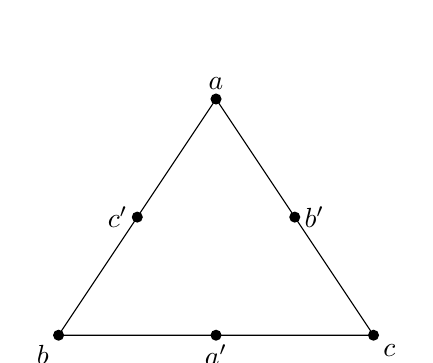
\begin{tikzpicture}
    \coordinate (a) at (0,3);
    \coordinate (b) at (-2,0);
    \coordinate (c) at (2,0);
    \coordinate (a') at ($(b)!0.5!(c)$);
    \coordinate (b') at ($(a)!0.5!(c)$);
    \coordinate (c') at ($(a)!0.5!(b)$);
    \draw (a) -- (b) -- (c) -- cycle;
    \draw (a') -- (a') node[below] {$a'$};
    \draw (b') -- (b') node[right] {$b'$};
    \draw (c') -- (c') node[left] {$c'$};
    \node[above] at (a) {$a$};
    \node[below left] at (b) {$b$};
    \node[below right] at (c) {$c$};
    \foreach \p/\name in {a/a, b/b, c/c, a'/a', b'/b', c'/c'} {
        \fill (\p) circle (2pt); % black dot
    }
  \end{tikzpicture}
  \end{center}
  Set $\triangle_0^1 := \triangle(a,c',b')$,
  $\triangle_0^2 := \triangle(c',b,a')$,
  $\triangle_0^3 := \triangle(a',c,b')$,
  $\triangle_0^4 := \triangle(a',b',c')$.
  \begin{center}
  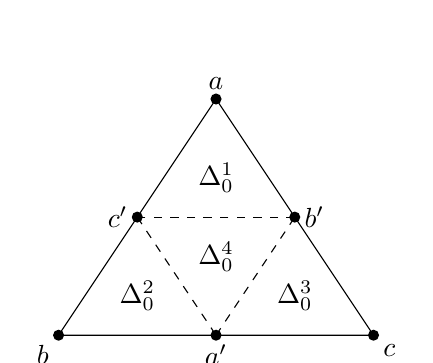
\begin{tikzpicture}
    \coordinate (a) at (0,3);
    \coordinate (b) at (-2,0);
    \coordinate (c) at (2,0);
    \coordinate (a') at ($(b)!0.5!(c)$);
    \coordinate (b') at ($(a)!0.5!(c)$);
    \coordinate (c') at ($(a)!0.5!(b)$);
    \draw (a) -- (b) -- (c) -- cycle;
    \draw (a') -- (a') node[below] {$a'$};
    \draw (b') -- (b') node[right] {$b'$};
    \draw (c') -- (c') node[left] {$c'$};
    \draw (0,2) node {$\triangle_0^1$};
    \draw (-1,0.5) node {$\triangle_0^2$};
    \draw (1,0.5) node {$\triangle_0^3$};
    \draw (0,1) node {$\triangle_0^4$};
    \draw[dashed] (a') -- (b');
    \draw[dashed] (b') -- (c');
    \draw[dashed] (c') -- (a');
    \node[above] at (a) {$a$};
    \node[below left] at (b) {$b$};
    \node[below right] at (c) {$c$};
    \foreach \p/\name in {a/a, b/b, c/c, a'/a', b'/b', c'/c'} {
        \fill (\p) circle (2pt); % black dot
    }
  \end{tikzpicture}
  \end{center}
  We now have that
  \[
    J = \sum_{j=1}^{4} \int_{\ptriangle_0^j} f(z) \dz.
  \]
  Thus, by the triangle inequality there exists $1 \le i \le 4$ so that
  \[
    \abs{J} \le 4 \abs{\int_{\ptriangle_0^j} f(z) \dz}.
  \]
  We can now set $\triangle_1 := \triangle_0^j$ and repeat the preceding
  argument with $\triangle_1$ instead of $\triangle_0$, which generates
  a sequence of closed triangles $\set{\triangle_n}_{n \geq 0}$ so that
  for each $n \geq 0$ we have that
  \[
    \triangle_{n+1} \subset \triangle_{n} \tand
    \diam(\triangle_n) = 2^{-n} D \tand
    \length(\ptriangle_n) = 2^{-n} L
  \]
  and also
  \[
    \abs{J} \le 4^n \abs{\int_{\ptriangle_n} f(z) \dz}.
  \]
  By Cantor's intersection lemma, there exists a unique $z_0 \in \C$ so
  that $\cap_{n \geq 0} \triangle_n = \set{z_0}$.
  Now since $z_0 \in \triangle_0 \subset \Omega \setminus \set{p}$,
  the function $f$ is holomorphic at $z_0$,
  so for every $\epsilon > 0$ there exists $r > 0$ so that
  $D_r(z_0) \subset \Omega$ and
  \[
    \abs{f(z) - f(z_0) - (z - z_0) f'(z_0)} \le
    \epsilon |z - z_0|
  \]
  for all $z \in D_r(z_0)$.
  Since $\diam(\triangle_n) \to 0$ as $n \to \infty$ there exists
  $n \geq 1$ so that $\triangle_n \subset D_r(z_0)$.
  Then for every $z \in \triangle_n$ we have
  \[
    \abs{f(z) - f(z_0) - (z - z_0) f'(z_0)} \le
    \epsilon |z - z_0| \le
    \epsilon \cdot \diam(\triangle_n) = \epsilon 2^{-n} D.
  \]
  Since $- f(z_0) - (z - z_0) f'(z_0)$ is a polynomial from
  \Cref{cor:int-of-pol-is-zero} we can write that
  \[
    \int_{\ptriangle_n} f(z) \dz =
    \int_{\ptriangle_n} f(z) - f(z_0) - (z - z_0) f'(z_0) \dz.
  \]
  From the estimation lemma (\Cref{prop:pathint-bound}) we now have
  that
  \[
    \abs{\int_{\ptriangle_n} f(z) \dz} \le
    \epsilon 2^{-n} D \cdot \length(\ptriangle_n) =
    \epsilon 4^{-n} D L.
  \]
  Using the inequality from earlier
  \[
    \abs{J} \le 4^n \abs{\int_{\ptriangle_n} f(z) \dz} \implies
    \abs{J} \le \epsilon D L.
  \]
  Since this inequality holds for any $\epsilon > 0$ this implies
  that $J = 0$ which completes the proof for the case $p \notin \triangle$.

  Next suppose that $p \in \set{a,b,c}$.
  Without loss of generality assume that $p = a$.
  We then let $0 < t < 1$ be some small value and set
  $w := t b + (1 - t) a$ and $\eta := t c + (1 - t) a$
  as can be seen in the following diagram.
  \begin{center}
  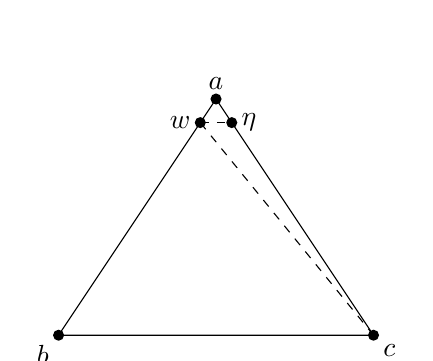
\begin{tikzpicture}
    \coordinate (a) at (0,3);
    \coordinate (b) at (-2,0);
    \coordinate (c) at (2,0);
    \coordinate (w) at ($(a)!0.1!(b)$);
    \coordinate (eta) at ($(a)!0.1!(c)$);
    \draw (a) -- (b) -- (c) -- cycle;
    \draw (w) -- (w) node[left] {$w$};
    \draw (eta) -- (eta) node[right] {$\eta$};
    \draw[dashed] (w) -- (eta);
    \draw[dashed] (c) -- (w);
    \node[above] at (a) {$a$};
    \node[below left] at (b) {$b$};
    \node[below right] at (c) {$c$};
    \foreach \p/\name in {a/a, b/b, c/c, w/w, eta/eta} {
        \fill (\p) circle (2pt); % black dot
    }
  \end{tikzpicture}
  \end{center}
  We now have that
  \[
    J =
    \int_{\ptriangle(a,w,\eta)} f(z) \dz +
    \int_{\ptriangle(w,b,c)} f(z) \dz +
    \int_{\ptriangle(w,c,\eta)} f(z) \dz.
  \]
  Moreover, since $p \notin \triangle(w,b,c)$ and
  $p \notin \triangle(w,c,\eta)$ by the previous result
  \[
    \int_{\ptriangle(w,b,c)} f(z) \dz =
    \int_{\ptriangle(w,c,\eta)} f(z) \dz = 0.
  \]
  Thus we finally have by the estimation lemma
  \[
    \abs{J} =
    \abs{\int_{\ptriangle(a,w,\eta)} f(z) \dz} \le
    \norm{f}_{\triangle} \cdot \length(\ptriangle(a,w,\eta)).
  \]
  Since $f$ is continuous on $\triangle(a,b,c)$ the value of
  $\norm{f}_{\triangle}$ is finite,
  and since this holds for any $t > 0$ and
  $\length(\ptriangle(a,w,\eta)) \to 0$ as $t \to 0$
  we get that $J = 0$ in this case as well.

  Finally, assume that $p \in \triangle \setminus \set{a,b,c}$.
  We then have a triangle of the form
  \begin{center}
  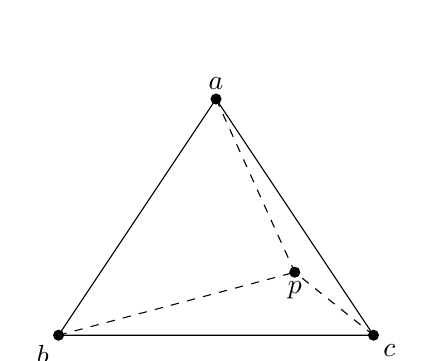
\begin{tikzpicture}
    \coordinate (a) at (0,3);
    \coordinate (b) at (-2,0);
    \coordinate (c) at (2,0);
    \coordinate (p) at (1,0.8);
    \draw (a) -- (b) -- (c) -- cycle;
    \draw (p) -- (p) node[below] {$p$};
    \draw[dashed] (a) -- (p);
    \draw[dashed] (b) -- (p);
    \draw[dashed] (c) -- (p);
    \node[above] at (a) {$a$};
    \node[below left] at (b) {$b$};
    \node[below right] at (c) {$c$};
    % \node[below right] at (c) {$c$};
    \foreach \p/\name in {a/a, b/b, c/c, p/p} {
        \fill (\p) circle (2pt); % black dot
    }
  \end{tikzpicture}
  \end{center}
  and since by the previous case
  \[
    0 =
    \int_{\ptriangle(a,b,p)} f(z) \dz =
    \int_{\ptriangle(b,c,p)} f(z) \dz =
    \int_{\ptriangle(c,a,p)} f(z) \dz,
  \]
  and since $J$ is the sum of these three integrals,
  we get that $J = 0$ which completes the proof of this theorem.
\end{proof}

\subsection{Cauchy's theorem in a convex set}
\begin{theorem}[Cauchy's theorem in a convex set]
  \label{thm:cauchy-convex}
  Let $\Omega \subset \C$ be convex and open,
  let $p \in \Omega$,
  and let $f \colon \Omega \to \C$.
  Suppose that $f$ is continuous on $\Omega$ and holomorphic on
  $\Omega \setminus \set{p}$.
  Then $f$ has a primitive on $\Omega$, and $\int_{\gamma} f(z) \dz = 0$
  for every closed path $\gamma \colon [a,b] \to \Omega$.
\end{theorem}
\begin{proof}
  By \Cref{cor:zero-int} it suffices to show that $f$ has a primitive
  on $\Omega$.
  Fix $z_0 \in \Omega$, and define $F \colon \Omega \to \C$ as such
  \[
    F(z) := \int_{[z_0,z]} f(z) \dz.
  \]
  Since $\Omega$ is convex this function is well define.
  We will show that $F$ is a primitive for $f$ on $\Omega$.
  Let $z_1 \in \Omega$ and $\epsilon > 0$ be given.
  Since $f$ is continuous at $z_1$ there exists $\delta > 0$ such
  that $|f(z) - f(z_1)| < \epsilon$ for all $z \in D_{\delta}(z_1)$.
  Let $0 \neq h \in D_{\delta}(0)$,
  we then have that
  \begin{align*}
    F(z_1 + h) - F(z_1) &=
    \int_{[z_0,z_1 + h]} f(z) \dz + \int_{[z_0,z_1 + h]} f(z) \dz \\ &=
    \int_{\ptriangle(z_0,z_1+h,z_1)} f(z) \dz +
    \int_{[z_1 + h,z_1]} f(z) \dz \\ &=
    \int_{[z_1,z_1+h]} f(z) \dz.
  \end{align*}
  where the last equality follows from \Cref{thm:cauchy-triangle}.
  Moreover, from \Cref{exm:integral-over-interval} we get that
  \[
    \frac{1}{h} \int_{[z_1,z_1+h]} f(z_1) \dz =
    \frac{1}{h} f(z_1) \int_{0}^{1} h \dt = f(z_1).
  \]
  Now since $[z_1,z_1+h] \subset D_{\delta}(z_1)$ we get
  \begin{align*}
    \abs{\frac{F(z_1 + h) - F(z_1)}{h} - f(z_1)} &=
    \abs{\frac{1}{h} \int_{[z_1,z_1+h]} f(z) - f(z_1) \dz} \\ &<
    |h|^{-1} \length\del{[z_1,z_1+h]} \epsilon = \epsilon.
  \end{align*}
  This shows that $F$ is holomorphic at $z_1$ with $F'(z_1) = f(z_1)$,
  which completes the proof of this theorem.
\end{proof}
\begin{remark}
Here are some applications for Cauchy's theorem in a convex set.
\end{remark}
\begin{example}
  We will show that for $\xi \in \R$ we have
  \[
    e^{- \pi \xi^2} =
    \int_{\ninfty}^{\infty} e^{- \pi x^2} e^{2 \pi i x \xi} \dx.
  \]
  This means that $x \mapsto e^{- \pi x^2}$ is its own Fourier transform.
  
  Recall that by using polar coordinates we get
  \[
    \del{\int_{\ninfty}^{\infty} e^{-x^2} \dx}^2 =
    \int_{\ninfty}^{\infty} e^{- x^2 - y^2} \dx \dy =
    \int_{0}^{2 \pi} \int_{0}^{\infty} e^{-r^2} r \dr \dtheta = \pi.
  \]
  This gives that
  \[
    \int_{\ninfty}^{\infty} e^{- \pi x^2} \dx = 1,
  \]
  which shows the result for $\xi = 0$.
% To be added
\end{example}
\begin{example}[Index in squares]
  Let $S_r$ denote the closed square with edges of size $2r$ centered around
  the origin.
  The following is a diagram of its circumference.
\begin{center}
  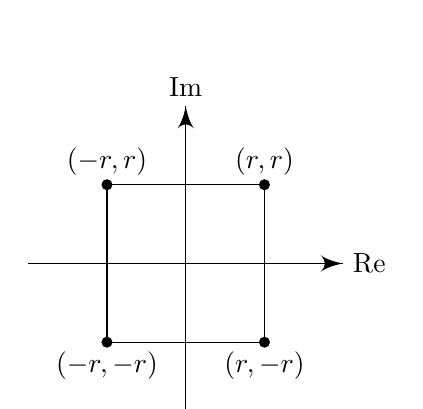
\begin{tikzpicture}
    \draw [->] (-2, 0) -- (2, 0) node [right] {Re};
    \draw [->] (0, -2) -- (0, 2) node [above] {Im};
    \coordinate (a) at (1,1);
    \coordinate (b) at (-1,1);
    \coordinate (c) at (-1,-1);
    \coordinate (d) at (1,-1);
    \node[above] at (a) {$(r,r)$};
    \node[above] at (b) {$(-r,r)$};
    \node[below] at (c) {$(-r,-r)$};
    \node[below] at (d) {$(r,-r)$};
    \draw (a) -- (b) -- (c) -- (d) -- cycle;
    \foreach \p/\name in {a/a, b/b, c/c, d/d} {
        \fill (\p) circle (2pt); % black dot
    }
  \end{tikzpicture}
\end{center}
  Then let $r$, $g$, $b$ and $w$ be the closed red, green, blue and white
  paths in the diagram below.
  Each path starts from a vertice of the square then
  goes over a quarter of $C_{\sqrt{2r}}$ then over the natural edge
  that closes the path.
\begin{center}
  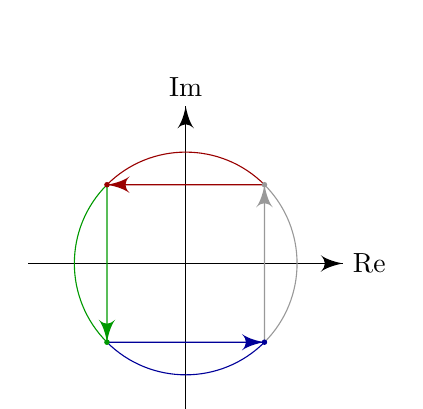
\begin{tikzpicture}
    \draw [->] (-2, 0) -- (2, 0) node [right] {Re};
    \draw [->] (0, -2) -- (0, 2) node [above] {Im};
    \coordinate (a) at (1,1);
    \coordinate (b) at (-1,1);
    \coordinate (c) at (-1,-1);
    \coordinate (d) at (1,-1);
    \node[above,white] at (a) {};
    \node[above,red] at (b) {};
    \node[below,green] at (c) {};
    \node[below,blue] at (d) {};
    
    \draw[black!40!red,->] (a) -- (b) arc[start angle=135, end angle=45, radius={sqrt(2)}] -- (b);
    \draw[black!40!green,->] (b) -- (c) arc[start angle=225, end angle=135, radius={sqrt(2)}] -- (c);
    \draw[black!40!blue,->] (c) -- (d) arc[start angle=315, end angle=225, radius={sqrt(2)}] -- (d);
    \draw[black!40!white,->] (d) -- (a) arc[start angle=45, end angle=-45, radius={sqrt(2)}] -- (a);

    \fill[black!40!white] (a) circle (1pt); % black dot
    \fill[black!40!red] (b) circle (1pt); % black dot
    \fill[black!40!green] (c) circle (1pt); % black dot
    \fill[black!40!blue] (d) circle (1pt); % black dot
  \end{tikzpicture}
\end{center}
  Denote $\gamma$ the closed path that goes over the circumference of the
  square.
  We now have that
  \[
    \int_{r} \frac{\dz}{z - z_0} +
    \int_{g} \frac{\dz}{z - z_0} +
    \int_{b} \frac{\dz}{z - z_0} +
    \int_{w} \frac{\dz}{z - z_0} =
    \int_{\gamma} \frac{\dz}{z - z_0} -
    \int_{C_{\sqrt{2r}}} \frac{\dz}{z - z_0}.
  \]
  However, from \Cref{thm:cauchy-convex} we get that all the integral
  on the left hand side are equal to zero, which means that
  \[
    \Ind_{\gamma}(z_0) =
    \frac{1}{2 \pi i} \int_{\gamma} \frac{\dz}{z - z_0} =
    \frac{1}{2 \pi i} \int_{C_{\sqrt{2r}}} \frac{\dz}{z - z_0}.
  \]
  This means that $\Ind_{\gamma}(z_0) = 1$ if and only if $z_0 \in \Int(S_r)$
  and $\Ind_{\gamma}(z_0) = 0$ when $z_0 \in \C \setminus S_r$.
\end{example}

\subsection{Cauchy's formula in a convex set and its applications}
\begin{theorem}[Cauchy's formula in a convex set]
  \label{thm:cauchy-formula}
  Let $\Omega \subset \C$ be convex and open,
  let $\gamma \colon [a,b] \to \Omega$ be a closed path,
  and let $f \colon \Omega \to \C$ be holomorphic.
  Then for all $z_0 \in \Omega \setminus \gamma^*$ we have
  \[
    f(z_0) \cdot \Ind(z_0) =
    \frac{1}{2 \pi i} \int_{\gamma} \frac{f(z)}{z - z_0} \dz.
  \]
\end{theorem}
\begin{proof}
  Fix $z_0 \in \Omega \setminus \gamma^*$.
  Let $g \colon \Omega \to \C$ be with
  \[
    g(z) :=
    \begin{cases}
      \frac{f(z) - f(z_0)}{z - z_0}, & z \in \Omega \setminus{z_0} \\
      f'(z_0), & z = z_0
    \end{cases}.
  \]
  Since $f$ is holomorphic on $\Omega$, the function $g$ is continuous on
  $\Omega$ and holomophic on $\Omega \setminus \set{z_0}$.
  Thus by Cauchy's theorem on a convex set we have
  \[
    0 =
    \frac{1}{2 \pi i} \int_{\gamma} g(z) \dz =
    \frac{1}{2 \pi i} \int_{\gamma} \frac{f(z) - f(z_0)}{z - z_0} \dz.
  \]
  This implies that
  \[
    \frac{1}{2 \pi i} \int_{\gamma} \frac{f(z)}{z - z_0} \dz =
    f(z_0) \frac{1}{2 \pi i} \int_{\gamma} \frac{1}{z - z_0} \dz =
    f(z_0) \cdot \Ind_{\gamma}(z_0)
  \]
  where the last inequality follows from the definition of
  $\Ind_{\gamma}(z_0)$.
\end{proof}

\begin{remark}
  \label{rmk:cauchy-formula}
  \Cref{thm:cauchy-formula} tells us that the value of $f(z_0)$
  is determined completely
  by the values of $f(z)$ on any closed curve around $z_0$.
\end{remark}

\begin{corollary}[Cauchy's formula]
  \label{cor:f-described-with-integral}
  Let $\Omega \subset \C$ be open,
  let $f \colon \Omega \to \C$ be holomorphic,
  and let $z_0 \in \Omega$ and $r > 0$ be with
  $\overline D_r(z_0) \subset \Omega$.
  Then,
  \[
    f(w) = \frac{1}{2 \pi i} \int_{C_r(z_0)} \frac{f(z)}{z - w} \dz
  \]
  for all $w \in D_r(z_0)$.
\end{corollary}
\begin{proof}
  Since $\Omega$ is open and $\overline C_r(z_0)$ is compact,
  there exists $r' > r$ such that $D_{r'}(z_0) \subset \Omega$.
  Fix $w \in D_r(z_0)$ and let $\gamma$ be the positively oriented circle
  with center $z_0$ and radius $r$.
  Since $D_{r'}(z_0)$ is open and convex and $f$ is holomorphic on
  $D_{r'}(z_0)$ then by Cauchy's formula we get
  \[
    f(w) \cdot \Ind(w) =
    \frac{1}{2 \pi i} \int_{C_r(z_0)} \frac{f(z)}{z - w} \dz.
  \]
  However, since $w \in C_r(z_0)$ we get from an earlier result
  that $\Ind(w) = 1$ and thus
  \[
    f(w) = \frac{1}{2 \pi i} \int_{C_r(z_0)} \frac{f(z)}{z - w} \dz
  \]
  which completes the proof.
\end{proof}

\begin{lemma}
  \label{lem:nderivative}
  Let $\gamma \colon [a,b] \to \C$ be a path,
  let $f_1,f_2,\dots \colon \gamma^* \to \C$ be continuous functions
  and suppose that $f_n \taking{n \to \infty} f$ uniformly on $\gamma^*$
  (i.e.\ $\norm{f - f_n}_{\gamma^*} \to 0$ as $n \to \infty$).
  Then $\int_{\gamma} f_n \dz \taking{n \to \infty} \int_{\gamma} f \dz$.
\end{lemma}
\begin{proof}
  \begin{align*}
    \limsup_{n \to \infty}
    \abs{\int_{\gamma} f(z) \dz - \int_{\gamma} f_n(z) \dz} &=
    \limsup_{n \to \infty} \abs{\int_{\gamma} (f_n - f)(z) \dz} \\ &\le
    \limsup_{n \to \infty} \abs{f_n - f}_{\gamma^*} \cdot \length(\gamma) = 0.
  \end{align*}
\end{proof}

\begin{theorem}
  \label{thm:nderivative}
  Let $\Omega \subset \C$ be open and let $f \colon \Omega \to \C$ be
  holomorphic.
  Then $f$ has infinitely many complex derivatives in $\Omega$.
  Moreover, given $z_0 \in \Omega$ and $r > 0$ with
  $\overline D_r(z_0) \subset \Omega$,
  for all $n \geq 0$ we have
  \[
    f^{(n)}(w) =
    \frac{n!}{2 \pi i} \int_{C_r(z_0)} \frac{f(z)}{(z - w)^{n+1}} \dz
  \]
  for all $w \in D_r(z_0)$, where $f^{(n)}$ denotes the $n$th complex
  derivative of $f$.
\end{theorem}
\begin{proof}
  Let $z_0 \in \Omega$ and $r > 0$ be with $\overline D_r(z_0) \subset \Omega$.
  The proof will be carried out using induction on $n$.
  For $n = 0$ the equality follows directly from
  \Cref{cor:f-described-with-integral}.

  Let $n \geq 1$ and suppose that the equality holds for $n - 1$.
  Fix $w \in D_r(z_0)$ and let $\delta > 0$ be with
  $B_{\delta}(w) \subset D_r(z_0)$.
  For $h \in D_{\delta}(0)$ we get
  \[
    \frac{f^{(n-1)}(w + h) - f^{(n-1)}(w)}{h} =
    \frac{(n-1)!}{2 \pi i}
    \int_{C_r(z_0)} f(z) \frac{1}{h}
    \del{
      \frac{1}{(z - w - h)^{n}} -
      \frac{1}{(z - w)^{n}}
    } \dz.
  \]
  Using the formula for $\alpha, \beta \in \C$,
  \[
    \alpha^n - \beta^n =
    (\alpha - \beta) \sum_{k=0}^{n-1} \alpha^{n - 1 - k} \beta^{k}
  \]
  with $h \in D_{\delta}(0)$ and $z \in C_r(z_0)$ we get
  \[
    \frac{1}{h}
    \del{
      \frac{1}{(z - w - h)^{n}} -
      \frac{1}{(z - w)^{n}}
    } =
    \sum_{k=0}^{n-1} \frac{1}{(z - w - h)^{n-k} (z - w)^{k+1}}.
  \]
  From arithmetics we also get that
  \[
    \lim_{h \to 0} \sup_{z \in C_r(z_0)}
    \abs{
      \sum_{k=0}^{n-1}
      \frac{1}{(z - w - h)^{n-k} (z - w)^{k+1}} - \frac{n}{(z-w)^{n+1}}
    } = 0.
  \]
  Note that $n / (z - w)^{n+1}$ is not part of the sum.
  From the above and \Cref{lem:nderivative} we get
  \[
    \lim_{h \to 0} \frac{f^{(n-1)}(w + h) - f^{(n-1)}(w)}{h} =
    \frac{(n-1)!}{2 \pi i} \int_{C_r(z_0)} f(z) \frac{n}{(z - w)^{n+1}} \dz,
  \]
  which completes the proof of the theorem.
\end{proof}

\begin{corollary}[Cauchy inequalities]
  Let $\Omega \subset \C$ be open,
  let $f \colon \Omega \to \C$ be holomorphic,
  and let $z_0 \in \Omega$ and $r > 0$ be with
  $\overline C_r(z_0) \subset \Omega$.
  Then
  \[
    \abs{f^{(n)}(z_0)} \le
    \frac{n! \norm{f}_{C_r(z_0)}}{r^n}
  \]
  for all $n \geq 0$, where
  $\norm{f}_{C_r(z_0)} = \sup\set{\abs{f(z)} \colon z \in C_r(z_0)}$.
\end{corollary}
\begin{proof}
  By \Cref{thm:nderivative} and \Cref{prop:pathint-bound} we get that
  \begin{align*}
    \abs{f^{(n)}(z_0)} &=
    \abs{\frac{n!}{2 \pi i} \int_{C_r(z_0)} \frac{f(z)}{(z - z_0)^{n+1}} \dz} \\
                       &\le
    \frac{n!}{2 \pi} \cdot
    \length(C_r(z_0)) \cdot 
    \sup_{z \in C_r(z_0)} \abs{\frac{f(z)}{(z - z_0)^{n+1}}} \\ &=
    n! \cdot r \cdot
    \sup_{z \in C_r(z_0)} \abs{\frac{f(z)}{(z - z_0)^{n+1}}} \\ &=
    \frac{n! \norm{f}_{C_r(z_0)}}{r^n}.
  \end{align*}
\end{proof}

\begin{remark}
The following corollary might be one of the most surprising results
in this course.
\end{remark}

\begin{corollary}[Liouville's theorem]
  Let $f \colon \C \to \C$ be entire and bounded.
  Then $f$ is constant.
\end{corollary}
\begin{proof}
  According to \Cref{cor:zero-der-implies-const} it suffices to show
  that $f'(z_0) = 0$ for all $z_0 \in \C$.
  Let $z_0 \in \C$
  and since $f$ is bounded let $C > 1$ be with $\abs{f(z)} \le C$
  for all $z \in \C$.
  According to Cauchy's inequalities it follows that for every $R > 1$
  \[
    \abs{f'(z_0)} \le
    \frac{\norm{f}_{C_R(z_0)}}{R} \le
    \frac{C}{R}.
  \]
  Since this holds for each $\R > 1$ it follows that $f'(z_0) = 0$
  which completes the proof.
\end{proof}
\begin{remark}
  We chose $R > 1$ because this way the results follow more naturally,
  but according to Cauchy's inequalities this of course holds for
  any $R > 0$ as well.
\end{remark}

\begin{corollary}[Fundamental theorem of algebra]
  Let $p(z) = \sum_{k=0}^{n} a_k z^k$ be a nonconstant polynomial with complex
  coefficients.
  Then $p$ has a root in $\C$.
\end{corollary}
\begin{proof}
  Assume by contradiction that $p$ has no root in $\C$.
  Then $f := 1 / p$ is an entire function.
  Since $p$ is nonconstant we have $n \geq 1$ (so that $a_n \neq 0$)
  and thus
  \[
    \liminf_{\abs{z} \to \infty} \abs{p(z)} \geq
    \liminf_{\abs{z} \to \infty} \abs{z}^{n}
    \del{\abs{a_n} - \sum_{k=0}^{n-1} \abs{a_k} \cdot \abs{z}^{k-n}} = \infty.
  \]
  Note that the power is $k - n$ because we factorized $z^n$.
  This means $\abs{z}^{k - n} \taking{\abs{z} \to \infty} 0$ which is
  why the eqality at the end holds.
  In praticular, this equality means that there exists $R > 1$ so that
  $\abs{p(z)} \geq 1$ for all $z \in \C \setminus D_R(0)$ which implies that
  $\abs{f(z)} \le 1$ for all $z \in \C \setminus D_R(0)$.
  Since $f$ is continuous and $\overline D_R(0)$ is compact,
  we have that $\norm{f}_{\overline D_R(0)} < \infty$.
  We have shown that $f$ is an entire and bounded function,
  so by Liouville's theorem it is constant, which implies that
  $p$ is constant which is a contradiction to our assumption.
  This means that our assumption is false and $p$ has a root in $\C$
  which completes the proof.
\end{proof}

\begin{corollary}
  Let $n \geq 1$ and let $p(z) = \sum_{k=0}^{n} a_k z^k$ be a polynomial
  of degree $n$ with complex coefficients.
  Then there exists $w_1,\dots,w_n \in \C$ such that
  \[
    p(z) = a_n \prod_{k=1}^{n} (z - w_k).
  \]
\end{corollary}
\begin{proof}
  We prove this corollary by induction.
  For the base case $n = 1$ we let $w_1 := a_0 / a_1$ and then the claim
  holds.
  Suppose that the claim holds for $n - 1$ and let
  $p(z) = \sum_{k=0}^{n} a_k z^k$ by a polynomial of degree $n$.
  From the fundamental theorem of algebra there exists $w_n \in \C$ so
  that $p(w_n) = 0$, and from polynomial long division there exists
  a polynomial $q(z) = \sum_{k=0}^{n-1} b_k z^k$ of degree $n - 1$
  so that $p(z) = (z - w_n) q(z) + c$.
  We also get that $c = 0$ since
  \[
    0 = p(w_n) = (w_n - w_n) q(w_n) + c = c
  \]
  so $p(z) = (z - w_n) q(z)$.
  This implies that $a_n = b_{n-1}$.
  From this, and from the induction hypothesis, there exist
  $w_1,\dots,w_{n-1} \in \C$ so that
  \[
    q(z) = a_n \prod_{k=1}^{n-1} (z - w_k).
  \]
  This implies that
  \[
    p(z) = (z - w_n) q(z) = (z - w_n) a_n \prod_{k=1}^{n-1} (z - w_k),
  \]
  which completes the proof of this corollary.
\end{proof}

\subsection{The analyticity of holomorphic functions}

\begin{remark}
We have already seen that an analytic function on an open set
$\Omega \subset \C$ is holomorphic on that set.
We now use Cauchy's formula to prove the converse.
\end{remark}

\begin{theorem}
  \label{thm:holomorphic-implies-analytic}
  Let $\Omega \subset \C$ be open,
  let $f \colon \Omega \to \C$ be holomorphic,
  let $z_0 \in \Omega$,
  and let $R > 0$ be with $D_R(z_0) \subset \Omega$.
  Then $f(z) = \sum_{n=0}^{\infty} a_n (z - z_0)^n$
  for all $z \in D_R(z_0)$,
  where $a_n := f^{(n)}(z_0) / n!$ for each $n \geq 0$.
  In particular, $f$ is analytic on $\Omega$.
\end{theorem}
\begin{proof}
  Fix some $z \in D_R(z_0)$ and let $\abs{z - z_0} < r < R$.
  By \Cref{cor:f-described-with-integral}
  \[
    f(z) = \frac{1}{2 \pi i} \int_{C_r(z_0)} \frac{f(w)}{w - z} \dw.
  \]
  For $w \in C_r(z_0)$ we have
  \[
    \frac{1}{w - z} =
    \frac{1}{w - z_0 - (z - z_0)} =
    \frac{1}{w - z_0} \cdot \frac{1}{1 - \frac{z - z_0}{w - z_0}}
  \]
  and
  \[
    \abs{\frac{z - z_0}{w - z_0}} =
    \abs{\frac{z - z_0}{r}} < 1.
  \]
  Therefore by using the geometric series formula we get
  \[
    \frac{1}{w - z} =
    \frac{1}{w - z_0} \sum_{n=0}^{\infty} \del{\frac{z - z_0}{w - z_0}}^{n}
  \]
  and the series converges uniformly for $w \in C_r(z_0)$.
  According to \Cref{lem:nderivative} we now obtain
  \begin{align*}
    f(z) &= \frac{1}{2 \pi i} \int_{C_r(z_0)}
    \frac{f(w)}{w - z_0} \sum_{n=0}^{\infty} \del{\frac{z - z_0}{w - z_0}}^{n} \dw
         \\ &=
         \frac{1}{2 \pi i} \sum_{n=0}^{\infty} \del{(z - z_0)^n
         \int_{C_r(z_0)} \frac{f(w)}{(w - z_0)^{n+1}} \dw}.
  \end{align*}
  This shows that $f$ is analytic.
  Moreover, by \Cref{thm:nderivative}
  \[
    \frac{f^{(n)}(z_0)}{n!} =
    \frac{1}{2 \pi i}
    \int_{C_r(z_0)} \frac{f(w)}{(w - z_0)^{n+1}} \dw
  \]
  for $n \geq 0$ which shows that the coefficients of the power series are
  what we proposed them to be which completes the proof.
\end{proof}
\begin{remark}
  Note that if $f \colon \C \to \C$ is entire then it follows that
  $f(z) = \sum_{n=0}^{\infty} a_n z^n$ for all $z \in C$,
  where $a_n := f^{(n)}(0) / n!$ for each $n \geq 0$.
\end{remark}

\begin{theorem}
  \label{thm:zeros-have-limit-implies-f-is-zero}
  Let $\Omega \subset \C$ be a region and let $f \colon \Omega \to \C$
  be holomorphic.
  Write $Z := \set{z \in \Omega \mid f(z) = 0}$,
  and suppose that $Z$ has a limit point in $\Omega$.
  Then $f(z) = 0$ for all $z \in \Omega$.
\end{theorem}
\begin{proof}
  Denote by $\Omega_1$ the set of limit points of $Z$ in $\Omega$.
  We will show that $\Omega_1$ is an open subset of $\C$.
  Fix $z_0 \in \Omega_1$, and let $\epsilon > 0$ by with
  $D_{\epsilon}(z_0) \subset \Omega$.
  By \Cref{thm:holomorphic-implies-analytic} there exist
  $a_0,a_1,\dots \in \C$ so that $f(z) = \sum_{n=0}^{\infty} a_n (z - z_0)^n$
  for all $z \in D_{\epsilon}(z_0)$.
  Assume by way of contradiction that $a_n \neq 0$ for some $n \geq 1$.
  Then let $m = \min\set{n \in \N \mid a_n \neq 0}$ and denote
  $g(z) = \sum_{n=0}^{\infty} a_{n+m} (z - z_0)^n$.
  Since $g(z_0) = a_m \neq 0$ and $g$ is continuous there exists a
  $0 < \delta < \epsilon$ so that $g(z) \neq 0$ for all $z \in D_{\delta}(z_0)$.
  Since $z_0$ is a limit point of $z$ there exists a point
  $w \in D_{\delta}(z_0)$ so that $f(w) = 0$.
  We now see that since $w \in D_{\delta}(z_0)$ and $w \neq z_0$ that
  $(w - z_0)^m g(w) \neq 0$.
  However, we also have that
  \[
    0 = f(w) =
    \sum_{n=m}^{\infty} a_n (w - z_0)^n =
    (w - z_0)^m g(w).
  \]
  This contradiction implies that $a_n = 0$ for all $n \geq 0$,
  which means that $f(z) = 0$ for all $z \in D_{\epsilon}(z_0)$.
  This implies that $D_{\epsilon}(z_0) \subset Z$,
  which very elegantly implies that $D_{\epsilon}(z_0) \subset \Omega_1$,
  which means that $\Omega_1$ is indeed an open subset of $\C$.

  We now assume by contradiction that $\Omega_2 := \Omega \setminus \Omega_1$
  is nonempty, and fix $z_0 \in \Omega_2$.
  Since $z_0$ is not a limit point of $Z$ there exists $\epsilon > 0$
  so that $D_{\epsilon}(z_0) \subset \Omega$ and $f(z) \neq 0$ for all
  $z \in D_{\epsilon}(z_0) \setminus \set{z_0}$.
  This also elegantly implies that the point in $D_{\epsilon}(z_0)$ are not
  limit points of $Z$, and thus $D_{\epsilon}(z_0) \subset \Omega_2$
  which means that $\Omega_2$ is also an open subset of $\C$.

  Since $\Omega$ is a region, and since $\Omega$ is the disjoint union
  of two open sets $\Omega_1$ and $\Omega_2$,
  this implies that either $\Omega_1 = \emptyset$ or $\Omega_2 = \emptyset$.
  Since by assumption $\Omega_1 \neq \emptyset$ we get that
  $\Omega_2 = \emptyset$ and so $\Omega_1 = \Omega$.
  This means that every $z \in \Omega$ is a limit point of $Z$,
  and since $f$ is continuous it follows that $\Omega = Z$ which completes
  the proof.
\end{proof}

\begin{corollary}
  \label{cor:almost-equal-functions-are-equal}
  Let $\Omega \subset \C$ be a region and let $f,g \colon \Omega \to \C$
  be holomorphic.
  Set $A := \set{z \in \Omega \mid f(z) = g(z)}$,
  and suppose that $A$ has a limit point in $\Omega$.
  Then $f(z) = g(z)$ for all $z \in \Omega$.
\end{corollary}
\begin{proof}
  The proof follows directly from applying
  \Cref{thm:zeros-have-limit-implies-f-is-zero}
  on the function $f - g$.
\end{proof}

\begin{definition}[Analytic continuation]
  Let $\Omega_1, \Omega_2 \in \C$ be regions with $\Omega_1 \subset \Omega_2$.
  For $i = 1, 2$ let $f_i \colon \Omega_i \to \C$ be holomorphic,
  and suppose that $f_1 = f_2$ on $\Omega_1$.
  We say that $f_2$ is an analytic continuation of $f_1$ into the region
  $\Omega_2$.
\end{definition}
\begin{remark}
  From \Cref{cor:almost-equal-functions-are-equal}
  it follows that the analytic continuation of $f_1$ into $\Omega_2$
  is unique.
\end{remark}

\subsection{Further applications}

\begin{theorem}[Morera's theorem]
  Let $\Omega \subset \C$ be open,
  let $f \colon \Omega \to \C$ be continuous,
  and suppose that $\int_{\ptriangle} f \dz = 0$ for every closed triangle
  $\triangle \subset \Omega$.
  Then $f$ is holomorphic on $\Omega$.
\end{theorem}
\begin{proof}
  Since we need to show that $f$ is holomorphic at every $z \in \Omega$,
  and any $z \in \Omega$ is contained in a sufficiently small epsilon ball,
  it suffices to show that $f$ is holomorphic on every open convex subset
  of $\Omega$.
  Let $V \subset \Omega$ be an open convex set.
  Fix $z_0 \in V$, and for $z \in V$ set
  \[
    F(z) := \int_{[z_0,z]} f(w) \dw.
  \]
  In the exact same process from \Cref{thm:cauchy-convex} we can show that
  $F$ is a primitive for $f$ on $V$, and in particular it is holomorphic on $V$.
  By \Cref{lem:nderivative} it follows that complex derivatives of holomorphic
  functions are holomorphic.
  This means that $f = F'$ is holomorphic on $V$ which completes the proof.
\end{proof}

\begin{definition}[Uniform convergence on compact subsets]
  Let $\Omega \subset \C$ and $f,f_1,f_2,\dots \colon \Omega \to \C$ be given.
  We say that $f_n \taking{n \to \infty} f$ uniformly on compact subsets of
  $\Omega$ if for every compact $K \subset \Omega$ we have
  $\norm{f - f_n}_{K} \taking{n \to \infty} 0$.
\end{definition}
\begin{remark}
  \label{rmk:uniform-convergence-continuity}
  Suppose we also know that $\Omega$ is open and that $f_1,f_2,\dots$
  are continuous on $\Omega$.
  Then $f$ is also continuous on $\Omega$.
\end{remark}

\begin{proposition}
  \label{prop:uconvergence-preserves-holomorphicity}
  Let $\Omega \subset \C$ and $f,f_1,f_2,\dots \colon \Omega \to \C$ be given.
  Suppose that $f_n$ is holomorphic on $\Omega$ for each $n \geq 1$,
  and that $f_n \taking{n \to \infty} f$ uniformly on compact subsets of
  $\Omega$.
  Then $f$ is also holomorphic on $\Omega$.
\end{proposition}
\begin{proof}
  Accoridng to \Cref{rmk:uniform-convergence-continuity} it follows that
  $f$ is continuous.
  Let $\triangle \subset \Omega$ be a closed triangle.
  Since $\triangle$ is compact,
  we have $\norm{f - f_n}_{\triangle} \taking{n \to \infty} 0$.
  From \Cref{lem:nderivative} we obtain that
  \[
    \int_{\ptriangle} f_n \dz \taking{n \to \infty} \int_{\ptriangle} f \dz.
  \]
  However, since $f_n$ is holomorphic for $n \geq 1$,
  it follows that every term in the sequence is $0$ which implies
  that $\int_{\ptriangle} f \dz$.
  Thus from Morera's theorem it follows that $f$ is holomorphic on $\Omega$
  which completes the proof.
\end{proof}
\begin{remark}
  This proposition is clearly false in the case of real analysis.
  This is because by the Weierstrass approximation theorem,
  any continuous function on a compact interval can be uniformly approximated
  by polynomials (which are holomorphic), but not every continuous function
  on a compact interval is holomorphic when extended to the complex plane.
\end{remark}

\begin{example}[Riemann zeta function]
  For $r > 0$ and $z \in \C$ we define $z := e^{z \log r}$,
  where $\log$ is the standard real logarithm function.
  Since $z \mapsto e^z$ is entire,
  it follows from arithmetic operations that $z \mapsto r^z$ is also entire.
  For $t > 0$ we define the set
  \[
    H_t := \set{z \in \C \colon \Re(z) > t}.
  \]
  Given $t > 1$ and $z \in H_t$ we have that
  \[
    \sum_{n=1}^{\infty} \abs{\frac{1}{n^z}} =
    \sum_{n=1}^{\infty} \abs{e^{-z \log n}} =
    \sum_{n=1}^{\infty} e^{-\Re(z) \log n} \le
    \sum_{n=1}^{\infty} e^{-t \log n} =
    \sum_{n=1}^{\infty} \frac{1}{n^t} < \infty.
  \]
  From this follows that the function $\zeta \colon H_1 \to \C$ with
  \[
    \zeta(z) := \sum_{n=1}^{\infty} \frac{1}{n^z}
  \]
  is well defined.
  The function $\zeta$ is called the Riemann zeta function.
  We can also show that it is holomorphic on $H_1$.
  Let $t > 1$ be given.
  As we saw previously for $z \in H_t$ and $N \geq 1$ we have
  \[
    \abs{\zeta(z) - \sum_{n=1}^{N} \frac{1}{n^z}} =
    \abs{\sum_{n=N+1}^{\infty} \frac{1}{n^z}} \le
    \sum_{n=N+1}^{\infty} \abs{\frac{1}{n^z}} \le
    \sum_{n=N+1}^{\infty} \frac{1}{n^t} \taking{N \to \infty} 0
  \]
  where the last step follows from $t > 1$.
  This shows the function sequence
  $\set{z \mapsto \sum_{n=1}^{N} \frac{1}{n^z}}_{N \geq 1}$
  converges uniformly to $\zeta$ on $H_t$.
  Thus, since $z \mapsto \sum_{n=1}^{N} \frac{1}{n^z}$ is entire for all
  $N \geq 1$ and from \Cref{prop:uconvergence-preserves-holomorphicity}
  we get that $\zeta$ is holomorphic on $H_t$.
  Since this holds for all $t > 1$,
  we get that $\zeta$ is holomorphic on $H_1$.
\end{example}

\begin{remark}
  There are similar theorems about convergence of sequences of derivatives.
\end{remark}

\begin{theorem}
  Let $\Omega \subset \C$ be open and let $f,f_1,f_2,\dots \colon \Omega \to \C$
  be holomorphic.
  Suppose that $f_n \taking{n \to \infty} f$ uniformly on compact subsets of
  $\Omega$.
  Then for each $k \geq 1$ we have $f^{(k)}_n \taking{n \to \infty} f^{(k)}$
  uniformly on compact subsets of $\Omega$
\end{theorem}
\begin{proof}
  To be added.
\end{proof}

\begin{proposition}
  \label{prop:gamma}
  Let $\Omega \subset \C$ be open
  and let $F \colon \Omega \times [0,1] \to \C$ be continuous on
  $\Omega \times [0,1]$.
  Suppose that for each $s \in [0,1]$ the function $z \mapsto F(z,s)$ is
  holomorphic on $\Omega$.
  Let $f \colon \Omega \to \C$ be with
  \[
    f(z) := \int_{0}^{1} F(z,s) \ds
  \]
  for $z \in \Omega$, then $f$ is holomorphic on $\Omega$.
\end{proposition}
\begin{proof}
  Using \Cref{prop:uconvergence-preserves-holomorphicity}. To be added.
\end{proof}

\begin{example}[Gamma function]
  For each $0 < \epsilon < 1$ let $f_{\epsilon} \colon \C \to \C$ be with
  \[
    f(z) := \int_{\epsilon}^{1/\epsilon} e^{-t} t^{z - 1} \dt,
  \]
  where $t^{z-1} := e^{(z - 1) \log t}$ for $t > 0$.
  By \Cref{prop:gamma} it follows that $f_{\epsilon}$ is entire.
  
  Set $H_0 := \set{z \in \C \colon \Re(z) > 0}$,
  and let $\Gamma \colon H_0 \to \C$ be such that
  \[
    \Gamma(z) := \int_{0}^{\infty} e^{-t} t^{z - 1} \dt.
  \]
  The function $\Gamma$ which is called the gamma function, is well defined.
  Since it can be shows that $f_{1/n} \taking{n \to \infty} \Gamma$ uniformly
  on compact subsets of $H_0$,
  it follows by \Cref{prop:uconvergence-preserves-holomorphicity}
  that $\Gamma$ is holomorphic on $H_0$.
\end{example}

% Remarks about zeta/gamma functions?

\subsection{Harmonic functions}
\begin{definition}[Harmonic function]
  Let $U \subset \C$ be a region and let $u \colon U \to \R$ be a real-valued
  function with $2$nd order partial derivatives.
  Then $u$ is said to be harmonic on $U$ if it satisifes the
  \textit{Laplace equation}:
  \[
    \Delta u = \nabla^2 u = \diffp[2]{u}{x} + \diffp[2]{u}{y} = 0,
  \]
  at any point $p \in U$.
\end{definition}
\begin{remark}
  We say that $u$ is harmonic at $p \in U$ if it satisfies the Laplace
  equation at $u$.
  In some sources, we say that $u$ is harmonic on $U$ if it is harmonic
  at all $u \in \overline U$.
\end{remark}
\begin{remark}
  The Laplace equation is one of the most important partial differential
  equations of mathematical physics.
\end{remark}

\begin{proposition}
  Let $U \subset \C$
  be a region and let $f \colon U \to \C$ so that $f = u + i v$ be holomorphic.
  Then $u$ and $v$ are harmonic functions.
\end{proposition}
\begin{proof}
  Since $f$ is holomorphic, by \Cref{thm:holomorphic-implies-analytic}
  and \Cref{cor:infinitely-differentiable} it is infinitely complex
  differentiable, and thus $u$ and $v$ have continuous $2$nd derivatives.
  From the Cauchy--Riemann equations we get
  \[
    \diffp{u}{x} = \diffp{v}{y} \stand
    \diffp{u}{y} = -\diffp{v}{x}.
  \]
  It follows that
  \begin{align*}
    \Delta u &= \diffp[2]{u}{x} + \diffp[2]{u}{y} \\
        &= \diffp{}{x} \del{\diffp{u}{x}} + \diffp{}{y} \del{\diffp{u}{y}} \\
        &= \diffp{}{x} \del{\diffp{v}{y}} - \diffp{}{y} \del{\diffp{v}{x}} \\
        &= \diffp{}{x} \del{\diffp{v}{y}} - \diffp{}{x} \del{\diffp{v}{y}} \\
        &= 0.
  \end{align*}
  The same argument holds for $v$, which completes the proof.
\end{proof}

\begin{definition}[Harmonic conjugate]
  Let $U \subset \C$ be a region and let $u \colon U \to \R$  be harmonic.
  A harmonic function $v \colon U \to \R$ is called a harmonic conjugate
  of $u$ if $f = u + i v$ is holomorphic.
\end{definition}

\begin{remark}
  Note that if $v$ is a harmonic conjugate of $u$ and $a$ is a complex
  number then $v + a$ is also a harmonic conjugate of $u$ since
  \[
    u + i(v + a) = f + ia
  \]
  is holomorphic.
  On the other hand, if $v$ and $w$ are both harmonic conjugates of $u$,
  then we have
  \[
    i(w - v) = (u + i v) - (u + i w) = f - g
  \]
  which is holomorphic as the difference of two holomorphic functions.
  Since $i(w - v)$ is purely imaginary and holomorphic,
  it must be constant.
  This implies that $w = v + a$ for some complex number $a \in \C$.
  In conclusion, harmonic functions are unique up to addition of a constant.
\end{remark}

\begin{example}
  It is clear that $u = xy$ is harmonic since its second partial derivatives
  are continuous, and we have
  \[
    \Delta u = \nabla^2 u = \diffp[2]{u}{x} + \diffp[2]{u}{y} = 0.
  \]
  In order to find the harmonic conjugate we first need to solve the
  Cauchy--Riemann equations
  \begin{gather*}
    v_y = y, \\
    v_x = -x.
  \end{gather*}
  In order to solve these equations we see that
  \[
    v(x,y) = \frac{y^2}{2} + h(x) + c
  \]
  where $h(x)$ is some function in $x$, and $c$ is some constant.
  Plugging $v(x,y)$ into the second equation gives $h'(x) = -x$ which implies
  \[
     v(x,y) = \frac{y^2}{2} - \frac{x^2}{2} + C.
  \]
  For simplicity we will only consider $v(x,y)$ with $c = 0$.
  We notice that if $f = u + i v$, then we actually have
  \[
    f(z) = i \frac{z^2}{2} + c.
  \]
\end{example}

\begin{proposition}
  \label{prop:harmonic-on-rectangle}
  Let $U$ be an open rectangle with sides parallel to the axes.
  Then every harmonic function $u$ on $U$ has a harmonic conjugate.
\end{proposition}
\begin{proof}
  Let $(x_0,y_0) \in U$.
  We start by integrating the first Cauchy--Riemann equation
  with respect to $y$:
  \[
    v(x,y) = \int_{y_0}^{y} \diffp{u}{x}(x,t) \dt + h(x),
  \]
  where $h(x)$ is the constant of integration (which may depend on $x$).
  We then proceed to plug this into the second Cauchy--Riemann equation:
  \begin{align*}
    \diffp{u}{y}(x,y) &=
    -\diffp{}{x} \int_{y_0}^{y} \diffp{u}{x}(x,t)\dt - h'(x) \\ &=
    -\int_{y_0}^{y} \diffp[2]{u}{x}(x,t)\dt - h'(x) \\ &=
    \int_{y_0}^{y} \diffp[2]{u}{y}(x,t)\dt - h'(x) \\ &=
    \diffp{u}{y}(x,y) - \diffp{u}{y}(x,y_0) - h'(x).
  \end{align*}
  Hence
  \[
    h'(x) = - \diffp{u}{y}(x,y_0).
  \]
  Integrating both sides with respect to $x$ gives
  \[
    h(x) = - \int_{x_0}^{x} \diffp{u}{y} (s,y_0) \ds,
  \]
  up to addition of a constant.
  Thus,
  \[
    v(x,y) =
    \int_{y_0}^{y} \diffp{u}{x}(x,t) \dt -
    \int_{x_0}^{x} \diffp{u}{y} (s,y_0) \ds,
  \]
  up to a constant.
\end{proof}

\begin{proposition}
  Let $U$ be an open disk.
  Then every harmonic function $u$ on $U$ has a harmonic conjugate.
\end{proposition}
\begin{proof}
  We can use the same proof from \Cref{prop:harmonic-on-rectangle},
  except we must choose $(x_0,y_0)$ to be be the center of the disc.
  That is because if we choose another point, the rectangle
  we integrate on could intersect with the space outside the disc.
\end{proof}


\newpage

\section{Meromorphic functions and the logarithm}

\subsection{Zeros and singularties}
\begin{definition}[Zero]
  Let $\Omega \subset \C$ be open and let $f \colon \Omega \to \C$ be
  holomorphic.
  A number $z_0 \in \Omega$ is said to be a zero of $f$ if $f(z_0) = 0$.
\end{definition}

\begin{proposition}
  \label{prp:zero-can-be-removed}
  Let $\Omega \subset \C$ be a region,
  let $f \colon \Omega \to \C$ be holomorphic,
  suppose that $f$ does not vanish identically in $\Omega$,
  and let $z_0$ be a zero of $f$.
  Then there exists a unique integer $m \geq 1$ for which there exists a
  holomorphic $g \colon \Omega \to \C$ so that $g(z_0) \neq 0$ and
  $f(z) = (z - z_0)^m g(z)$ for each $z \in \Omega$.
\end{proposition}
\begin{proof}
  Since a holomorphic function is analytic and $\Omega$ is a region,
  there exists $\epsilon > 0$ and $\set{a_i}_{i=0}^{\infty} \subset \C$
  so that $D_{\epsilon}(z_0) \subset \Omega$ and
  \[
    f(z) = \sum_{n=0}^{\infty} a_n(z - z_0)^n
  \]
  for $z \in D_{\epsilon}(z_0)$.
  Since $f$ does not vanish identically in $\Omega$,
  by \Cref{thm:zeros-have-limit-implies-f-is-zero} it does not vanish
  identically in $D_{\epsilon}(z_0)$.
  Since $f$ is analytic and $f(z_0)$ it follows elegantly
  that there exists $m \geq 1$ so that $a_m \neq 0$ and $a_n = 0$
  for $0 \le n \le m$.
  We now define $g \colon \Omega \to \C$ by
  \[
    g(z) :=
    \begin{cases}
      (z - z_0)^{-m} f(z), &z \in \Omega \setminus \set{z_0} \\
      a_m, &z = z_0
    \end{cases}.
  \]
  It is clear that $f$ is holomorphic on $\Omega \setminus \set{z_0}$.
  By definition we have that
  \[
    g(z) = \sum_{n=0}^{\infty} a_{n+m} (z - z_0)^n
  \]
  for $z \in D_{\epsilon}(z_0)$.
  This means it is analytic and thus holomorphic at $z_0$ so it is holomorphic
  on $\Omega$ and $f(z) = (z - z_0)^{m} g(z)$ for $z \in \Omega$.
  We also note that $g(z_0) = a_m \neq 0$ so it satisfies all required
  properties.

  We still need to show that $m$ is unique.
  Let $k \geq 1$ be an integer for which there exists a
  holomorphic $h \colon \Omega \to \C$ so that $h(z_0) \neq 0$ and
  $f(z) = (z - z_0)^k h(z)$ for each $z \in \Omega$.

  Assume by contradiction that $m < k$.
  Then we obtain $g(z) = (z - z_0)^{k - m} h(z)$
  for $z \in \Omega \setminus \set{z_0}$.
  As $z \to z_0$ we get from continuity of $g$ that $g(z_0) = 0$ which is
  a contradiction to $g(z_0) \neq 0$.
  A similar argument shows that $k < m$ is not possible,
  which completes the proof.
\end{proof}

\begin{definition}[Isolated singularity]
  Let $\Omega \subset \C$ be open,
  let $z_0 \in \Omega$,
  and let $f \colon \Omega \setminus \set{z_0} \to \C$ be holomorphic.
  In this case we say that $f$ has an isolated singularity at $z_0$.
\end{definition}
\begin{remark}[Removable singularity]
  If we can define $f$ at $z_0$ in such a way that $f$ becomes holomorphic
  in all of $\Omega$ then we say that $z_0$ is a removable singularity of $f$.
\end{remark}

\begin{definition}[Punctured disc]
  Given $z_0 \in \C$ and $r > 0$ we denote $D'_r(z_0)$ the punctured open disc
  with center $z_0$ and radius $r$.
  That is
  \[
    D'_r(z_0) := \set{z \in \C \colon 0 < |z - z_0| < r}.
  \]
\end{definition}

\begin{theorem}[Riemann's removable singularity theorem]
  \label{thm:riemann-removable-singularity}
  Let $\Omega \subset \C$ be open,
  let $z_0 \in \Omega$,
  and let $f \colon \Omega \setminus \set{z_0} \to \C$ be holomorphic.
  Suppose that $f$ is bounded in $D'_r(z_0)$ for some $r > 0$.
  Then $z_0$ is a removable singularity of $f$.
\end{theorem}
\begin{proof}
  Let $g \colon \Omega \to \C$ be such that
  \[
    g(z) :=
    \begin{cases}
      0, &z = z_0 \\
      (z - z_0)^2 f(z), &z \in \Omega \setminus \set{z_0}
    \end{cases}.
  \]
  Since $f$ is bounded in $D'_r(z_0)$ we get that
  \[
    \lim_{h \to 0} \frac{g(z_0 + h) - g(z_0)}{h} =
    \lim_{h \to 0} h f(z_0 + h) = 0,
  \]
  which means that $g$ is holomorphic at $z_0$ with $g'(z_0) = 0$.
  Since $g$ is also holomorphic on $\Omega \setminus \set{z_0}$,
  we get in total that $g$ is holomorphic on $\Omega$.
  By \Cref{thm:holomorphic-implies-analytic} we get that $g$ is analytic
  on $\Omega$ and since $g(z_0) = g'(z_0) = 0$, there exists $\epsilon > 0$
  with $D_{\epsilon}(z_0) \subset \Omega$ and $a_2,a_3,\dots \in \C$ so
  that $g(z) = \sum_{n=2}^{\infty} a_n (z - z_0)^n$ for
  $z \in D_{\epsilon}(z_0)$.
  thus for $z \in D'_{\epsilon}(z_0)$ we have
  \[
    f(z) =
    (z - z_0)^{-2} g(z) =
    \sum_{n=2}^{\infty} a_n (z - z_0)^{n-2} =
    \sum_{n=0}^{\infty} a_{n+2} (z - z_0)^{n}.
  \]
  The function on the right hand side is a holomorphic extension of $f$ to
  $D_{\epsilon}(z_0)$ which means that by setting $f(z_0) := a_2$
  we get the desired result which completes the proof.
\end{proof}
\begin{remark}
  The above theorem is sometimes called Riemann's theorem,
  and it actually states that the following are equivalent
  \begin{enumerate}
    \item[(1)] $f$ is holomorphically extendable over $z_0$.
    \item[(2)] $f$ is continuously extendable over $z_0$.
    \item[(3)] There exists a neighbourhood of $a$ in which $f$ is bounded.
    \item[(4)] $\lim_{z \to z_0} (z - z_0) f(z) = 0$.
  \end{enumerate}
\end{remark}

\begin{definition}[Pole]
  Let $\Omega \subset \C$ be open,
  let $z_0 \in \Omega$,
  and let $f \colon \Omega \setminus \set{z_0} \to \C$ be holomorphic.
  We say that $f$ has a pole at $z_0$ if there exists $\epsilon > 0$
  such that $D_{\epsilon}(z_0) \subset \Omega$ and $f(z) \neq 0$ for
  $z \in D'_{\epsilon}(z_0)$, and the function
  \[
    g(z) :=
    \begin{cases}
      \frac{1}{f(z)}, &\text{for } z \in D'_{\epsilon}(z_0) \\
      0, &\text{for } z = z_0
    \end{cases}
  \]
  is holomorphic on $D_{\epsilon}(z_0)$.
\end{definition}
\begin{remark}
  Note that if $f$ has a pole at $z_0$ then
  $\lim_{z \to z_0} \abs{f(z)} = \infty$.
  We will see later that this is an if and only if statement.
\end{remark}

\begin{proposition}
  \label{prop:order-of-the-pole}
  Let $\Omega \subset \C$ be open,
  let $z_0 \in \Omega$,
  let $f \colon \Omega \setminus \set{z_0} \to \C$ be holomorphic,
  and suppose that $f$ has a pole at $z_0$.
  Then there exists a unique integer $m \geq 1$ for which there exists
  $\delta > 0$ with $D_{\delta}(z_0) \subset \Omega$ and a holomorphic
  $g \colon D_{\delta}(z_0) \to \C$ such that $g(z) \neq 0$ and
  $f(z) = (z - z_0)^{-m} g(z)$ for $z \in D'_{\delta}(z_0)$.
\end{proposition}
\begin{remark}
  The integer $m$ is called the order of the pole which $f$ has at $z_0$.
\end{remark}
\begin{remark}[Simple pole]
  If the order of is pole is $m = 1$, we say that it is a simple pole.
\end{remark}
\begin{proof}
  To be added.
\end{proof}

\begin{proposition}
  \label{prop:almost-loren}
  Let $\Omega \subset \C$ be open,
  let $z_0 \in \Omega$,
  let $f \colon \Omega \setminus \set{z_0} \to \C$ be holomorphic,
  and suppose that $f$ has a pole of order $m$ at $z_0$.
  Then there exists $\epsilon > 0$ with $D_{\epsilon}(z_0) \subset \Omega$
  and $a_{-m},a_{-m+1},\dots,a_{-1} \in \C$ with $a_{-m} \neq 0$,
  and a holomorphic $h \colon D_{\epsilon}(z_0) \to \C$, such that
  \[
    f(z) =
    \frac{a_{-m}}{(z - z_0)^{m}} + \cdots +
    \frac{a_{-1}}{(z - z_0)} + h(z)
  \]
  for $z \in D'_{\epsilon}(z_0)$.
\end{proposition}
\begin{remark}
  The sum $\frac{a_{-m}}{(z - z_0)^{m}} + \cdots + \frac{a_{-1}}{(z - z_0)}$
  is called the \textit{principle part} of $f$ at the pole $z_0$,
  and the coefficient $a_{-1}$ is called the residue of $f$ at that
  pole.
  We shall write $\Res(f,z_0)$ instead of $a_{-1}$.
  The importance of the residue comes from the fact that
  all the other terms in the principle part have primitives in
  a deleted neighbourhood of $z_0$.
  This will be extreamly helpful for us later when we will talk about
  the residue theorem.
\end{remark}
\begin{proof}
  Since $f$ has a pole of order $m$ at $z_0$, there exists
  $\epsilon > 0$ with $D_{\epsilon}(z_0) \subset \Omega$ and a holomorphic
  $g \colon D_{\epsilon}(z_0) \to \C$ such that $g(z) \neq 0$ and
  $f(z) = (z - z_0)^{-m} g(z)$ for $z \in D'_{\epsilon}(z_0)$.
  Since $g$ is holomorphic by \Cref{thm:holomorphic-implies-analytic}
  there exist $b_0,b_1,\dots \in \C$ so that
  \[
    g(z) = \sum_{n=0}^{\infty} b_n (z - z_0)^n.
  \]
  Since $g(z_0) \neq 0$ we get that $b_0 \neq 0$.
  For $-m \le n \le -1$ set $a_n := b_{m+n}$,
  and let $h \colon D_{\epsilon}(z_0) \to \C$ be with
  \[
    h(z) = \sum_{n=0}^{\infty} b_{m+n} (z - z_0)^n.
  \]
  Since $h$ is a power series it is holomorphic.
  We also have for each $z \in D'_{\epsilon}(z_0)$ we have
  \begin{align*}
    f(z) &= (z - z_0)^{-m} g(z)
      \\ &= \sum_{n=0}^{\infty} b_n (z - z_0)^{n - m}
      \\ &= \sum_{n=-m}^{-1} b_{m+n} (z - z_0)^n +
            \sum_{n=0}^{\infty} b_{m+n} (z - z_0)^n
      \\ &= \sum_{n=-m}^{-1} a_n (z - z_0)^n + h(z).
  \end{align*}
  Since $a_{-m} = b_0 \neq 0$, this completes the proof of this proposition.
\end{proof}

\begin{lemma}[Residue calculation lemma]
  Let $\Omega \subset \C$ be open,
  let $z_0 \in \Omega$,
  let $f \colon \Omega \setminus \set{z_0} \to \C$ be holomorphic,
  suppose that $f$ has a pole of order $m$ at $z_0$,
  and set $g(z) := (z - z_0)^{m} f(z)$ for $z \in \Omega \setminus \set{z_0}$.
  Then,
  \[
    \Res(f,z_0) = \lim_{z \to z_0} \frac{1}{(m-1)!} g^{(m-1)}(z).
  \]
  In particular, if $z_0$ is a simple pole then,
  \[
    \Res(f,z_0) = \lim_{z \to z_0} (z - z_0) f(z).
  \]
\end{lemma}
\begin{proof}
  Since $f$ has a pole of order $m$ at $z_0$,
  by \Cref{prop:almost-loren}
  there exists $\epsilon > 0$ with $D_{\epsilon}(z_0) \subset \Omega$
  and $\set{a_n }_{n=-m}^{\infty} \subset \C$ so that
  \[
    f(z) = \sum_{n=-m}^{\infty} a_n (z - z_0)^n
  \]
  for $z \in D'_{\epsilon}(z_0)$.
  We then have by definition that
  \[
    g(z) = \sum_{n=0}^{\infty} a_{n-m} (z - z_0)^n.
  \]
  Hence,
  \[
    \lim_{z \to z_0} g^{m-1}(z) =
    \lim_{z \to z_0} \sum_{n=m-1}^{\infty}
      a_{n - m} \frac{n!}{(n - m + 1)!} (z - z_0)^{n - m + 1} =
      a_{-1} (m - 1)!,
  \]
  which completes the proof.
\end{proof}

\begin{proposition}
  \label{prp:pole-iff-infty}
  Let $\Omega \subset \C$ be open,
  let $z_0 \in \Omega$,
  and let $f \colon \Omega \setminus \set{z_0} \to \C$ be holomorphic.
  Then $f$ has a pole at $z_0$ if and only if
  $\abs{f(z)} \taking{z \to z_0} \infty$.
\end{proposition}
\begin{proof}
  Suppose that $f$ has a pole at $z_0$.
  By \Cref{prop:order-of-the-pole} there exists $m \geq 1$, $\epsilon > 0$
  and a holomorphic function $g \colon D_{\epsilon}(z_0) \to \C$,
  so that $D_{\epsilon}(z_0) \subset \Omega$, $g(z_0) \neq 0$ and
  $f(z) = (z - z_0)^{-m} g(z)$ for $z \in D'_{\epsilon}(z_0)$,
  which immediately implies that
  $\abs{f(z)} \taking{z \to z_0} \infty$.

  Suppose that $\abs{f(z)} \taking{z \to z_0} \infty$.
  Then there exists $\epsilon > 0$ so that $\abs{f(z)} \geq 1$ for
  $z \in D'_{\epsilon}(z_0)$, which implies that the function $1/f$ is
  holomorphic and bounded on $D'_{\epsilon}(z_0)$.
  By \Cref{thm:riemann-removable-singularity} this means that
  there exists $\alpha \in \C$ so that the function
  \[
    g(z) :=
    \begin{cases}
      \frac{1}{f(z)}, &\text{for } z \in D'_{\epsilon}(z_0) \\
      \alpha, &\text{for } z = z_0
    \end{cases}
  \]
  is holomorphic on $D_{\epsilon}(z_0)$.
  Since $\abs{f(z)} \taking{z \to z_0} \infty$ we must have $\alpha = 0$.
  This shows by definition that $f$ has a pole at $z_0$ which completes the
  proof.
\end{proof}

\begin{definition}[Essential singularity]
  Let $\Omega \subset \C$ be open,
  let $z_0 \in \Omega$,
  and let $f \colon \Omega \setminus \set{z_0} \to \C$ be holomorphic.
  We say that $z_0$ is an essential singularity if it is not a removable
  singularity and not a pole.
\end{definition}

% Example?

\begin{theorem}[Casorati--Weierstrass theorem]
  Let $\Omega \subset \C$ be open,
  let $z_0 \in \Omega$,
  and let $f \colon \Omega \setminus \set{z_0} \to \C$ be holomorphic.
  Suppose that $z_0$ is an essential singularity of $f$,
  and let $\epsilon > 0$ be with $D_{\epsilon}(z_0) \subset \Omega$.
  Then $f\del{D'_{\epsilon}(z_0)}$ is dense in $\C$.
\end{theorem}
\begin{proof}
  Assume by contradiction that $f(D'_{\epsilon}(z_0))$ is not dense in $\C$.
  Then there exists $w \in \C$ and $\delta > 0$ so that
  $|f(z) - w| \geq \delta$ for all $z \in D'_{\epsilon}(z_0)$.
  This allows us to define $g \colon D'_{\epsilon}(z_0) \to \C$ by
  \[
    g(z) := \frac{1}{f(z) - w}.
  \]
  Since $g$ is holomorphic and bounded on $D'_{\epsilon}(z_0)$,
  by \Cref{thm:riemann-removable-singularity} it follows that $g$ can
  be extended to a holomorphic function on $D_{\epsilon}(z_0)$.
  We continue to denote this extension by $g$.

  If $g(z_0) \neq 0$ then there exists $0 < \eta < \epsilon$ so that
  $\abs{g(z)} \geq \eta$ for all $z \in D_{\eta}(z_0)$,
  which means that for all $z \in D'_{\eta}(z_0)$ we have
  \[
    \abs{f(z)} \le \abs{f(z) - w} + \abs{w} \le \eta^{-1} + \abs{w}.
  \]
  Then again by \Cref{thm:riemann-removable-singularity} it follows that
  $z_0$ is a removable singularity of $f$, in contradiction to the assumption.
  This implies that $g(z_0) = 0$ which means that $g(z) \taking{z \to z_0} 0$.
  By definition of $g$ this implies that
  $\abs{f(z) - w} \taking{z \to z_0} \infty$,
  which clearly implies that $\abs{f(z)} \taking{z \to z_0} \infty$.
  Hence by \Cref{prp:pole-iff-infty} we have that $z_0$ is a pole of $f$,
  which still forms a contradiction since we have shown that $z_0$ 
  is a removable singularity of $g$ which completes the proof.
\end{proof}

\subsection{Meromorphic functions}
\begin{definition}[Meromorphic function]
  Let $\Omega \subset \C$ be open,
  let $A \subset \Omega$,
  and let $f \colon \Omega \setminus A \to \C$ be such that,
  \begin{enumerate}
    \item[(1)] $A$ has no limit points in $\Omega$;
    \item[(2)] $f$ is holomorphic on $\Omega \setminus A$;
    \item[(3)] $f$ has a pole at each point of $A$.
  \end{enumerate}
  Then we say that $f$ is meromorphic on $\Omega$.
\end{definition}
\begin{remark}
  We can always choose $A = \emptyset$, hence every holomorphic function
  is meromorphic.
  Note that if $f$ is a nonzero meromorphic function on $\Omega$,
  then $1 / f$ is also meromorphic on $\Omega$ (albeit with a different
  subset of problamatic points).
  A zero of $f$ is a pole of $1/f$, and a pole of $f$ is a zero of $1/f$.
\end{remark}
\begin{remark}
  \label{rem:A-is-countable}
  Since $A$ has no limit point in $\Omega$,
  every compact subset of $\Omega$ contains at most finitely many points
  of $A$.
  Since we can cover $\Omega$ with a countable amount of compact balls
  around the rational points, it follows that $|A| \le \aleph_0$.
\end{remark}

\begin{definition}[Functions at $\infty$]
  Let $\Omega \subset \C$ be open,
  and suppose that $\C \setminus \overline D_{M}(0) \subset \Omega$
  for some $M > 1$.
  Let $f \colon \Omega \to \C$ be holomorphic, and for $z \in D'_{1/M}(0)$
  set $F(z) := f(1/z)$.
  We see that $f$ is well defined and holomorphic on $D'_{1/M}(0)$,
  and that $0$ is an isolated singularity of $F$.
  We say that $f$ has a removable singularity at $\infty$,
  or that it is holomorphic at $\infty$ if $F$ has a removable singularity
  at $0$.
  Similarly, we say that $f$ has a pole at $\infty$ if $F$ has a pole at $0$.
  Finally, we say that $f$ has an essential singularity at $\infty$
  if $F$ has an essential singularity at $0$.
\end{definition}

\begin{definition}[Meromorphic on $\C \cup \set{\infty}$]
  Let $f$ be meromorphic on $C$,
  and suppose that $f$ has at most finitely many poles.
  If in addition $f$ is holomorphic at $\infty$ or has a pole
  at $\infty$, we say that $f$ is meromorphic in the
  \textit{extended complex plane}.
\end{definition}

\begin{example}
  Let $p,q \colon \C \to \C$ be polynomials with complex coefficients,
  suppose that $q$ is not the zero polynomial,
  and let $\set{z_i}_{i=1}^{n}$ be the zeros of $q$.
  Let $r \colon \C \setminus \set{z_i}_{i=1}^{n} \to \C$ be such that
  $r(z) := p(z) / q(z)$.
  Functions of this form are called rational functions.
  We will show that $r$ is meromorphic in the extended complex plane.

  We see that $r$ has a finite amount of poles,
  and that if $\deg(q) \geq \deg(p)$, there exists $\alpha \in \C$
  such that $\lim_{|z| \to \infty} |r(z)| = \alpha$.
  Thus, in this case from \Cref{thm:riemann-removable-singularity}
  it follows that $r$ is holomorphic at $\infty$.

  If $\deg(q) < \deg(p)$ then we have that
  $\lim_{|z| \to \infty} |r(z)| = \infty$ so from \Cref{prp:pole-iff-infty}
  it follows that $r$ has a pole at $\infty$.
  
  This implies that $r$ is meromorphic in the extended complex plane.
\end{example}

\begin{proposition}
  Let $f$ be meromorphic in the extended complex plane.
  Then $f$ is a rational function.
\end{proposition}
\begin{remark}
  Coupled with the previous example,
  this shows that $f$ is meromorphic in the extended complex plane if
  and only if it is a rational function.
\end{remark}
\begin{proof}
  Let $z_1,z_2,\dots,z_n$ be the distinct poles of $f$ in $\C$.
  By \Cref{prop:almost-loren} for each $1 \le k \le n$ there exist
  $\epsilon_k > 0$, a polynomial $p_k(z) \in \C[z]$, and a holomorphic function
  $g_k \colon D_{\epsilon_k}(z_k) \to \C$ so that
  \[
    f(z) = p_k \del{\frac{1}{z - z_k}} + g_k(z)
  \]
  for all $z \in D'_{\epsilon_k}(z_k)$.
  Similarly for $f(1/z)$ there exists $\epsilon_0 > 0$,
  a polynomial $p_0(z) \in \C[z]$, and a holomorphic function
  $g_0 \colon D_{\epsilon_0}(0) \to \C$ so that
  \[
    f(1/z) = p_0(1/z) + g_0(z)
  \]
  for all $z \in D'_{\epsilon_0}(0)$.
  Set $M := 1/\epsilon_0$ and we now get that
  \[
    f(z) = p_0(z) + g_0(1/z)
  \]
  for all $z \in \C \setminus \overline D_{M}(0)$.
  Set $\Omega := \C \setminus \set{z_1,\dots,z_n}$
  and let $h \colon \Omega \to \C$ be with
  \[
    h(z) := f(z) - p_0(z) - \sum_{k=1}^{n} p_k \del{\frac{1}{z - z_k}}
  \]
  for $z \in \Omega$.
  We will now show that $h$ can be extended to an entire function.
  Let $0 < \delta < \epsilon_1$ be such that $z_k \notin D_{\delta}(z_1)$
  for all $2 \le k \le n$.
  Then by combining previous results we have that for $z \in D'_{\delta}(z_1)$,
  \[
    h(z) = g_1(z) - p_0(z) - \sum_{k=2}^{n} p_k \del{\frac{1}{z - z_k}}.
  \]
  Since the function on the right hand side is holomorphic on $D_{\delta}(z_1)$
  it follows that $h$ has a removable singularity at $z_1$.
  Similarly all of its singularities are removable and so we may regard
  it as an entire function.

  We now show that $h$ is entire.
  Let $M_0 \geq M$ be such that $M_0 > \abs{z_k} + 1$ for all $z_1,\dots,z_k$.
  For $z \in \C$ with $|z| \geq M_0$
  \[
    \abs{z - z_k} \geq \abs{z} - \abs{z_k} > 1 \implies
    \abs{p_k\del{\frac{1}{z - z_k}}} \le \norm{p_k}_{D_1(0)}.
  \]
  This implies that for $z \in \C$ with $\abs{z} \geq 2 M_0$,
  \begin{multline*}
    \abs{h(z)} \le
    \abs{f(z) - p_0(z)} + \sum_{k=1}^{n} \abs{p_k\del{\frac{1}{z - z_k}}} \\ =
    \abs{g_0(1/z)} + \sum_{k=1}^{n} \abs{p_k\del{\frac{1}{z - z_k}}} \le
    \norm{g_0}_{D_{1/(2M)}(0)} + \sum_{k=1}^{n} \norm{p_k}_{D_1(0)},
  \end{multline*}
  which means that $h$ is bounded on $\C \setminus D_{2 M_0}(0)$.
  Since $h$ is entire this implies that it is bounded on $\C$.
  From Liouville's theorem it now follows that $h$ is constant.
  After recalling that
  \[
    h(z) := f(z) - p_0(z) - \sum_{k=1}^{n} p_k \del{\frac{1}{z - z_k}}
  \]
  we notice that this completed the proof.
\end{proof}

\subsection{Homotopies and simply connected domains}

\begin{remark}
In this subsection, path are not automatically assumed to be piecewise-smooth.
A path if simply a continuous map $\gamma$ from $[a,b]$ to $\C$.
\end{remark}

\begin{definition}[Homotopy of paths]
  Let $\Omega \subset \C$ be open,
  let $[a,b]$ be an interval,
  and let $\gamma_0, \gamma_1 \colon [a,b] \to \Omega$ be paths.
  A homotopy between $\gamma_0$ and $\gamma_1$ is a continuous map $H \colon [a,b] \times [0,1] \to X$
  such that for all $s \in [a,b]$ and $t \in [0,1]$
  \[
    H(s,0) = \gamma_0(s) \stand
    H(s,1) = \gamma_1(s) \stand
    H(a,t) = \gamma_0(a) \stand
    H(b,t) = \gamma_0(b).
  \]
  If there exists a homotopy between $\gamma_0$ and $\gamma_1$, we say
  that they are homotopic and denote $\gamma_0 \sim \gamma_1$.
\end{definition}
\begin{remark}
  Note that if $\gamma_0 \sim \gamma_1$ then $\gamma_0(a) = \gamma_1(a)$
  and $\gamma_0(b) = \gamma_1(b)$.
\end{remark}

\begin{theorem}
  \label{thm:homotopic-implies-equal-integrals}
  Let $\Omega \subset \C$ be open,
  let $f \colon \Omega \to \C$ be holomorphic,
  and let $\gamma_0, \gamma_1 \colon [a,b] \to \Omega$ be piecewise-smooth
  paths.
  Suppose that $\gamma_0 \sim \gamma_1$ (path homotopic) in $\Omega$,
  then
  \[
    \int_{\gamma_0} f(z) \dz =
    \int_{\gamma_1} f(z) \dz.
  \]
\end{theorem}
\begin{proof}
  To be added.
% This theorem is missing a proof and a lemma.
\end{proof}

\begin{definition}[Simply connected space]
  A region $\Omega \subset \C$ is said to be simply connected if any
  two paths $\gamma_0, \gamma_1 \colon [a,b] \to \Omega$ with
  $\gamma_0(a) = \gamma_1(a)$ and $\gamma_0(b) = \gamma_1(b)$ are homotopic.
\end{definition}

\begin{definition}[Homeormorphic spaces]
  Two subsets $A,B \subset \C$ are said to be homeomorphic if there
  exists a bijection $h \colon A \to B$ such that both $h$ and $h^{-1}$
  are continuous.
\end{definition}
\begin{remark}
  We see that if $A$ and $B$ are homeomorphic then $A$ is simply
  connected if and only if $B$ is simply connected.
  This means that simple connectivity is a topological property.
\end{remark}

\begin{example}
  \label{exmp:open-convex-is-simply-connected}
  Any convex nonempty open $\Omega \subset \C$ is simply connected.
  For $\gamma_0, \gamma_1 \colon [a,b] \to \Omega$ with common endpoints
  We can define the homotopy $H \colon [a,b] \times [0,1] \to \Omega$ by
  \[
    H(s,t) := (1 - s) \gamma_0(t) + s \gamma_1(t).
  \]
\end{example}
\begin{example}
  \label{exmp:principle-branch}
  The set $\Omega := \C \setminus (-\infty,0]$ is simple connected.
\end{example}
\begin{example}
  \label{exmp:punctured-plane}
  The punctured plane $\C \setminus \set{0}$ is not simply connected.
\end{example}

\begin{theorem}[Cauchy's theorem in a simply connected region]
  \label{thm:cauchy-in-simply-connected-region}
  Let $\Omega \subset \C$ be a simply connected region,
  and let $f \colon \Omega \to \C$ be holomorphic.
  Then $f$ has a primitive on $\Omega$,
  and $\int_{\gamma} f(z) \dz = 0$ for every piecewise-smooth closed path
  $\gamma \colon [a,b] \to \Omega$.
\end{theorem}
\begin{proof}
  By \Cref{cor:zero-int} it suffices to show that $f$ has a primitive $F$
  on $\Omega$.
  Fix $z_0 \in \Omega$ and let $F \colon \Omega \to \C$ be with
  \[
    F(z_1) := \int_{\gamma} f(z) \dz
  \]
  where $\gamma \colon [0,1] \to \Omega$ is any piecewise-smooth path
  from $z_0$ to $z_1$.
  Since $\Omega$ is region by \Cref{lem:region-implies-path-connected}
  such a path must exist.
  Since $\Omega$ is simply connected,
  any piecewise-smooth path $\sigma \colon [0,1] \to \Omega$ from $z_0$ to
  $z_1$ is is path homotopic to $\gamma$ in $\Omega$.
  Thus, since $f$ is holomorphic from
  \Cref{thm:homotopic-implies-equal-integrals} we get that
  \[
    \int_{\gamma} f(z) \dz =
    \int_{\sigma} f(z) \dz,
  \]
  which shows that $F$ is well defined.

  We now only need to show that $F$ is a primitive of $f$.
  Let $z_1 \in \Omega$.
  Since $f$ is holomorphic on $\Omega$, it is in particular continuous
  at $z_1$, so for any $\epsilon > 0$ there exists $\delta > 0$
  with $D_{\delta}(z_1)$ so that for any $z \in D_{\delta}(z_1)$ we have
  that $\abs{f(z) - f(z_1)} < \epsilon$.
  Let $0 \neq h \in D_{\delta}(0)$, let $\gamma_0 \colon [0,1] \to \Omega$
  be the path from $z_0$ to $z_1 + h$ and let
  $\gamma_1 \colon [0,1] \to \Omega$ be the path that travels on $\gamma_0$,
  then continues on $[z_1+h,z_1]$.
  More rigorously we define
  \[
    \gamma_1(t) :=
    \begin{cases}
      \gamma_0(2t), &\text{for } t \in [0,0.5] \\
      z_1 + 2 (1 - t) h, &\text{for } t \in [0.5,1]
    \end{cases}.
  \]
  By definition of $F$,
  \[
    F(z_1 + h) - F(z_1) =
    \int_{\gamma_0} f(z) \dz -
    \int_{\gamma_1} f(z) \dz =
    \int_{[z_1,z_1+h]} f(z) \dz.
  \]
  Thus, as in the proof for Cauchy's theorem in a convex set
  (\Cref{thm:cauchy-convex}), since $[z_1,z_1+h] \subset D_{\delta}(z_1)$,
  \begin{align*}
    \abs{\frac{F(z_1 + h) - F(z_1)}{h} - f(z_1)} &=
    \abs{\frac{1}{h} \int_{[z_1,z_1+h]} f(z) - f(z_1) \dz} \\ &<
    |h|^{-1} \length\del{[z_1,z_1+h]} \epsilon = \epsilon.
  \end{align*}
  This shows that $F$ is holomorphic at $z_1$ with $F'(z_1) = f(z_1)$,
  which completes the proof.
\end{proof}

\begin{remark}
  \Cref{exmp:open-convex-is-simply-connected} shows that
  \Cref{thm:cauchy-in-simply-connected-region} is a generalization of
  \Cref{thm:cauchy-convex}.
\end{remark}

\begin{corollary}
  \label{cor:simply-connected-implies-no-holes}
  Let $\Omega \subset \C$ be a simply connected region
  and let $\gamma \colon [a,b] \to \C$ be a piecewise-smooth path.
  Then $\Ind_{\gamma}(z_0) = 0$ for all $z_0 \in \C \setminus \Omega$.
\end{corollary}
\begin{remark}
  Intuitively, this means that a simply connected region does not have
  holes in it.
\end{remark}
\begin{proofof}{\Cref{cor:simply-connected-implies-no-holes}}
  Given $z_0 \in \Omega \setminus \C$ the function
  \[
    f(z) := \frac{1}{z - z_0}
  \]
  is holomorphic on $\Omega$.
  By \Cref{thm:cauchy-in-simply-connected-region} we have that
  \[
    \Ind_{\gamma}(z_0) =
    \frac{1}{2 \pi i} \int_{\gamma} \frac{1}{z - z_0} \dz = 0,
  \]
  which completes the proof.
\end{proofof}
\begin{remark}
  We can now show \Cref{exmp:punctured-plane} by setting
  $\gamma \colon [0,2\pi] \to \C \setminus \set{0}$ to be the positively
  oriented circle with center $0$ and radius $1$.
  Since $\Ind_{\gamma}(0) = 1$,
  it follows that from \Cref{cor:simply-connected-implies-no-holes}
  that $\C \setminus \set{0}$ is not simply connected.
\end{remark}

\subsection{The residue theorem}
\begin{remark}
We now assume that paths are piecewise-smooth again.
\end{remark}

\begin{theorem}[The residue theorem]
  \label{thm:residue-theorem}
  Let $\Omega \subset \C$ be a simply connected region,
  and let $f$ be meromorphic on $\Omega$.
  Let $A$ be the set of points in $\Omega$ at which $f$ has a pole,
  and suppose that $A$ is finite.
  Then for every closed path $\gamma \colon [a,b] \to \Omega \setminus A$,
  \[
    \int_{\gamma} f(z) \dz =
    2 \pi i \sum_{z \in A} \Ind_{\gamma}(z) \cdot \Res(f,z).
  \]
\end{theorem}
\begin{remark}
  The identity above is called the \textit{residue formula}.
  It also holds in the case $A$ is countable,
  in which only a finite amount of points have index different than $0$,
  but the version above will be sufficient
  % for now...
\end{remark}
\begin{proof}
  Let $z_1,\dots,z_n$ be the distincts points of $A$.
  For each $1 \le k \le n$ denote $m_k$ the order of the pole which $f$
  has at $z_k$, and define
  \[
    Q_k(z) := \sum_{j=1}^{m_k} \frac{a_{k,j}}{(z - z_k)^j}
  \]
  to be the principle part of $f$ at the pole $z_k$.
  Note that $\Res(f,z_k) = a_{k,1}$ by definition.
  Let $g \colon \Omega \setminus A \to \C$ be with
  \[
    g(z) := f(z) - \sum_{k=1}^{n} Q_k(z)
  \]
  for $z \in \Omega \setminus A$.
  Since $g$ is holomorphic on $\Omega \setminus A$ from \Cref{prop:almost-loren}
  there exists $\epsilon > 0$ so that $D_{\epsilon}(z_1) \subset \Omega$ and a
  holomorphic function $h \colon D_{\epsilon}(z_1) \to \C$ so that
  $h(z) = f(z) - Q_1(z)$ for all $z \in D'_{\epsilon}(z_1)$.
  This means that $f - Q_1$ has a holomorphic extension to $D_{\epsilon}(z_1)$
  so $z_1$ is a removable singularity.
  Similarly, all other singularties $z_2,\dots,z_n$ are removable so we may
  assume $g$ is holomorphic on $\Omega$.

  Let $\gamma \colon [a,b] \to \Omega \setminus A$ be a closed path.
  Since $g$ is holomorphic on $\Omega$,
  since $\Omega$ is simply connected,
  and by \Cref{thm:cauchy-in-simply-connected-region} it follows that
  \[
    \int_{\gamma} g(z) \dz = 0 \implies
    \int_{\gamma} f(z) \dz = \sum_{k=1}^{n} \int_{\gamma} Q_k(z) \dz.
  \]
  Let $1 \le k \le n$ be given.
  For each $j \geq 2$ the function $z \mapsto \frac{-1}{(j-1)(z-z_k)^{j-1}}$
  is a primitive for the function $z \mapsto \frac{1}{(z-z_k)^{j}}$ on
  $\C \setminus \set{z_k}$.
  Thus, by \Cref{cor:zero-int} it follows that
  \[
    \int_{\gamma} \frac{1}{(z-z_k)^{j}} \dz = 0
  \]
  for all $j \geq 2$, and from \Cref{thm:index} it follows that
  \[
    \int_{\gamma} \frac{1}{(z-z_k)^{j}} \dz =
    2 \pi i \cdot \Ind_{\gamma}(z_k).
  \]
  This means that
  \[
    \int_{\gamma} Q_k(z) \dz =
    \sum_{j=1}^{n} a_{k,j} \int_{\gamma} \frac{1}{(z-z_k)^{j}} \dz =
    2 \pi i \cdot \Ind_{\gamma}(z_k) \cdot a_{k,1}.
  \]
  Since we have seen earlier that $\Res(f,z_k) = a_{k,1}$ we now get
  that
  \[
    \int_{\gamma} f(z) \dz =
    \sum_{k=1}^{n} \int_{\gamma} Q_k(z) \dz =
    2 \pi i \sum_{k=1}^{n} \Ind_{\gamma}(z_k) \cdot \Res(f,z_k),
  \]
  which completes the proof of the theorem.
\end{proof}

\begin{example}
  By using the residue formula we can show that
  \[
    \int_{\ninfty}^{\infty} \frac{1}{1 + x^2} \dx = \pi.
  \]
  This can be shown by considering $(\arctan)'(x) = (1 + x^2)^{-1}$
  for $x \in \R$,
  but we will still choose to show this using the residue formula.

  The function
  \[
    f(z) := \frac{1}{1 + z^2} = \frac{1}{(z + i)(z - i)}
  \]
  is meromorphic on $\C$ be poles at $i$ and $-i$.
  Since the functions $z \mapsto (z \pm i)^{-1}$ is holomorphic
  and nonvanishing on a neighbourhood of $\pm i$ these are simple poles
  (this is because $(z \mp i)^{-1} (z \pm i)^{-1} = f(z)$ so the order
  is $1$).
  It follows that
  \[
    \Res(f,i) = \lim_{z \to i} (z - i) f(z) = \frac{1}{2 i}.
  \]
  We can now consider the path $\gamma_R$ for $R > 1$ which is the path
  travelling along $[-R,R]$ and then along $C_R(0)^+$ where
  \[
    C_R(0)^+ := \set{z \in C_R(0) \mid \Im(z) \geq 0}.
  \]
  We can then verify that $\Ind_{\gamma_R}(i) = 1$,
  and then by the residue theorem we get
  \[
    \int_{\gamma_R} f(z) \dz =
    2 \pi i \cdot \Ind_{\gamma_R}(i) \cdot \Res(f,i) =
    \pi.
  \]
  Moreover, for $R > 2$ and $z \in C_R(0)^+$ we have
  \[
    \abs{1 + z^2} \geq
    \abs{z^2} - 1 \geq
    \half \abs{z}^2 =
    \frac{R^2}{2}.
  \]
  It follows that
  \[
    \abs{\int_{C_R(0)^+} f(z) \dz} \le
    \length\del{C_R(0)^+} \cdot \norm{f}_{C_R(0)^+} \le
    \pi R \cdot \frac{2}{R^2} = \frac{2 \pi}{R}.
  \]
  It then follows that
  \[
    \pi =
    \lim_{R \to \infty} \del{\int_{[-R,R]} f \dz + \int_{C_R(0)^+} f \dz} =
    \int_{\ninfty}^{\infty} \frac{1}{1 + x^2} \dx.
  \]
\end{example}

\begin{example}
  Given $0 < a < 1$ be given.
  We can show that
  \[
    \int_{\ninfty}^{\infty} \frac{e^{ax}}{1 + e^x} \dx =
    \frac{\pi}{\sin(\pi a)}.
  \]
\end{example}

\begin{example}
  To be added.
\end{example}

\begin{lemma}[Jordan's lemma]
  Let $f$ be a complex-valued, continuous function, defined on the semicircle
  \[
    C_R = \set{R e^{i \theta} \mid \theta \in [0,\pi]}.
  \]
  Suppose that $f(z) = e^{i a z} g(z)$ for all $z \in C_R$
  for some $a > 0$.
  Then we have the bound
  \[
    \abs{\int_{C_R} f(z) \dz} \le \frac{\pi}{a} M_R
  \]
  where $M_R := \max_{\theta \in [0,\pi]} |g(R e^{i \theta})|$.
  Moreover, equality holds if and only if $g(z)$ vanishes everywhere,
  in which case both sides are identically zero.
\end{lemma}
\begin{remark}
  An analogous statement for a semicircle of the form
  \[
    C_R = \set{R e^{i \theta} \mid \theta \in [\pi,2\pi]}.
  \]
  when $a < 0$.
  When $a = 0$ we can't use Jordan's lemma but we may still be able to use
  the estimation lemma (\Cref{prop:pathint-bound}).
\end{remark}
\begin{remark}
  If $f$ satisfies the conditions of Jordan's lemma for all sufficiently
  large $R$ and $\lim_{R \to \infty} M_R = 0$,
  then by the lemma
  \[
    \lim_{R \to \infty} \int_{C_R} f(z) \dz = 0.
  \]
\end{remark}

\begin{definition}[Hyperbolic sine]
  We define the hyperbolic sine to be the odd part of the exponential
  function,
  \[
    \sinh z :=
    \frac{e^{z} - e^{-z}}{2} =
    \frac{e^{2z} - 1}{2 e^{z}} =
    \frac{1 - e^{-2z}}{2 e^{-z}}. 
  \]
\end{definition}

\begin{definition}[Hyperbolic cosine]
  We define the hyperbolic cosine to be the odd part of the exponential
  function,
  \[
    \cosh z :=
    \frac{e^{z} + e^{-z}}{2} =
    \frac{e^{2z} + 1}{2 e^{z}} =
    \frac{1 + e^{-2z}}{2 e^{-z}}. 
  \]
\end{definition}

\begin{definition}[Other hyperbolic functions]
  The rest of the hyperbolic functions are defined similarly to how they
  are defined in the real sense:
  \begin{align*}
    \tanh z &:= \frac{\sinh z}{\cosh z} =
    \frac{e^{z}-e^{-z}}{e^{z}+e^{-z}} = \frac{e^{2z}-1}{e^{2z}+1} \\
    \coth z &:= \frac{\cosh z}{\sinh z} =
    \frac{e^{z}+e^{-z}}{e^{z}-e^{-z}} = \frac{e^{2z}+1}{e^{2z}-1} \\
    \operatorname{sech} z &:= \frac{1}{\cosh z} =
    \frac{2}{e^{z}+e^{-z}} = \frac{2e^{z}}{e^{2z}+1} \\
    \operatorname{csch} z &:= \frac{1}{\sinh z} =
    \frac{2}{e^{z}-e^{-z}} = \frac{2e^{z}}{e^{2z}-1}.
  \end{align*}
\end{definition}

\begin{example}
  To be added.
\end{example}

\subsection{The argument principle and its applications}

\begin{theorem}[The argument principle]
  Let $\Omega \subset \C$ be open,
  let $f$ be meromorphic on $\Omega$,
  and let $z_0 \in \Omega$ and $r > 0$ be with $\overline D_r(z_0) \subset \Omega$.
  Suppose that $f$ has no poles or zeros on $C_r(z_0)$.
  Denote:
  \begin{align*}
    Z_{D_r(z_0)} &= \text{number of zeros of $f$ in $D_r(z_0)$} \\
    P_{D_r(z_0)} &= \text{number of poles of $f$ in $D_r(z_0)$}.
  \end{align*}
  Then,
  \[
    \frac{1}{2 \pi i} \int_{C_r(z_0)} \frac{f'(z)}{f(z)} \dz =
    Z_{D_r(z_0)} - P_{D_r(z_0)}.
  \]
\end{theorem}
\begin{proof}
  We can elegantly see that there exists $R > r$ so that
  $\overline D_R(z_0) \subset \Omega$.
  Since $f$ does not vanish on $C_r(z_0)$ it is not identically zero
  on $D_R(z_0)$.
  From this, and since $f$ is meromorphic and $\overline D_R(z_0)$ is
  compact from \Cref{rem:A-is-countable},
  it follows that $f$ has at most finitely many zeros and finitely
  many poles in $D_R(z_0)$.
  This means that $f'/f$ is meromorphic on $\overline D_R(z_0)$ with finitely
  many poles there, and without poles on $C_r(z_0)$.
  This means we can now calculate $\int_{C_r(z_0)} \frac{f'(z)}{f(z)} \dz$
  using the residue theorem.

  Denote by $A$ the set of zeros of $f$ in $D_r(z_0)$,
  and by $B$ the set of poles of $f$ in $D_r(z_0)$.
  We also denote by $m_w$ the order of a zero $w \in A$ of $f$,
  and by $l_w$ the order of a pole $w \in B$.
  Note that the set of poles of $f'/f$ in $D_r(z_0)$ is contained in $A \cup B$.

  Let $w \in A$ be given, and denote $m := w_m$.
  Then by \Cref{prp:zero-can-be-removed} we have that there exist
  $\epsilon > 0$ so that $D_{\epsilon}(w) \subset \Omega$ and a
  holomorphic $g \colon D_{\epsilon}(w) \to \C$ so that $g(z) \neq 0$ and
  $f(z) = (z - w)^m g(z)$ for each $z \in D_{\epsilon}(w)$.
  This implies that for $z \in D'_{\epsilon}(w)$ we have
  \[
    \frac{f'(z)}{f(z)} =
    \frac{m (z - w)^{m-1} g(z) + (z - w)^{m} g'(z)}{(z - w)^{m} g(z)} =
    \frac{m}{z - w} + \frac{g'(z)}{g(z)}.
  \]
  Since $g'/g$ is holomorphic on $D_{\epsilon}(w)$,
  this equation shows that that $f'/f$ has a simple pole at $w$,
  and that $\Res(f'/f,w) = m_w$.

  Next Let $w \in B$ be given, and denote $l := l_m$.
  Then by \Cref{prop:order-of-the-pole} we have that there exist
  $\epsilon > 0$ so that $D_{\epsilon}(w) \subset \Omega$ and a
  holomorphic $h \colon D_{\epsilon}(w) \to \C$ so that $h(z) \neq 0$
  $z \in D_{\epsilon}(w)$ and $f(z) = (z - w)^{-l} h(z)$ for each
  $z \in D'_{\epsilon}(w)$.
  This implies that for $z \in D'_{\epsilon}(w)$ we have
  \[
    \frac{f'(z)}{f(z)} =
    \frac{-l (z - w)^{-l-1} h(z) + (z - w)^{-l} h'(z)}{(z - w)^{-l} h(z)} =
    \frac{-l}{z - w} + \frac{h'(z)}{h(z)}.
  \]
  Since $h'/h$ is holomorphic on $D_{\epsilon}(w)$,
  this equation shows that that $f'/f$ has a simple pole at $w$,
  and that $\Res(f'/f,w) = -l_w$.

  From the residue theorem (\Cref{thm:residue-theorem}) we now have
  that
  \[
    \frac{1}{2 \pi i} \int_{C_r(z_0)} \frac{f'(z)}{f(z)} \dz =
    \sum_{w \in A \cup B} \Res(f'/f,w) =
    \sum_{w \in A} m_w - \sum_{w \in B} l_w,
  \]
  which completes the proof of this theorem.
  \end{proof}
\begin{remark}
  One way to remember if the integral is equal $Z_{D_r(z_0)} - P_{D_r(z_0)}$
  or $P_{D_r(z_0)} - Z_{D_r(z_0)}$, it to remember it as the $ZP$-theorem.
\end{remark}

\begin{theorem}[Rouch\'e's theorem]
  \label{thm:rouche}
  Let $\Omega \subset \C$ be open,
  let $f,g \colon \Omega \to \C$ be holomorphic,
  and let $z_0 \in \Omega$ and $r > 0$ be with $\overline D_r(z_0) \subset \Omega$.
  Suppose that $\abs{f(z)} > \abs{g(z)}$ for all $z \in C_r(z_0)$.
  Then $f$ and $f + g$ have the same number of zeros in $D_r(z_0)$,
  where like before zeros are counted with their multiplicities.
\end{theorem}
\begin{proof}
  For $t \in [0,1]$ we define $f_t \colon \Omega \to \C$ by
  \[
    f_t(z) = f(z) + t g(z).
  \]
  We denote the number of zeros of $f_t$ in $D_r(z_0)$ by $n_t$.
  It is clear that $f_t$ is holomorphic on $\Omega$ and that for
  $z \in C_r(z_0)$ we have
  \[
    \abs{f_t(z)} \geq
    \abs{f(z)} - t \abs{g(z)} > 0.
  \]
  Thus, by the argument principle we have
  \[
    n_t = \frac{1}{2 \pi i} \int_{C_r(z_0)} \frac{f_t'(z)}{f_t(z)} \dz.
  \]
  It is also clear that the functions $(t,z) \mapsto f_t(z)$ and
  $(t,z) \mapsto f_t'(z)$ are continuous on $X := [0,1] \times C_r(z_0)$,
  and since $f_t(z) \neq 0$ for $z \in X$, it follows that
  $(t,z) \mapsto \frac{f_t'(z)}{f_t(z)}$ is continuous on $X$.
  Moreover, since $X$ is compact, it follows that
  $(t,z) \mapsto \frac{f_t'(z)}{f_t(z)}$ is uniformly continuous on $X$.
  This means that given a sequence $\set{t_n}_{n=1}^{\infty} \subset [0,1]$
  with $t_n \taking{n \to \infty} t_0$, the sequence
  $\set{{f_{t_n}'(z)/f_{t_n}(z)}}_{n=1}^{\infty}$ converges to
  $\frac{f_{t_0}'(z)}{f_{t_0}(z)}$ uniformly on $C_r(z_0)$ as $n \to \infty$.
  According to \Cref{lem:nderivative} and by the formula for $n_t$
  it follows that the function $t \to n_t$ is continuous on $[0,1]$.
  Since $n_t \in \N$ for all $t \in [0,1]$ it follows that $n_t$ is constant,
  and in particular $n_0 = n_1$ which completes the proof.
\end{proof}
\begin{remark}
  Here is some intuition for Rouch\'e's theorem:
  We know by \Cref{rmk:cauchy-formula} that the values of holomorphic
  functions on $D_r(z_0)$ is determined by their values on $C_r(z_0)$.
  Therefore, if $h = f + g$ is a function so that $\abs{g(z)} \le \abs{f(z)}$
  on $C_r(z_0)$, and intuitively $f$ is a nice function, and $g$
  is a perturbation,
  then the inequality $\abs{g(z)} \le \abs{f(z)}$,
  tells us that the perturbation is small enough,
  so that $h$ (the original function) and $h - g = f$ (the nice function,
  or equivalently, the original function without the perturbation),
  have the same amount of zeros (counting multiplicities).
  Another approach, is to consider $h = f + g$ some given function
  and let $-g$ be the perturbation.
  Then if $\abs{-g(z)} \le \abs{h(z)}$ on $C_r(z_0)$
  then $h$ and $h + (-g) = f$ have the same amount of zeros.
  We usually choose $-g$ so that $h + (-g) = h - g = f$ is a nice function.
\end{remark}
\begin{exercise}
  Find the number of zeros, counting multiplicities, of the polynomial
  $p(z) = 2z^8 + 3z^5 - 9z^3 + 2$ in the annulus $1 \le |z| < 2$.
\end{exercise}
\begin{solution}
  First we notice that the solution is the amount of zeros of $p(z)$
  inside $D_2(0)$ minus the amount of zeros of $p(z)$ inside $D_1(0)$.
  In order to find the number of zeros of $p(z)$ in each case,
  we need to think which part of $p$ is the ``nice'' part,
  and which is the ``perturbating'' part.
  We need to be able to find the zeros of the ``nice'' part
  so it's most likely just a single term.

  On $C_2(0)$, since $\abs{z} = 2$,
  it is clear that the term $f(z) = 2z^8$ is the dominant part of the function,
  so by defining
  if we denote $q(z) := -g(z) = -3z^5 + 9z^3 - 2$ as our perturbation,
  since $p$ and $q$ are entire,
  and since it is clear that $\abs{p(z)} > \abs{q(z)}$ for $z \in C_2(0)$,
  by Rouche's theorem it follows that the number of
  zeros of $p(z)$ and $(p + q)(z) = f(z) = 2z^8$ in $D_2(0)$ is the same,
  so $p(z)$ has exactly $8$ zeros (counting multiplicities) in $D_2(0)$.

  On the other hand, if we define $g(z) := - 9z^3$
  and $\tilde p(z) := 2z^8 + 3z^5 + 2$.
  We see that $\abs{g(z)} > \abs{\tilde p(z)}$ on the unit circle $C_1(0)$,
  which means that $g$ and $g + \tilde p = p$ have the same number of
  roots in the unit disc, so $p$ has exactly $3$ zeros (counting multiplicites)
  in the unit disc.

  Using the previous calculations it is clear that the number of zeros of
  $p$ in the annulus $1 \le |z| < 2$ counting multiplicites is
  $8 - 3 = 5$.
\end{solution}

\begin{definition}[Open map]
  Let $\Omega \subset \C$ be open.
  A map $f \colon \Omega \to \C$ is said to be open if $f(U)$ is open
  for every open $U \subset \Omega$.
\end{definition}

\begin{theorem}[Open mapping theorem]
  \label{thm:open-mapping}
  Let $\Omega$ be a region,
  and let $f \colon \Omega \to \C$ be holomorphic and nonconstant.
  Then $f$ is an open map.
\end{theorem}
\begin{proof}
  Since $f$ is nonconstant, it follows by
  \Cref{cor:almost-equal-functions-are-equal} that the set $f^{-1}\set{w_0}$
  has no limit points in $\Omega$ (sets like these are called discrete sets).
  Since $\C$ is seperable (which means it has a countable dense subset)
  it follows that $f^{-1}\set{w_0}$ is at most countable.
  Thus exists $\delta > 0$ so that $\overline D_{\delta}(z_0) \subset U$ and
  $f(z) \neq w_0$ for all $z \in C_{\delta}(z_0)$.
  Since $C_{\delta}(z_0)$ is compact and $f$ is continuous,
  the function $z \mapsto f(z) - w_0$ attains a minimum on $C_{\delta}(z_0)$,
  so there exists $\epsilon > 0$ so that $\abs{f(z) - w_0} > \epsilon$ for all
  $z \in C_{\delta}(z_0)$.

  Let $w \in D_{\epsilon}(w_0)$ be given,
  and define $F,G \colon U \to \C$ by $F(z) = f(z) - w_0$ and
  $G(z) = w_0 - w$ (where $G$ is constant).
  For $z \in C_{\delta}(z_0)$ we have,
  \[
    \abs{F(z)} =
    \abs{f(z) - w_0} >
    \epsilon >
    \abs{w_0 - w} =
    \abs{G(z)}.
  \]
  Thus, by Rouch\'e theorem (\Cref{thm:rouche}), the functions
  $F$ and $F + G$ have the same number of zeros in $D_{\delta}(z_0)$.
  In particular, since $F(z_0) = 0$,
  there exists $z \in D_{\delta}(z_0) \subset U$ so that
  \[
    0 = F(z) + G(z) = f(z) - w,
  \]
  which implies that $f(z) = w$ so $w \in f(U)$.
  Thus $D_{\epsilon}(w_0) \subset f(U)$,
  which completes the proof of the theorem.
  Let $U$ be a nonempty open subset of $\Omega$,
  let $z_0 \in U$ and denote $w_0 := f(z_0)$.
  In order to prove this theorem it suffices to show that there exists
  $\epsilon > 0$ so that $D_{\epsilon}(w_0) \subset f(U)$.
\end{proof}

\begin{theorem}[Maximum modulus principle]
  Let $\Omega$ be a region,
  and let $f \colon \Omega \to \C$ be holomorphic and nonconstant.
  Then $f$ does not attain a maximum in $\Omega$.
\end{theorem}
\begin{proof}
  Let $z_0 \in \Omega$.
  We will show that $f$ does not attain a maximum at $z_0$ which completes
  the proof.
  Since $f$ is nonconstant we can assume that $f(z_0) \neq 0$,
  and from the open mapping theorem (\Cref{thm:open-mapping})
  we get that $f(\Omega)$ is open,
  so there exists $\epsilon > 0$ so that
  $D_{\epsilon}(f(z_0)) \subset f(\Omega)$.
  In particular this means that exists $t > 0$ so that
  $(1 + t) f(z_0) \in f(\Omega)$.
  Let $z \in \Omega$ be with $f(z) = (1 + t) f(z_0)$.
  We now get that
  \[
    \abs{f(z)} = (1 + t) \abs{f(z_0)} > \abs{f(z_0)},
  \]
  which completes the proof of the theorem.
\end{proof}

\begin{corollary}
  \label{cor:max-attained-at-boundary}
  Let $\Omega \subset \C$ be a region and suppose that $\overline \Omega$
  is compact.
  Let $f \colon \overline \Omega \to \C$ be continuous on $\overline \Omega$
  and holomorphic on $\Omega$.
  Then
  \[
    \sup_{z \in \Omega} \abs{f(z)} \le
    \sup_{z \in \partial \Omega} \abs{f(z)}.
  \]
\end{corollary}
\begin{proof}
  Assuming that $f$ is constant makes this corollary trivial
  so we may assume it is nonconstant.
  Since $f$ is continuous on the compact set $\overline \Omega$ it attains
  a maximum at some $z_0 \in \overline \Omega$.
  From the maximum modulus principle it follows that $z_0 \notin \Omega$
  which implies that $z_0 \in \partial \Omega$, which completes the proof.
\end{proof}

%% example showing compactness of Omega is necessary

\subsection{The complex logarithm}
\begin{remark}
  Suppose we wanted to define an inverse for the function $z \mapsto e^z$.
  Intuitively, if $z = r e^{i \theta}$ with $r > 0$ and $\theta \in \R$,
  we would like to set $\log z := \log r + \theta$, where $\log r$ is the
  standard logarithm for the real number $r$.
  However, the problem with that is that $\theta$ is not unqiuely determined.
  In this subsection, we will show how to define this function properly.
\end{remark}

\begin{proposition}
  \label{prp:simply-connected-region-logarithm}
  Let $\Omega \subset \C$ be a simply connected region,
  let $f \colon \Omega \to \C$ be holomorphic,
  and suppose that $f(z) \neq 0$ for all $z \in \Omega$.
  Then there exists a holomorphic $g \colon \Omega \to \C$ so that
  $f(z) = e^{g(z)}$ for all $z \in \Omega$
\end{proposition}
% \begin{proof}
%   Since $f$ does not vanish on $\Omega$,
%   the function $z \mapsto \frac{f'(z)}{f(z)}$ is well defined and holomorphic
%   on $\Omega$.
%   Fix $z_0 \in \Omega$ and $c_0 \in \C$ so that $e^{c_0} = f(z_0)$.
%   Let $g \colon \Omega \to \C$
%   be with $g(z) = \int_{\gamma} \frac{f'(z)}{f(z)} \dw$
% \end{proof}

\begin{corollary}
  \label{cor:log}
  Let $\Omega \subset \C$ be a simply connected region with $0 \notin \Omega$
  and $1 \in \Omega$,
  and let $\epsilon > 0$ be with $D_{\epsilon}(1) \subset \Omega$.
  Then there exists a unique holomorphic function $g \colon \Omega \to \C$
  so that $e^{g(z)} = z$ for $z \in \Omega$ and $g(r) = \log r$ for
  $r \in (1 - \epsilon, 1 + \epsilon)$, where $\log r$ is the standard real
  logarithm,
  Moreover, $g'(z) = 1 / z$ for each $z \in \Omega$.
\end{corollary}
\begin{remark}
  The function $g$ is called the branch of the logarithm corresponding
  to $\Omega$, and is sometimes denoted by $\log_{\Omega}$.
\end{remark}
\begin{proofof}{\Cref{cor:log}}
  Since $\Omega$ is simlpy connected and $0 \notin \Omega$,
  by \Cref{prp:simply-connected-region-logarithm} there exists a holomorphic
  $\tilde g \colon \Omega \to \C$ so that $z = e^{\tilde g(z)}$
  for all $z \in \Omega$.
  From $1 = e^{\tilde g(1)}$ it follows that $\tilde g(1) = 2 \pi i n$ for some
  $n \in \Z$.
  For $z \in \Omega$ set $g(z) := \tilde g(z) - 2 \pi i n$.
  It is clear that $g$ is holomorphic on $\Omega$ and $g(1) = 0$.
  Since the function $\exp$ is $2 \pi i$-periodic it follows that
  $e^{g(z)} = z$ for $z \in \Omega$.
  This gives that for $z \in \Omega$
  \[
    1 = (\exp \circ g)'(z) = g'(z) e^{g(z)} = g'(z)z,
  \]
  which gives $g'(z) = 1 / z$.
  Thus, for $r \in (1 - \epsilon, 1 + \epsilon)$
  \[
    g(r) =
    g(r) - g(1) =
    \int_{[1,r]} g'(z) \dz =
    \int_{[1,r]} \frac{1}{z} \dz =
    \int_{1}^{r} \frac{1}{t} \dt = \log r.
  \]
  The uniqueness of $g$ follows from \Cref{cor:zero-der-implies-const},
  which completes the proof.
\end{proofof}

\begin{example}
  In \Cref{exmp:principle-branch} we saw that
  $\Omega := \C \setminus (-\infty,0]$ is simply connected.
  In this case, we denote the function $\log_{\Omega}$
  by $\log$, and it is called the principle branch of the logarithm.
  Given $r > 0$ and $\theta \in (-\pi,\pi)$,
  let us show that $\log(r e^{i \theta}) = \log r + i\theta$.
  Indeed, if $\gamma$ is the path travelling along $[1,r]$,
  and then along the arc $\eta$ from $r$ to $z := r e^{i \theta}$,
  then
  \[
    \log z =
    \int_{\gamma} \frac{1}{w} \dw =
    \int_{[1,r]} \frac{\dw}{w} +
    \int_{\eta} \frac{\dw}{w} =
    \int_{0}^{r} \frac{1}{t} \dt +
    \int_{0}^{\eta} \frac{i r e^{i t}}{r e^{i t}} \dt =
    \log r + i \theta,
  \]
  which completes the example.
\end{example}
\begin{remark}
  As opposed to the real case,
  it is not true in general that $\log(z_1 z_2) = \log z_1 + \log z_2$.
  Indeed, for $z_1 = z_2 = e^{2\pi i/3}$ we have
  \[
    \log(z_1 z_2) =
    \log(e^{-2\pi i/3}) =
    -i \frac{2\pi}{3} \neq
    i \frac{4 \pi}{3} =
    \log z_1 + \log z_2.
  \]
\end{remark}
% \begin{remark}
%
% \end{remark}

\begin{definition}[Complex powers]
  Let $\Omega \subset \C$ be a simply connected region with $0 \notin \Omega$
  and $1 \in \Omega$,
  and let $\log_{\Omega}$ be the branch of the logarithm corresponding to
  $\Omega$.
  Given $\alpha \in \C$ we define $z^{\alpha} := e^{\alpha \log_{\Omega} z}$
  for each $z \in \Omega$.
\end{definition}

\begin{remark}
  We have $1^{\alpha} = 1$ and that for each $n \geq 1$ and $z \in \Omega$
  \[
    \del{z^{1/n}}^n = \del{e^{\frac{1}{n} \log_{\Omega} z}}^n = z.
  \]
\end{remark}

\newpage

\section{Conformal mappings}
\subsection{Conformal mappings and conformal equivalence}
\begin{definition}[Conformal map]
  Let $\Omega \subset \C$ be open.
  A function $f \colon \Omega \to \C$ is said to be conformal if it is
  holomorphic on $\Omega$ and $f'(z) \neq 0$ for all $z \in \Omega$.
\end{definition}

\begin{theorem}
  \label{thm:holomorphic-injective-implies-conformal}
  Let $\Omega \subset \C$ be open,
  and let $f \colon \Omega \to \C$ be holomorphic and injective.
  Then $f$ and $f^{-1} \colon f(\Omega) \to \Omega$ are both conformal.
\end{theorem}
\begin{remark}
  By the open mapping theorem it follows that $f(\Omega)$ is open.
\end{remark}
\begin{proof}
  To be added.
\end{proof}

\begin{definition}[Conformal equivalency]
  Let $U$ and $V$ be open subsets of $\C$.
  We say that $U$ and $V$ are conformally equivalent if there exists a
  holomorphic bijection $f \colon U \to V$.
\end{definition}

\begin{remark}
  By \Cref{thm:holomorphic-injective-implies-conformal}, it follows that $U$ and $V$
  are conformally equivalent if and only if there exists a conformal
  bijetion $f \colon U \to V$ with $f^{-1} \colon V \to U$ also being
  conformal.
\end{remark}

\begin{definition}[Upper half-plane]
  The upper half-plane is the set
  \[
    \mathbb H := \set{z \in \C \colon \Im(z) > 0}.
  \]
\end{definition}

\begin{example}
  Denote by $\mathbb D$ the open disc $D_1(0)$, and by $\mathbb H$ the upper
  half-plane.
  Let us show that $\mathbb D$ and $\mathbb H$ are conformally equivalent.

  Let us define the functions $F \colon \mathbb H \to \C$ and
  $G \colon \mathbb D \to \C$ with
  \begin{align*}
    &F(z) := \frac{i - z}{i + z} \\
    &G(z) := i \frac{1 - z}{1 + z}.
  \end{align*}
  It is clear that $F$ and $G$ are both holomorphic on their respective domains.
  Since any $z \in \mathbb H$ is closer to $i$ than $-i$ and thus $F(z) < 1$,
  which implies that $F(\mathbb H) \subset \mathbb D$.
  Let $x + iy = z \in \mathbb D$ with $x,y \in \R$ be given.
  Then,
  \[
    \Im\del{G(z)} =
    \Re\del{\frac{1 - x - iy}{1 + x + iy}} =
    \frac{1 - x^2 - y^2}{(1 + x)^2 + y^2} > 0,
  \]
  which shows that $G(\mathbb D) \subset \mathbb H$.
  For $z \in \mathbb D$ we have
  \[
    F\del{G(z)} =
    F\del{i \frac{1 - z}{1 + z}} =
    \frac{i - i \frac{1 - z}{1 + z}}{i + i \frac{1 - z}{1 + z}} = z,
  \]
  and similarly $G\del{F(z)} = z$ for $z \in \mathbb H$.
  This shows that $F \colon \mathbb H \to \mathbb D$ is a holomorphic bijection,
  so by definition $\mathbb D$ and $\mathbb H$ are conformally equivalent.
\end{example}

\begin{remark}
  Mappings of the form $\varphi(z) := \frac{az + b}{cz + b}$,
  with $a,b,c,d \in \C$ and $ad - cb \neq 0$,
  are called M\"obius transformations (or fractional linear transformations).
  By introducing a new point $\infty$ (called the point at infinity)
  and setting $\varphi(-d / c) := \infty$ and $\varphi(\infty) := a / c$
  if $c \neq 0$ and $\varphi(\infty) := \infty$ if $c = 0$,
  these maps become bijections from $\C \cup \set{\infty}$ into itself.
  Note that these definitions imply the conventions $z / \infty = 0$,
  $z + \infty  = \infty$ an $w / 0 = \infty$ for all $z \in \C$ and
  $w \in \set{0}$.
\end{remark}

\subsection{The Scwartz lemma and automorphisms of the disc}
\begin{lemma}[The Schwartz lemma]
  Let $f \colon \mathbb D \to \mathbb D$ be holomorphic with $f(0) = 0$.
  Then,
  \begin{enumerate}
    \item[(1)] $\abs{f(z)} \le \abs{z}$ for all $z \in \mathbb D$;
    \item[(2)] $\abs{f'(0)} \le 1$;
    \item[(3)] if for some $0 \neq z_0 \in \mathbb D$ we have
      $\abs{f(z_0)} = \abs{z_0}$ then $f$ is a rotation;
    \item[(4)] if $\abs{f'(0)} = 1$ then $f$ is a rotation.
  \end{enumerate}
\end{lemma}
\begin{proof} \phantom{}
\begin{enumerate}
  \item[(1)] Let $g \colon \mathbb D \setminus \set{0} \to \C$ be with
    $g(z) := f(z) / z$.
    Since $f(0) = 0$, it follows from \Cref{prp:zero-can-be-removed}
    that $g$ has a removable singularity at $0$, so we may assume that
    it is defined and holomorphic on $\mathbb D$.
    By \Cref{cor:max-attained-at-boundary} and since
    $f(\mathbb D) \subset \mathbb D$,
    it follows that for all $0 \neq z \in \mathbb D$ and $\abs{z} < r < 1$
    \[
      \frac{\abs{f(z)}}{\abs{z}} =
      \abs{g(z)} \le
      \sup_{w \in C_r(0)} \abs{g(w)} =
      \sup_{w \in C_r(0)} \frac{\abs{f(w)}}{\abs{w}} \le r^{-1}.
    \]
    By letting $r \to 0$ we obtain that $\abs{f(z)} \le \abs{z}$ which completes
    the first part of the lemma.
  \item[(2)] The result from $(1)$ also gives us
    \[
      \abs{f'(0)} =
      \lim_{z \to 0} \abs{\frac{f(z)}{z}} \le 1,
    \]
    which is exactly what we wanted to show.
  \item[(3)] Suppose that there exists $0 \neq z_0 \in \mathbb D$ such that
    $\abs{f(z_0)} = \abs{z_0}$.
    This implies that $\abs{z_0} = 1$.
    However, by part $(1)$, this implies that $g$ attains a maximum at $z_0$.
    Thus by the maximum modulus principle, it follows that $g$ is constant,
    so there exists $c \in \C$ such that $g(z) = c$ for all $z \in \mathbb D$,
    such that $\abs{c} = \abs{g(z_0)} = 1$.
    By the definition of $g$, we obtain that $f$ is a rotation, which completes
    the proof for the third part.
  \item[(4)] Suppose that $\abs{f'(0)} = 1$.
    By the continuity of $g$ at $0$ we obtain
    \[
      1 = \abs{f'(0)} =
      \lim_{z \to 0} \abs{\frac{f(z)}{z}} =
      \lim_{z \to 0} \abs{g(z)} =
      \abs{g(0)}.
    \]
    This means that $g$ attains a maximum at $0$, and thus by the maximum
    modulus principle, from the same argument in $(3)$ we get that $f$
    is a rotation, which completes the last part of the lemma.
\end{enumerate}
\end{proof}

\begin{definition}[Automorphism]
  Let $\Omega \subset \C$ be open and nonempty.
  A holomorphic bijection $f \colon \Omega \to \Omega$ is called an automorphism
  of $\Omega$.
  The set of all automorphisms on $\Omega$ is denoted by $\Aut(\Omega)$.
  It is a group with respect to composition, where the identity of the group
  is the identity map $z \mapsto z$.
\end{definition}
\begin{remark}
  By \Cref{thm:holomorphic-injective-implies-conformal} it follows that
  $f$ and $f^{-1}$ are both conformal.
\end{remark}

\begin{example}
  For every $\theta \in \R$ the rotation $R_{\theta}(z) := e^{i \theta} z$
  is an automorphism of $\mathbb D$.
  Its inverse is $R_{-\theta}(z)$.
\end{example}

\begin{remark}
  It's good to understand the following example intuitively.
\end{remark}

\begin{example}
  For $\alpha \in \mathbb D$ we define $\psi_{\alpha}$ as the linear fractional
  transformation
  \[
    \psi_{\alpha}(z) := \frac{\alpha - z}{1 - \overline \alpha z}.
  \]
  Since the only pole of $\psi_{\alpha}$ is
  $z = 1 / \overline \alpha \notin \mathbb D$, it is a holomorphic.
  Given $z \in C_1(0)$ we have $z \overline z = 1$, so by setting
  $w := 1 - \overline \alpha z$ we obtain
  \[
    \psi_{\alpha}(z) =
    \frac{\alpha - z}{1 - \overline \alpha z} =
    \frac{z (\alpha \overline z - 1)}{1 - \overline \alpha z} =
    -z \frac{\overline w}{w},
  \]
  which implies that $\abs{\psi_{\alpha}(z)} = 1$.
  Thus by \Cref{cor:max-attained-at-boundary} we have that
  $\psi_{\alpha}(\mathbb D) \subset \mathbb D$.
  Moreover, for $z \in \mathbb D$ we have
  \[
    \psi_{\alpha} \circ \psi_{\alpha}(z) =
    \frac{\alpha - \frac{\alpha - z}{1 - \overline \alpha z}}{1 - \overline \alpha \frac{\alpha - z}{1 - \overline \alpha z}} =
    \frac{\alpha (1 - \overline \alpha z) - \alpha + z}{1 - \overline \alpha z - \overline \alpha(\alpha - z)} =
    \frac{-\alpha \overline \alpha z + z}{1 - \overline \alpha \alpha} = z,
  \]
  which implies that $\psi_{\alpha} \in \Aut(\mathbb D)$, and
  $\psi_{\alpha}^{-1} = \psi_{\alpha}$.
\end{example}
\begin{remark}
  We have that $\psi_{\alpha}(0) = \alpha$ and $\psi_{\alpha}(\alpha) = 0$.
  The autormophism $\psi_{\alpha}$ interchanges between $0$ and $\alpha$.
\end{remark}

\begin{proposition}
  \label{prop:classification-of-automorphisms-of-the-disc}
  Let $f \in \Aut(\mathbb D)$ be given.
  Then there exists $\alpha \in \mathbb D$ and $\theta \in \R$ so that
  $f = R_{\theta} \circ \psi_{\alpha}$.
\end{proposition}
\begin{proof}
  First set $\alpha =  f^{-1}(\alpha)$ and $g := f \circ \psi_{\alpha}$.
  It follows that $g \in \Aut(D)$ and also $g(0) = 0$.
  We can now apply the Schwartz lemma to $g^{-1}$ and get that
  $\abs{g^{-1}(z)} \le \abs{z}$ for $z \in D$,
  which implies that $\abs{z} \le \abs{g(z)}$ for $z \in D$.
  We can apply a similar argument using the Schwartz lemma on $g$ and get
  that $\abs{g(z)} = \abs{z}$ for $z \in D$ which means that $g = R_{\theta}$
  for some $\theta \in \R$.
  This means that
  $f = g \circ \psi_{\alpha}^{-1} = R_{\theta} \circ \psi_{\alpha}$,
  which completes the proof.
\end{proof}

\begin{corollary}
  The only automorphisms of $\mathbb D$ that fix the origin are the rotations.
\end{corollary}
\begin{proof}
  Let $f \in \Aut(D)$ be with $f(0) = 0$.
  By \Cref{prop:classification-of-automorphisms-of-the-disc} there exist
  $\alpha \in D$ and $\theta \in \R$ so that
  $f = R_{\theta} \circ \psi_{\alpha}$.
  Hence we have
  \[
    0 = f(0) = R_{\theta}\del{\psi_{\alpha}} = e^{i \theta} \alpha,
  \]
  which implies that $\alpha = 0$.
  Since $\psi_{0} = R_{\pi}$ we obtain that
  $f = R_{\theta} \circ R_{\pi} = R_{\theta + \pi}$,
  which completes the proof.
\end{proof}

\subsection{The Riemman mapping theorem}
\begin{remark}
We want to answer the following question:
Given an open subset $\Omega \subset \C$,
what are the necessary and sufficient conditions under which $\Omega$ is
conformally equivalent to $\mathbb D$.

We know that if $\Omega$ and $\mathbb D$ are conformal, they are also
homeormophic, and since simple connectivity is a topological property,
and the disc is simply connected, $\Omega$ must also be simply connected.

We also have that $\Omega \neq \C$ since otherwise by Liouville's theorem
$f$ would be constant.

The Riemann mapping theorem states that these necessary conditions, are also
sufficient.
\end{remark}

\begin{theorem}[Riemann mapping theorem]
  Let $\Omega \subset \C$ be a simply connected region with $\Omega \neq \C$.
  Then for each $z_0 \in \Omega$ there exists a unique holomorphic bijection
  $f \colon \Omega \to \mathbb D$ so that $f(z_0) = 0$ and $f'(z_0) > 0$.
\end{theorem}

\begin{corollary}
  Let $\Omega_1$ and $\Omega_2$ be open subsets of $\C$.
  Suppose that $\Omega_i \neq \emptyset,\C$ and that $\Omega_i$ is simply
  connected for $i = 1,2$.
  Then $\Omega_1$ and $\Omega_2$ are conformally equivalent.
\end{corollary}
\begin{proof}
  By the Riemann mapping theorem there exist holomorphic bijections
  $f_i \colon \Omega_i \to \mathbb D$ for $i \in \set{1,2}$.
  Since $f_2^{-1} \circ f_1 \colon \Omega_1 \to \Omega_2$ is a holomorphic
  bijection, it follows that $\Omega_1$ and $\Omega_2$ are conformally
  equivalent.
\end{proof}

\begin{remark}
For the proof of this theorem we need to lay out some preparatory
definitions and theorems.
\end{remark}

\subsubsection{Arzel\'a--Ascoli theorem}

\begin{definition}[Equicontinuity]
  Let $K \subset \C$ be compact and let $\mathcal F \subset C(K)$.
  We say that $\mathcal F$ is equicontinuous if for every $\epsilon > 0$
  there exist $\delta > 0$ so that $\abs{f(z) - f(w)} < \epsilon$ for
  all $f \in \mathcal F$ and $z,w \in K$ with $\abs{z - w} < \delta$.
\end{definition}

\begin{definition}[Uniform boundedness]
  Let $K \subset \C$ be compact and let $\mathcal F \subset C(K)$.
  We say that $\mathcal F$ is uniformly bounded if there exists $C > 1$
  so that $\norm{f}_{K} \le C$ for all $f \in \mathcal F$.
\end{definition}

\begin{theorem}[Arzel\'a--Ascoli theorem]
  Let $K \subset \C$ be compact, and let $\mathcal F \subset C(K)$ be given.
  Suppose that $\mathcal F$ is equicontinuous and uniforml bounded.
  Then for every sequence $\set{f_n}_{n=1}^{\infty} \subset \mathcal F$
  there exists a subsequence $\set{f_{n_k}}_{k=1}^{\infty}$ and $f \in C(K)$
  so that $f_{n_k} \taking{k \to \infty} f$ uniformly on $K$.
\end{theorem}
\begin{proof}
  To be added
\end{proof}

% some more yapping

\subsubsection{Montel's theorem}

\begin{definition}[Normal family]
  Let $\Omega \subset \C$ be open,
  and let $\mathcal F$ be a family of holomorphic functions on $\Omega$.
  We say that $\mathcal F$ is a normal family if for every sequence
  $\set{f_n}_{n=1}^{\infty} \subset \mathcal F$ there exists a subsequence
  $\set{f_{n_k}}_{k=1}^{\infty}$ and a function $f \colon \Omega \to \C$ so that
  $f_{n_k} \taking{k \to \infty} f$ uniformly on compact subsets of $\Omega$.
\end{definition}

\begin{definition}[Uniform boundedness on compact subsets]
  Let $\Omega \subset \C$ be open,
  and let $\mathcal F$ be a family of holomorphic functions on $\Omega$.
  We say that $\mathcal F$ is uniformly bounded on compact subsets of $\Omega$
  if for every compact $K \subset \Omega$ there exists $C_K > 1$ so that
  $\norm{f}_{K} \le C_k$ for all $f \in \mathcal F$.
\end{definition}

\begin{theorem}[Montel's theorem]
  Let $\Omega \subset \C$ be open,
  let $\mathcal F$ be a family of holomorphic functions on $\Omega$,
  and suppose that $\mathcal F$ is
  uniformly bounded on compact subsets of $\Omega$.
  Then $\mathcal F$ is a normal family.
\end{theorem}
\begin{proof}

\end{proof}

% preperation

\begin{definition}[Exhuastion]
  Let $\Omega \subset \C$ be open.
  A sequence $\set{K_n}_{n=1}^{\infty}$ of compact subsets of $\Omega$ is called
  an exhaustion of $\Omega$ if $K_n \subset \Int(K_{n+1})$ for all $n \geq 1$
  and $\Omega = \bigcup K_n$.
\end{definition}
\begin{remark}
  We can show that if $\set{K_n}_{n=1}^{\infty}$ is an exhuastion of $\Omega$,
  then for every compact $K \subset \Omega$ there exists $n \geq 1$ so that
  $K \subset K_n$.
  % by??
\end{remark}

\begin{remark}
  Every open $\Omega \subset \C$ has an exhaustion,
  since for each $n \geq 1$ we can set
  \[
    K_n :=
    \set{z \in \overline D_n(0) \colon
    d\del{z, \C \setminus \Omega} \geq \frac{1}{n}},
  \]
  and then $\set{K_n}_{n=1}^{\infty}$ is an exhaustion of $\Omega$.
\end{remark}

\subsubsection{Additional preperation}

\begin{proposition}
  Let $\Omega \subset \C$ be a region,
  and let $f,f_1,f_2,\dots, \colon \Omega \to \C$ be holomorphic.
  Suppose that $f_n \taking{n \to \infty} f$ uniformly on compact subsets of
  $\Omega$, and that $f_n$ is injective for every $n \geq 1$.
  Then $f$ is either injective or constant.
\end{proposition}
\begin{proof}
  Assume by contradiction that $f$ is neither injective nor constant.
  Then there exist distinct $z_1,z_2 \in \C$ so that $f(z_1) = f(z_2)$ and
  the function $g := f - f(z_1)$ is not constant.
  We also define the functions $g_n := f_n - f(z_1)$.
  Since $\Omega$ is a region, by \Cref{thm:zeros-have-limit-implies-f-is-zero}
  there exists $r > 0$ so that
  $\overline D_r(z_2) \subset \Omega \setminus \set{z_1}$ and $g(z) \neq 0$
  for $z \in C_r(z_2)$ or $z \in D_r(z_2)$.
  Since $g(z_2) = 0$ the argument principle gives us that
  \[
    1 = \frac{1}{2 \pi i} \int_{C_r(z_0)} \frac{g'(z)}{g(z)} \dz \in \Z_+.
  \]
  For each $n \geq 1$ we have $f_n$ is injective so $g_n(z) \neq g_n(z_1) = 0$
  for all $\Omega \setminus \set{z_1}$, thus from $z \notin \overline D_r(z_2)$
  we get from the argument principle that
  \[
    0 = \frac{1}{2 \pi i} \int_{C_r(z_0)} \frac{g_n'(z)}{g_n(z)} \dz
    \text{ for all } n \geq 1.
  \]
  Since $g_n \taking{n \to \infty} g$ uniformly on compact subsets of $\Omega$,
  it follows % by a proposition not yet added
  that $g'_n \taking{n \to \infty} g'$ uniformly on compact subsets of $\Omega$.
  From this and since $g$ does not vanish on $C_r(z_2)$ it follows that
  $g'_n \taking{n \to \infty} g'$ uniformly on $C_r(z_2)$.
  Thus, by \Cref{lem:nderivative} we have that
  \[
    0 = \lim_{n \to \infty} \int_{C_r(z_2)} \frac{g_n'(z)}{g_n(z)} \dz =
    \int_{C_r(z_0)} \frac{g'(z)}{g(z)} \dz \in \Z_{+}
  \]
  and this contradiction completes the proof of the proposition.
\end{proof}

\subsubsection{Proof of the Riemann mapping theorem}
\begin{remark}
Recall that the statement of the theorem is
\end{remark}
\begin{theorem}[Riemann mapping theorem]
  Let $\Omega \subset \C$ be a simply connected region with $\Omega \neq \C$.
  Then for each $z_0 \in \Omega$ there exists a unique holomorphic bijection
  $f \colon \Omega \to \mathbb D$ so that $f(z_0) = 0$ and $f'(z_0) > 0$.
\end{theorem}
\begin{proof}
  To be added
\end{proof}

\section{Additional topics}
\subsection{Hurwitz's theorem}
\subsection{Picard's theorem}
\subsection{Laurent series}


\end{document}
